\chapter{Event Selection}
\label{selection_chapter}

This chapter describes the selection criteria used to identify \bmumu candidates in data to measure the \bmumu branching fractions and \bsmumu effective lifetime. As well as identifying \bmumu in the data several other decays are needed for the measurements and validating the analysis method. The \BF and effective lifetime measurements both require \bsjpsiphi and \bhh decays, where $h = K, \pi$ and the \BF analysis also uses \bujpsik decays.  Although \bsmumu decays leave a clear 2 muon signature in the detector, the identification of these decays is challenging because this decay occur very rarely and there are many other processes that can mimic a \bmumu decay creating background in the data. The different background sources that need to be removed by the selection criteria are discussed in Section~\ref{}. The development of the selection and analysis strategies to measure the \bmumu branching fraction and \bsmumu effective lifetime rely on simulated particles decays, the different decays necessary are given in Section~\ref{}. 
The selection criteria are different for the two analyses. The selection for the \bmumu \BF analysis has been consinuously developed over many years and the latest version is detailed in Section~\ref{}. This selection has been adapted for the measurement of the \bsmumu effective lifetime, the changes in the selectio are given in Section~\ref{}.


The LHCb collaboration has published a number of papers studying the \bsmumu decay, the selection described in this Chapter has been built up over a number of years by a range of different collaboration members. The selection detailed in Sections \ref{strippingstudies}, \ref{sec:PID} and \ref{sec:globalBDToptimisation} were completed for this thesis as well as all Figures and quoted efficiencies.

\section{Backgrounds}
\label{sec:backgroundoutline}
%A \bs decaying into two muons leaves information in the LHCb detector with certain identifying characteristics. The two muons form a good vertex that is displaced from the primary vertex of the event because the Bs has a long lifetime and the combined momentum of the muons can be extrapolated backwards to the primary vertex because the muons are the only decay products of the \bs. There are other processes that occur in proton-proton decays that can leave information in the detector in a similar pattern to \bsmumu decays. The reconstruction, described in Section X, produces many \bsmumu candidates, the aim of the selection is to separate the real \bsmumu decays from the background in the reconstructed candidates.

%The background sources for \bsmumu decays can be split into two groups, those that have quite obvious difference from \bsmumu decays and those that do not. The first set can be removed from the data set by taking advantage of the obvious differences whilst keeping a high 

The reconstruction process (Sect.~\ref{SoftwareSimulation}) produces numerous \bmumu candidates from pairs of muons created during $pp$ collisions. Some candidates will have come from real \bmumu decays but there are other background processes that occur during $pp$ collisions which leave a signature in the detector that can be reconstructed incorrectly as a \bmumu decay. %In the detector a \bsmumu decay will produce two muons that form a good vertex which is displaced from the primary vertex where the \bs was produced.   
The selection aims to separate real \bmumu decays from the background to produce a set of \bmumu candidates with a high signal purity from which the \bmumu \BF and \bsmumu effective lifetime can be measured.
%The selection aims to seperate real \bsmumu decyas from these background to produce a set of \bsmumu candidates with a high signal purity from which the \bs effective lifetime can be measured. (here?)
%The main sources of background processes for \bsmumu decays are;
The main background sources that mimic \bmumu decays are:
\begin{itemize}
\item Elastic collisions of protons that produce a pair of muons via the exchange of a photon, $pp \to p \mu^{+} \mu^{-} p$. The protons travel down the beam pipe and are undetected leaving the muons to be reconstructed as \bmumu. Typically the muons produced in this way have low transverse momentum. %whilst the protons travel down the beam pipe. The muons produced have low transverse momentum.
\item Inelastic proton collisions that create two muons at the primary vertex. The muons form a good vertex and can be combined to for a \bsd that decays instantaneously. This type of background is prompt combinatorial background. 
\item $B_{s}^{0}\to\mu^{+}\mu^{-}\gamma$ decays where the photon is not reconstructed. The presence of the photon in the decay means that $B_{s}^{0}\to\mu^{+}\mu^{-}\gamma$ decays are not helicity suppressed and could therefore be a sizable background, however the photon gains a large transverse momentum resulting in the reconstructed \bsd mass being much lower than expected.
\item Random combinations of muons produced by separate semi-leptonic decays. The \bmumu candidates formed in this way are long lived combinatorial background because the reconstructed \bsd will not decay instantaneously. %The mass distribution of this background is either an exponetially decaying slope or a flat distribution as illustrated in Figure~\ref{fig:LHCbCMS}. %can be formed when muons produced in separated semi-leptonic decays are combined. These are known as long lived combinatorial background because the reconstructed \bs will not decay instantaneously.
\item Semi-leptonic decays where one of the decay products is mis-identified as a muon and/or is not detected. The resulting mass of the \bsd candidate is lower than expected due to the missing particle information. The semi-leptonic decays that contribute to \bmumu backgrounds in this way are \bdpimunu, \bsKmunu, \lambdab, \bupimumu, \bdpimumu and \bcjpsimunu where \jpsimumu. %The mass distribution of these backgrounds are illustrates in Figure~\ref{fig:LHCbCMS} as the semi-leptonic decays.
\item \bhh decays, where $ h  = K, \pi$, when both hadrons are mis-identified as muons. This usually occurs when the hadrons decay whilst travelling through the detector. Similarly to mis-identified semi-leptonic decays the reconstructed \bsd candidate mass is lower than expected. %The mass distribution of these backgrounds are illustrates in Figure~\ref{fig:LHCbCMS} as peaking backgrounds.
%\item \bdmumu decays that are identical to \bsmumu decays apart from the difference in the $B$ meson masses. The \bd decay is irrelevant for the measurement of the \bsmumu effective lifetime and is therefore a background for this measurement.
\end{itemize}

%The selection aims to separate real \bsmumu decays from the background to produce a set of \bsmumu candidates with a high signal purity from which the \bs effective lifetime can be measured. 
The separation of \bmumu decays from the backgrounds is challenging because \bmumu decays are highly suppressed decays therefore reconstructed candidates are predominately made from background decays.
The removal of some background decays is straight forward by taking advantage of obvious differences between the \bmumu and the backgrounds, however background from mis-identified semi-leptonic and \bhh decays and long lived combinatorial background are more challenging to remove. %The dimuon invariant mass distribution from the last published \bmumu Branching Fraction analysis but LHCb is shown in Figure~\ref{fig:LHCbCMS}, components for background from mis-identified semi-leptonic and \bhh decays are present below the \bs mass and the long lived combinatorial background has an almost flat distribution across the entire mass range. 
%The \bdmumu is also a background process for measuring the \bsmumu effective lifetime, the only way to seperate \bsmumu and \bdmumu decays is by using the different masses of the \bs and $B^{0}$ mesons. (In the bullet points?)

%Maybe say how since the decay is so rare there are many many more reconstruced background decays than real bsmumu decays?

%\begin{figure}[htbp]
%    \centering
   % \begin{subfigure}[b]{0.4\textwidth}
 %       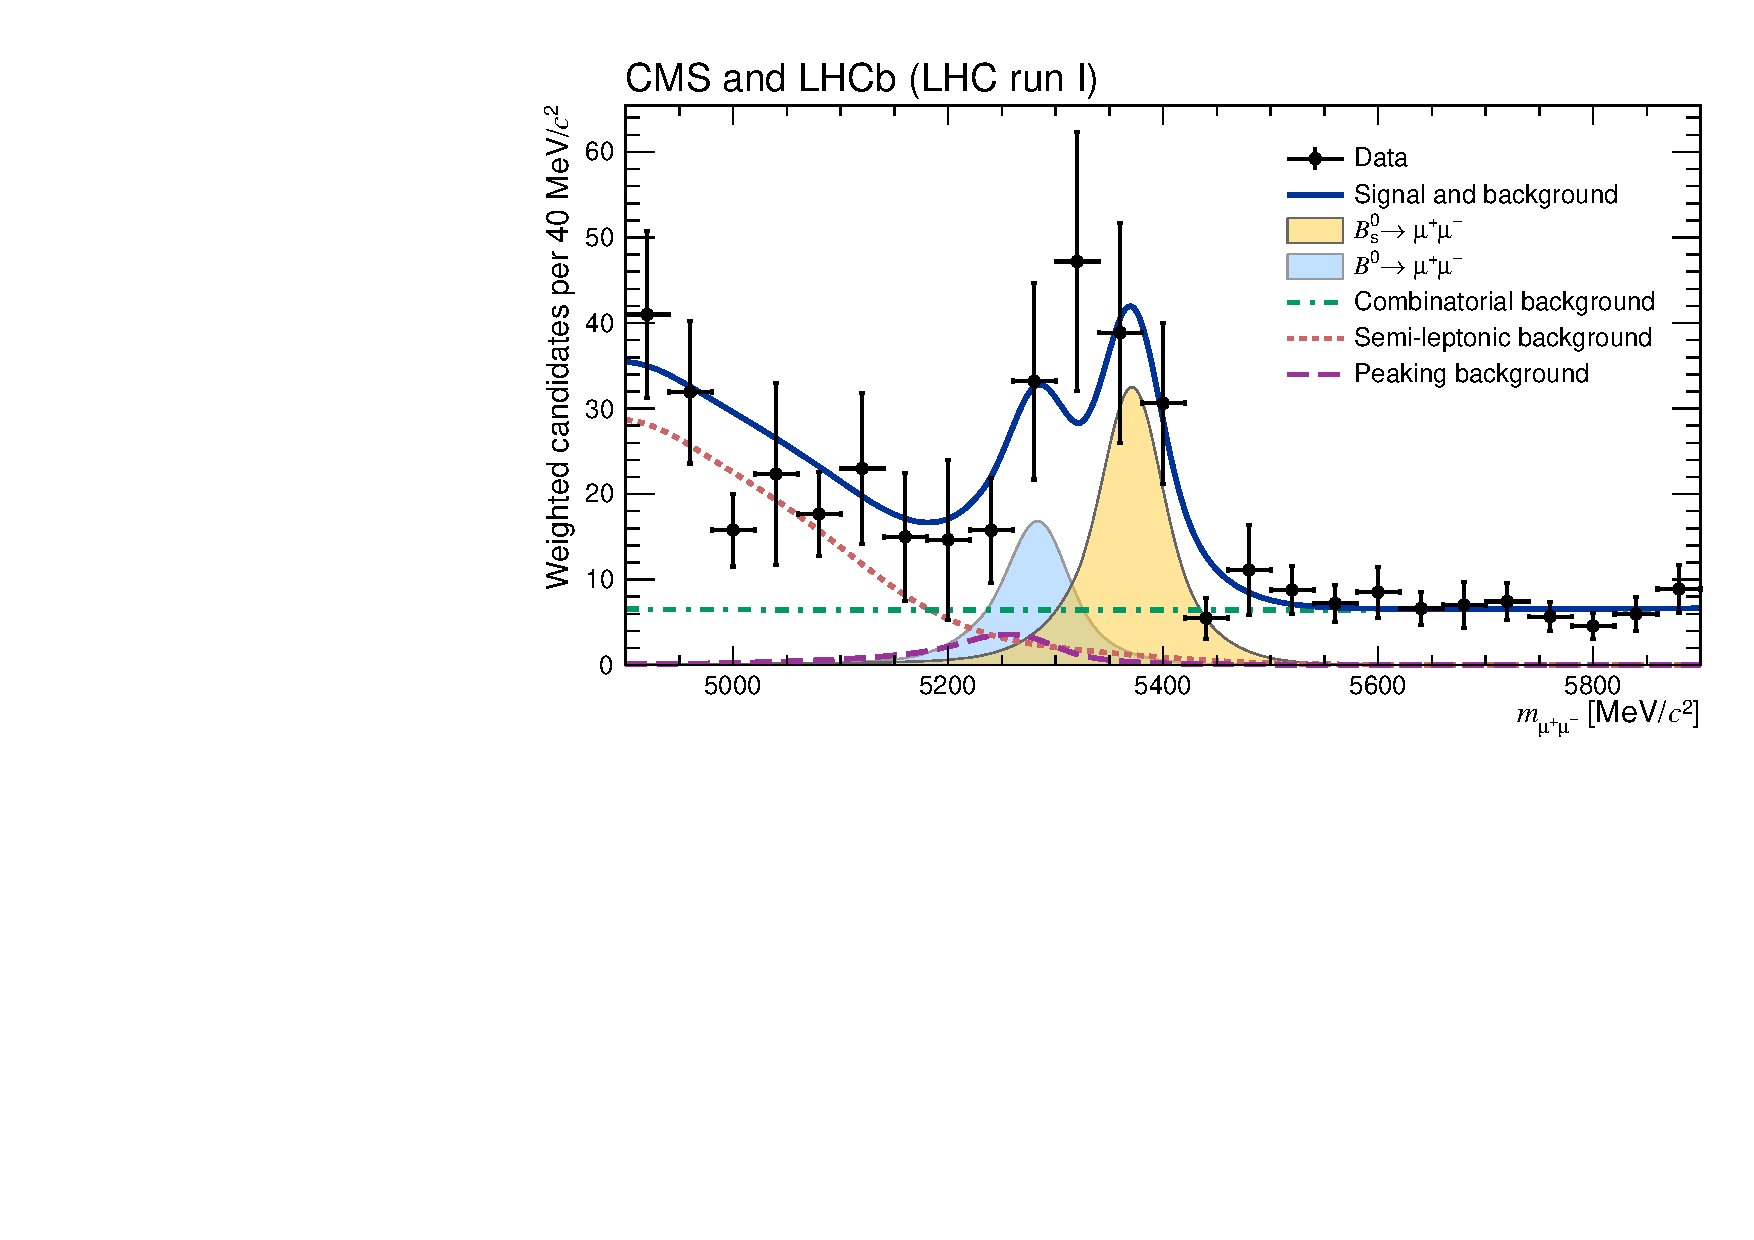
\includegraphics[width= 0.8 \textwidth]{./Figs/Selection/CMSLHCb_fig2.pdf}
        %\caption{ }
       % \label{fig:BDTSsig}
    %\end{subfigure}
   % ~ %add desired spacing between images, e. g. ~, \quad, \qquad, \hfill etc. 
      %(or a blank line to force the subfigure onto a new line)
   % \begin{subfigure}[b]{0.4\textwidth}
      % 
\includegraphics[width=\textwidth]{./Figs/placeholder.jpeg}
      %  \caption{ }
     %   \label{fig:BDTSbkg}
  %  \end{subfigure}
  %  \caption{Weighted dimuon invariant mass spectrum from combined analysis of CMS and LHCb Run~1 data for \bmumu Branching Fraction measurements~\cite{CMS:2014xfa}. Backgrounds included in the mass fit are mis-identified semi-leptonic decays in red, mis-identified \bhh decays in purple and long lived combinatorial background in green. }
   % \label{fig:LHCbCMS}
%\end{figure}

%{\it I could put a plot showing the mass plot from the previous analysis or I could make a plot something like Siim has to illustrate what i mean but that feels a bit like copying!}
%Separating the backgrounds from the \bsmumu decays can be done relatively straightly forwardly for many of the background processes by taking advantage of the obvious differences between the background and \bsmumu decays. However, distinguishing \bsmumu decays from long lived combinatorial backgrounds, and mis-idetificed \bhh and semi-leptonic decays is more challenging and \bsmumu decays must be sacrificed in order to remove a sufficient about of the background processes for the analysis to be performed. For the effective lifetime analysis the \bdmumu decay is not relevant and is therefore a background, however since the decays are extremely similar the \bsd masses are the only way to seperate the decays.

\section{Simulated Particle Decays}
\label{sec:MCsamples}
Simulated particle decays, as described in Section~\ref{SoftwareSimulation}, are used to develop the selection and analysis of \bmumu decays. Large clean samples of simulated decays are needed to separate signal decays from background decays and to understand the impact of selection criteria on decays present in data. 
Many different simulated decay types have been used over time for the development of the selection and analysis of \bmumu decays, however only the simulated decays used for studies documented in this thesis are listed in Table~\ref{tab:MC_decays} along with the data taking conditions and simulation versions used to generated the decays.
\begin{table}[htbp]
\begin{center}
%%\begin{tabular}{p{6cm}p{2.5cm}p{2cm}p{3cm}}                                                                                                           
\begin{tabular}{p{0.45 \textwidth}p{0.15 \textwidth}p{0.15 \textwidth}p{0.15 \textwidth}}
\hline
Decay & Data taking conditions & Simulation version & Generated events \\ \hline 
\multicolumn{4}{c}{{\it Stripping selection studies selection}}  \\ \hline 
\bsmumu& 2012& sim06b  & 2 M \\ 
\bdmumu& 2012& sim06b  & 2 M\\ 
\bdkpi& 2012& sim06b  & 1 M\\ 
\bujpsik& 2012& sim06b  & 1 M\\ \hline 
\multicolumn{4}{c}{{\it Multivariate classifier training}}  \\ \hline
\bbbarmumux, {\footnotesize p~$>$~3~\gevc, 4.7~$< M_{\mu^{+} \mu^{-} <$~6.0~\gevcc, DOCA~$<$~0.4mm, 1~$<$~PtProd~$<$~16~\gevc}
                        & 2012  & sim06b                & 8.0 M      \\
\bbbarmumux, {\footnotesize p~$>$~3~\gevc, 4.7~$< M_{\mu^{+} \mu^{-} <$~6.0~\gevcc, DOCA~$<$~0.4mm,   PtProd~$>$~16~\gevc}
                        & 2012  & sim06b                & 6.6 M\\
\bsmumu                 & 2012  & sim06b                & 2 M \\ \hline
\multicolumn{4}{c}{{\it Analysis method development}}  \\ \hline 
\bsmumu& 2011 & sim08a   & 0.6 M  \\ 
& 2012 & sim08i  & 2 M \\ 
& 2015& sim09a  & 2 M \\ 
& 2016& sim09a  & 2 M ? \\ %Is this correct? I thought in the ntuples we have a lot more 2015 than 2016 MC? 
\bdkpi& 2011& sim08b  & 0.8 M  \\ %11102003
& 2012& sim08g  & 8.6 M \\ 
& 2015& sim09a  & 4 M  \\ 
& 2016& sim09a   & 8.2 M \\ 
\bskk   & 2012& sim08g  & 7.2 M \\ %13102002, 2016 is sim09a 4.1 M per pol, 2011 is sim-8b and 0.8 M per pol
& 2015& sim09a   & 4 M \\  \hline
\end{tabular}
\vspace{0.7cm}
\caption{Simulated decays used for developing the selection and the analysis of \bsmumu listed according to the studies the decays are used in. Cuts are applied to \bbbarmumux decays as they decays are generated, these cuts are included alongside the decay type and are applied to the muon momenta, invariant mass of the muons, the distance of closest approach of the muons and the product of the transverse momenta of the muons.}
\label{tab:MC_decays}
\end{center}
\vspace{-1.0cm}
\end{table}

There exist multiple versions of the simulation because it is updated as understanding of the detector increases and to incorporate differences in data taking conditions, such as the trigger lines or center-of-mass energy, used each year of data is collected. Similar simulation versions must be used to compare different types of simulated decays or data taking conditions so that differences are not masked by variations in the simulation of the decays. The simulated decays in Table~\ref{tab:MC_decays} listed under the studies they are used in. 

Simulated \bbbarmumux decays are used to understand the combinatorial background of \bmumu decays, however producing a large enough sample of these decays to be useful is computational expensive and produces large output files to save generated decays. Therefore cuts are applied at the generation level for \bbbarmumux decays to reduce the size of the samples that are saved and to speed production. The cuts, listed in Table~\ref{tab:MC_decays}, are applied on the muon momenta, the reconstructed mass of the muon pair, the product of the momenta of the muons and the distance of closest approach of the two muon. %The generator level cuts save a factor of 5 of what needs to be saved, striping filtering also reduces it by a factor of 10! The information is in the LHCb-ANA-2013-032, the 2012 bbbarmumux sample corresponds to 7fb-1.
  
%The development of the selection and analysis of \bsmumu decays requires the use of simuluated decays, as described in Section X. The reconstucted \bsmumu candidates come for a range of different different processes, as already discussed, in order to seperate real \bsmumu decays from the background, large clean samples of simulated decays are used so that the differences between signal and background decays can be understood. Futhermore simulated samples are needed to understand 

 


%Simulated \bsmumu, \bdmumu, \bdkpi and \bujpsik decays for 2012 data taking condition are used for studying the stripping selection in Section X.

%The training and testing of multivarite classifiers in Section X uses simulated \bsmumu and \bbbarmumux decays for for 2012 data taking conditions.
 
%Simulated events for \bsmumu, \bskk and \bdkpi for data taken in 2011, 2012, 2015 and 2016 are used for developing the analysis method in Chapter X. 

%The production of simulated events is constantly being developed as understanding of the detector increases and to include changes made for each data is recorded at theLHC. Therefore there exists a number of different simulation versions that can be used to simulate events.

%Each year data is collected at LHCb the conditions the experiment operates at and the proton collisions delivered by the LHC change. These changes include differences in the the selection used in the trigger for each year and increases in the centre of mass energy of proton collisions. 

%Therefore to understand data collected in different years simulated events from each year of data taking is needed, it is important to use similar simulation versions for each year so that the difference in the data taking conditions are not masked by differences in simulation versions. Simiarly for training multivarite classifiers consistent simulation versions are needed for the signal and background samples so that difference between signal and background distributions are not masked by differences in simulation versions.

%In general the stripping selections are applied to simulated events, however events that do not pass the stripping selection are still saved and can be used after reprocessing the simulated events. However simulation conditions can be set up so that events that do not pass the stripping selection are discarded and can never be used and also cuts can be applied on particles when they are generated before the detector response is simulated and the events are reconstructed. This is used when a very large same of simulated events needs to be generated in order to have a suitably large same of events reconstructed and is the case for the samples of \bbbarmumux simulated events.

%Two simulated samples of \bbbarmumux is used to understand the long lived combinatorial background and for the training of the multivariate classifier in Section \ref{sec:BDT}. For these samples events that did not pass the stripping selection have not been saved and requirements were applied to the generated events. 
%Simulated \bsmumu events with the same simulation version are also used for training the multivariate classifier to keep the simulation condition consistent.
On the whole simulated decays accurately model what occurs in data, however there are a couple of area where the simulation falls short of reality.
%Although in general simulated events accurately model what occurs in data there are several areas where this is not the case. 
The distributions of particle identification variables and properties of the underlying proton-proton collision, such as the number of tracks in an event, are not well modelled in the simulation. %Have I said what an event is?
The mis-modelling of particle identification variables can be corrected for using the PIDCalib package~\cite{} and simulated decays can be re-weighted using information from data to accurately model the under lying event, this re-weighting is described in Section~\ref{sec:signalDTpdf}. 


\section{Candidate selection for branching fraction measurements}
\label{sec:BFsel}
The selection of \bmumu decays occurs in several steps, the first step is choosing what requirements to place on the trigger (Sect.~\ref{sec:BFtrigger}) which is followed by a cut based selection to remove obvious background events (Sect.~\ref{sec:cutbasedsel}. Then particle identification variables (Sect.~\ref{sec:BFpid}) to reduced background events from mis-identified semi-leptonic and \bhh decays and finally multivariate classifiers (Sect.~\ref{sec:MVC}) are used as the last step in the selection to reduced the backgrounds to a low enough level so that the \bmumu \BFs can be measured.% from the data.

The measurement of the \bdmumu and \bsmumu \BFs are described in Chapter~\ref{sec:BFanalysis} and requires \bujpsik and \bhh decays to determine the branching fractions from the observed number of \bmumu decays in data. Furthermore \bsjpsiphi decays used to verify steps of measurement process. The selection criteria for these decays are kept as similar as possible to the selection of \bmumu decays and will be described alongside the signal selection.


\subsection{Trigger}
\label{sec:BFtrigger}

%The trigger is the first step in the selection process and the structure of the trigger is described in Section X. Since \bsmumu decays are very rare a broad set of trigger requirements is used in order to keep a high proportion of \bsmumu decay at this step of the selection. Specific trigger lines are not used in the selection but rather the combined results of a large selection of trigger lines at each level of the trigger. The combinations of trigger lines used are the L0Global, Hlt1Phys and Hlt2Phys triggers. The L0Global trigger combines all trigger lines present in the L0 trigger, it selects an event provided at least one L0 selects it and rejects an event if no L0 trigger selects it. The Hlt1Phys and Hlt2Phys triggers are very similar to the L0Global trigger except that decisions are based only trigger lines related to physics processes and HLT trigger lines used for calibration are excluded. 

%Different trigger decisions on these lines are used to select decays for the Branching Fraction and effective lifetime analyses. The Branching fraction selection imposed the loosest trigger requirements by requiring a event to pass the `Dec' decision at each trigger level as illustrated in set `A' of Table X. Trigger decisions are defined in Section X. The effective lifetime analysis has slightly more constrained trigger requirement, requiring an event passes either the `TIS' or `TOS' decision at each level of the trigger as illustrated in set `B' of Table X. The trigger choice for the effective lifetime is motivated by the determination of the acceptance function in Section X. 
%The selection criteria used in trigger lines and the specific lines included in the trigger change with each year of data taking, the dominant lines for triggering \bsmumu decays for each year are shown in Table~X. 

%Events are required to be either TIS, triggered independent of signal or TOS, triggered on signal, on the trigger lines used at each level of the trigger.
%The selection criteria used in trigger lines and the specific lines included in the trigger change with each year of data taking, the dominant lines for triggering \bsmumu decays for each year are shown in Table~X. 
%Slightly different trigger requirements are used to select \bhh decays used to develop and validate the effective lifetime analysis, the same broad trigger lines are used but the requirement on the output varies depending on the use of the \bhh events. The are two sets of trigger requirements, set `A' and `C', in Table~\ref{tab:triggers} are used to select \bhh decays, it will be made clear in later sections where \bhh decays are used which trigger requirements are imposed. 

The trigger, described in Sect.~\ref{Trigger}, is the first step in the selection, it selects events that could contain an interesting particle decays and these events are saved to be used in physics analyses. Candidates from different particle decays are reconstructed from events that have passed the trigger. For each candidate it is useful to know whether is was a component in that candidate that caused the event to be selected by a trigger line or if it was another part of the event. There are several different decisions that identify this;
\begin{itemize}
\item TOS, triggered on signal - a candidate is identified as TOS if only information from the candidate was enough to cause a trigger line to select the event
\item TIS, triggered independent of signal - a candidate is identified as TIS if part of the event independent of the candidate was enough to cause a trigger line to select the event
\item DEC - a candidate is identified as DEC if anything in the event caused a trigger line to select an event. This includes TIS and TOS decisions and also when a combination of information from the candidate and something else in the event caused a trigger line to select the event
\end{itemize}

\bsmumu decays are very rare decays and therefore trigger requirements used to select these decays are chosen to keep a high efficiency is kept at this step of the selection. The trigger lines L0Global, Hlt1Phys and Hlt2Phys are used and candidates are required to identified as DEC at each level of the trigger. These trigger lines combine the decisions of many individual lines used in the trigger which allows a high efficiency to be achieved for selecting \bsmumu decays. The L0Global trigger combines all trigger lines present in the L0 trigger, it selects an event provided at least one L0 trigger line selects it and rejects an event if no L0 trigger selects it. The Hlt1Phys and Hlt2Phys triggers are very similar to the L0Global trigger except that decisions are based only trigger lines related to physics processes and HLT trigger lines used for calibration are exclude.

The same trigger requirements to identify \bmumu decays are used to select \bujpsik and \bsjpisphi decays and slightly different trigger requirements are used for \bhh decays. \bhh decays are required to be triggered independant of signal by the L0Global and Hlt1Phys trigger lines and triggered on signal by at the HLT2 level by specific trigger lines designed to select \bhh decays. The TIS desicion is used for \bhh decays to reduce the difference between the dominant lines that trigge \bhh and \bmumu decays, however the efficiency of TIS decisions is quite low at the HLT2 level therefore TOS decisions are used there to high a high enough number of decays.

%Slightly different trigger decisions are used to select \bhh, \bujpsik and \bsjpisphi decays ...... (Prehaps indicate that this will be made clear later? Or just say what is used for the normalisation?) B2H is TIS at L0 and HLT1 and TOS for a specifice HLT2 line B2HH. I think the other decays are the same as Bs2MuMu.
 %but the same trigger lines are used. To be useful as a validation channel the efficiency of the trigger requirements as a function of the decay time needs to be similar to the \bsmumu triggers, this is achieved by requiring \bhh decays to be TIS at each level of the trigger. %\bhh candidates are required to be TIS at each level of the trigger, this trigger decision is used to ensure the trigger efficiency to select \bhh decays is similar to the \bsmumu trigger efficiency. 

The requirements imposed on the trigger to select \bsmumu, \bhh, \bujpsik and \bsjpisphi decays is shown in Table~\ref{tab:triggers}.

\begin{table}[htbp]
\begin{center}
\begin{tabular}{ll}
\hline
Trigger Line& Trigger decision \\ \hline
%\multicolumn{2}{c}{{\it set A}} \\ \hline
%L0Global& Dec\\
%Hlt1Phys& Dec \\
%Hlt2Phys& Dec \\ \hline
\multicolumn{2}{c}{{\it Select \bsmumu, \bujpsik, \bsjpsiphi decays}} \\ \hline
L0Global& DEC \\
Hlt1Phys& DEC \\
Hlt2Phys& DEC \\ \hline
\multicolumn{2}{c}{{\it Select \bhh decays}} \\ \hline
L0Global& TIS\\
Hlt1Phys& TIS \\
Hlt2B2HHDecision& TOS \\ \hline
\end{tabular}
\vspace{0.7cm}
\caption{Trigger lines used to select \bsmumu, \bhh, \bujpsik and \bsjpisphi decays.}% Set `A' is used to select decays for the Branching Fraction analysis. Set `B' is used to select \bsmumu decays for the effective lifetime analysis. Sets `A' and `C' are used to select \bhh decays used to develop the \bsmumu effective lifetime analysis.}
\label{tab:triggers}
\end{center}
\vspace{-1.0cm}
\end{table}


%There was a problem with the implementation of the Hlt2Phys Dec decision in 2016 simulated events.%, the decision returned was always 1.  
%This only affect the selection of \bhh decays. In order to emulate this trigger a combination of Hlt2 lines that select \bhh events, listed in Table~\ref{tab:HltDecEmulation}, is used instead of HLT2Phys when the Dec decision is required. 

%\begin{table}[ht]
%\begin{center}
%\begin{tabular}{l}
%\hline
%\bhh trigger lines \\ \hline
%Hlt2Topo2BodyDecision Dec  \\
%Hlt2B2HH Lb2PPiDecision Dec \\
%Hlt2B2HH Lb2PKDecision Dec \\
%Hlt2B2HH B2PiPiDecision Dec \\
%Hlt2B2HH B2PiKDecision Dec \\
%Hlt2B2HH B2KKDecision Dec  \\
%Hlt2B2HH B2HHDecision Dec \\ \hline

%\end{tabular}
%\vspace{0.7cm}
%\caption{Trigger lines used to emulate the Hlt2Phys$\_$Dec decision for \bhh data and simulated events.}
%\label{tab:HltDecEmulation}
%\end{center}
%\end{table}

\subsection{Cut based selection}
\label{sec:cutbasedsel}
%http://lhcb-release-area.web.cern.ch/LHCb-release-area/DOC/stripping/config/stripping20/dimuon/strippingbs2mumulineswidemassline.html 
The \bmumu candidates that passed the required trigger decisions are refined by a cut based selection. These selection cuts are aimed at removing obvious backgrounds by exploiting the differences between real \bmumu decays and the backgrounds that mimic them. The selection of \bhh, \bujpsik and \bsjpisphi decays is kept as close as possible to that of \bmumu decays. The cut based selection is composed of two parts; the stripping selection and the offline selection. 

The stripping selection, as described in Section~\ref{Software_Simulation}, is applied to all events that pass the trigger. It consists of individual stripping lines that select reconstructed candidates for specific decays, the development of the stripping selection is described in Sections~\ref{strippingold}~and~\ref{strippingstudies}.% of stripping lines  by exploiting differences between the decays and the backgrounds that mimic them. 



%The selection of \bsmumu and \bhh decays for the \bsmumu effective lifetime measurement uses the same stripping lines as those in the \bmumu Branching Fraction measurements. These lines were designed at the start of Run~1 by studying the efficiencies of different selection cuts from simulated events \cite{}. However since then improvements have been made to the simulation of particle decays at LHCb, therefore it is prudent to check the accuracy of the selection efficiencies with updated simulated events and investigate where improvements can be made to the efficiency of the stripping selection used to select \bsmumu events. These studies are detailed in Sections~\ref{strippingold} and~\ref{strippingstudies}.

The offline selection cuts are applied to the output of the stripping selection. Overall stripping selection imposes loose selection requirements onto \bmumu candidates so that as much information as possible is still available to develop the analysis and understand background events after the stripping selection. Therefore the offline selection further refines the data, removing background candidates. The full set of cuts applied in the stripping and offline selection to select \bmumu and other relevant decays from Run~1 and Run~2 data are presented in Section~\ref{finalloosesel}. 


 
%REDO THIS AFTER WORKING OUT EXACTLY WHAT DETAILS I THINK ARE IMPORTANT TO INCLUDE!
%The stripping selection is a set of loose cuts that are applied to reconstructed events that have passed the trigger. The stripping selection consist of `lines' that are taylored to select particular decays. The aim of stripping lines is to reduce the size of the data sets collected by the experiment to a managable size on which tighter selection cuts to be developed and applied offline. Events that do not pass the selection cuts in the stripping lines are not directly avaliable to physics analyses. Therefore the cuts applied in the stripping lines are designed to remove obvious background events whilst keeping a high efficecny on the decay of interest. Restraints are placed on the amount of data that can pass the stripping selection for a particular analysis, typically this is set to be 0.05$\%$ of the original LHCb data set size for events that are saved in DST files. 
%This paragraph is ok.



\subsubsection{Development of the stripping selection}
\label{strippingold}

%The stripping selection used to select \bsmumu and \bhh decays for the \bsmumu effective lifetime measurement uses the same stripping lines as the selection of \bmumu decays for the Branching Fraction measurement. 
The stripping selections to selectio all decays necessary for the measurement of the \bmumu branching fractions were designed at the start of Run~1 by studying the efficiencies of different selection cuts from simulated events~\cite{Diego}. However since then improvements have been made to the simulation of particle decays at LHCb, therefore it is prudent to check the accuracy of the selection efficiencies with updated simulated events and investigate where improvements can be made to the efficiency of the stripping selection used to select \bmumu events.


%In addition to \bmumu and \bhh decays the measurement of the \bmumu Branching Fractions requires \bujpsik decays. \bdkpi and \bujpsik decays are used to normalise the number of observed \bsmumu decays to the number created in $pp$ collisions. 

There are four seperate stripping lines that select \bmumu, \bujpsik, \bsjpisphi and \bhh candidates, the selection of the all decays is kept as similar as possible to the signal selection to avoid introducing systematic uncertainties in the normalisation procedure of the branching fraction described in Chapeter~\ref{sec:BFanalysis}. However, the selection of \bujpsik and \bsjpsiphi decays must diverge from the \bmumu selected due to additional particles in the final state of the decay. Any changes made to the \bmumu stripping selection to improve the selection efficiency must be included in the selection of the other decays to keep the systematic uncertainties under control, this is particularly important for \bhh and \bujpsik decays. %, therefore all three stripping lines must be studied together. 
The stripping selection cuts applied for the Run~1 Branching Fraction analysis~\cite{CMS:2014xfa, Aaij:2013aka} to select \bmumu, \bujpsik, \bsjpisphi and \bhh candidates are listed in Table~\ref{tab:PreviousStripping1} and~\ref{tab:PreviousStripping2} .


%The stripping selection cuts and cuts applied during the reconstruction of particle decays for the Run 1 \bmumu Branching Fraction analysis \cite{} to select \bmumu, \bhh and \bujpsik are shown in Table X. The selection of \bujpsik and \bhh decays is kept as similar as possible to the selection of \bsmumu decays to avoid introducing systematic errors when \bhh and \bujpsik decays are used in the normalisation for the Branching Fraction measurement. The selection of \bujpsik event must diverge from the \bsmumu selection due to additoinal particles in the final state of the decay. The stripping selection imposes more cuts to select \bhh decays compared to \bsmumu because \bhh decays are much more abundant therefore extra cuts are needed to reduce the number of events passing the stripping to an acceptable level. The cuts applied to \bhh in the stripping are the later applied to \bsmumu events after the stripping selection. 
%The measurement of the \bsmumu Branching Fraction, described in Chapter X, uses \bujpsik and \bdkpi decays to normalise the number of observed \bsmumu decays to the number created in proton-proton collisions. There are three stripping lines that select \bmumu, \bujpsik and \bhh candidates, where $h = K, \pi$, the selection of the normalisation channels is kept as similar as possible to the signal selection to avoid introducing systematic uncertainties in the normalisation procedure. However, the selection of \bujpsik decays must diverge from \bsmumu due to additional particles in the final state of the decay. Any changes made to the \bmumu stripping selection to improve the selection efficiency must be included in the selection to the normalisation channels to keep the systematic uncertainties under control, therefore all three stripping lines must be studied together. The stripping selection cuts applied for the Run~1 Branching Fraction analysis~\cite{} to select \bmumu, \bhh and \bujpsik decays are listed in Table~\ref{tab:PreviousStripping}.

%\afterpage{
%\begin{landscape}
%\vspace*{\fill}
\begin{table}[htbp]
\begin{center}
\begin{tabular}{l|ll}
\hline
  Particle              & \bsmumu                                     & \bhh                                  \\
\hline             
\bsd         & |M - M$_{PDG}$| $<$ 1200 \mevcc              & |M - M$_{PDG}$| $<$ 500 \mevcc     \\          
                      & DIRA > 0                                    & DIRA > 0                             \\       
                      & FD $\chi^{2}$ $>$225                        & FD $\chi^{2}$ $>$225              \\ 
                      & IP $\chi^{2}$ $<$ 25                         & IP $\chi^{2}$ $<$ 25                \\            
                      & Vertex $\chi^{2}$/ndof < 9                   & Vertex $\chi^{2}$/ndof < 9                \\   
                      & DOCA $<$ 0.3 mm                             & DOCA $<$ 0.3 mm                            \\               
                      &                                             & $\tau$ $<$ 13.248 \ps                      \\
                      &                                             & $p_{T}$ $>$ 500 \mevc                      \\
\hline             
Daughter $\mu$ or $h$   & Track $\chi^{2}$/ndof < 3                 & Track $\chi^{2}$/ndof < 3            \\       
                        & isMuon = True                             &                                             \\ 
                        & Minimum IP $\chi^{2}$ $>$ 25               & Minimum IP $\chi^{2}$ $>$ 25             \\                   
                        &    $p_{T}$ $>$ 0.25 \gevc                   & 0.25 \gevc $<$ $p_{T}$ $<$ 40 \gevc  \\
                        &                                           & ghost probability $<$ 0.3        \\

\hline
\end{tabular}
\vspace{0.7cm}
\caption{Selection requirements applied during the stripping selection for Run~1 data used in the \bmumu Branching Fraction analysis~\cite{CMS:2014xfa, Aaij:2013aka} to select \bmumu and \bhh decays. $M_{PDG}$ corresponds to the Particle Data Group~\cite{Olive:2016xmw} mass of each particle.}%The track $\chi^{2}$/ndof and isMuon cut are applied during the reconstruction.}
\label{tab:PreviousStripping1}
\end{center}
\end{table}
%\vspace*{\fill}
%\end{landscape}
%}


%\afterpage{
%\begin{landscape}
%\vspace*{\fill}
\begin{table}[htbp]
\begin{center}
\begin{tabular}{l|l|l|l}
\hline
  Particle            &\bujpsik                             & Particle   &\bsjpsiphi \\
\hline             
$B^{+}$        & |M - M$_{PDG}$| $<$   500 \mevcc           & \bs         & |M - M$_{PDG}$| $<$   500 \mevcc             \\          
                      & Vertex $\chi^{2}$/ndof < 45         &            &  Vertex $\chi^{2}$/ndof < 75             \\       
                      & IP $\chi^{2}$ $<$ 25                &            &  IP $\chi^{2}$ $<$ 25               \\ \hline   
\jpsi                & |M - M$_{PDG}$| $<$   100 \mevcc      & \jpsi      &  |M - M$_{PDG}$| $<$   100 \mevcc     \\
                    & DIRA > 0                             &           &   DIRA > 0           \\
                    & FD $\chi^{2}$ $>$ 225                &           & FD $\chi^{2}$ $>$ 225        \\
                    & Vertex $\chi^{2}$/ndof < 9           &           & Vertex $\chi^{2}$/ndof < 9       \\  
                    &   DOCA $<$ 0.3 mm                   &            & DOCA $<$ 0.3 mm      \\  
\hline             
$\mu^{\pm}$               & Track $\chi^{2}$/ndof < 3           &$\mu$       &  Track $\chi^{2}$/ndof < 3 \\       
                    & isMuon = True                      &            &isMuon = True    \\ 
                    & Minimum IP $\chi^{2}$ $>$ 25        &            & Minimum IP $\chi^{2}$ $>$ 25    \\                   
                    &  0.25 \gevc $<$ $p_{T}$            &            &  0.25 \gevc $<$ $p_{T}$    \\
\hline
$K^{+}$             & Track $\chi^{2}$/ndof < 3           & $\phi$           &  |M - M$_{PDG}$| $<$   20 \mevcc  \\
                    & $p_{T}$ $>$ 0.25 \gevc              &           &  Minimum IP $\chi^{2}$ $>$ 4  \\
                   & Minimum IP $\chi^{2}$ $>$ 25         & K$^{\pm}$           & Track $\chi^{2}$/ndof < 3  \\
                 &                                   &                       & $p_{T}$ $>$ 0.25 \gevc     \\
\hline
\end{tabular}
\vspace{0.7cm}
\caption{Selection requirements applied during the stripping selection for Run~1 data used in the \bmumu Branching Fraction analysis~\cite{CMS:2014xfa, Aaij:2013aka} to select \bujpsik and \sjpsiphi decays. $M_{PDG}$ corresponds to the Particle Data Group~\cite{Olive:2016xmw} mass of each particle.}%The track $\chi^{2}$/ndof and isMuon cut are applied during the reconstruction.}
\label{tab:PreviousStripping}
\end{center}
\end{table}
%\vspace*{\fill}
%\end{landscape}
%}


The variables used in the stripping selection are:
\begin{itemize}
\item the reconstructed mass, $M$ - the mass and momenta of the decay products of the $B$ meson (or \jpsi) are combined to provide its reconstructed mass. Cuts on the mass remove candidates with a reconstructed mass far from the expected mass that are clearly backgrounds. Loose mass requirements are made on for the \bmumu selection to allow for the study of semi-leptonic backgrounds that have a mass less than the \bsd mass when mis-identified as \bmumu decays;
\item the ``direction cosine'', DIRA - this is the cosine of the angle between the momentum vector of the particle and the vector connecting the production and decay vertices\footnote{The production vertex of the $B$ or the primary vertex is identified by extrapolating the $B$ meson momentum vector towards the beam axis. The closest vertex to the intersection of the $B$ momentum and the beam axis is assigned as the primary vertex.} of the particle. For correctly reconstructed candidates the direction cosine should be very close to one, requiring candidates to have positive value ensuring events are travelling in the incorrect direction are removed;
\item the flight distance (FD) \chisqd $ $- this is computed by performing the fit for the production vertex of a particle but including the tracks from its decay products that originate from the decay vertex in the fit as well. For a $B$ meson the FD \chisqd is likely to be large because $B$ mesons have long lifetimes therefore the tracks of its decays products will not point towards the production vertex;
\item track fit \chisqd/$ndof$ - provides a measure of the quality of a fitted track, placing an upper limit removes poor quality tracks and backgrounds composed of poorly reconstructed decays;
\item vertex fit \chisqd/$ndof$ - provides a measure of how well tracks can be combined to form a vertex, placing an upper limit removes poorly constrained vertices and backgrounds composed of poorly reconstructed decays;
\item distance of closest approach (DOCA) - this is the distance of closest approach of two particles computed from the straight tracks in the VELO. For the decay products of a particle, for example the muons from \bmumu, this distance would ideally be zero because the muons originate from the same vertex;
\item decay time, $\tau$ - is the length of time a particle lives as it travels from its production vertex to its decay vertex. Applying an upper decay time cut removes unphysical background decays;
\item isMuon - particle identification variable defined in Section~\ref{PID} that returns True for muons and False for other particles;
\item transverse momentum, $p_{T}$ - the component of a particle's momentum perpendicular to the beam axis. Decay products of $B$ mesons are expected to have relatively high \pt due to the heavy $B$ meson masses however an upper limit removes unphysical backgrounds;
\item momentum, $p$ - an upper limit on the momentum of a particle  removes unphysical backgrounds;
\item ghost probability - defined in Section~\ref{Trackrecon} provides the probability of a tracking being composed on random hits in the detector, tracks from the passage of real particles will have a low ghost probability; 
\item impact parameter (IP) \chisqd $ $- this is the change in the fit for a primary vertex (PV) caused by removing one track in the fit. In a \bsmumu decay, the \bsd is produced at the PV therefore it should have a small IP \chisqd value whereas the muons will be displaced from the PV because of the relatively long lifetime of the \bsd and therefore will have a large IP \chisqd;
\item minimum impact parameter (IP) \chisqd $ $- this is the IP \chisqd of the muons with respect to all PVs in the event, this parameter is used to remove prompt muons created at any PV in the event and therefore reduce the prompt combinatorial background. 
\end{itemize}

The stripping selection imposes a greater number cuts to select \bhh decays compared to \bsmumu because \bhh decays are much more abundant therefore extra cuts are needed to reduce the number of events passing the stripping to an acceptable level. The cuts applied to only \bhh decays in the stripping are the later applied to \bsmumu candidates in the offline selection. %The cuts on muon transverse momentum, track \chisqd and isMuon (when used) are applied in the reconstruction and cannot be changed.


\subsubsection{Optimisation of \bsmumu stripping selection}
\label{strippingstudies}


The efficiency of the cuts used in the stripping lines to selecting \bmumu, \bhh and \bujpsik decays are shown in Table \ref{tab:Run1strippingEff}, only cuts that are in common with the \bmumu stripping lines are listed. The efficiencies of \bhh and \bujpsik are studied as well as \bmumu because the selection of these channels must be kept similar to reduce systematic uncertainties in the noramalisation proceedure described in~\ref{}. The efficiencies are evaluated using 2012 sim06 simulated events that have the minimum track \pt, track \chisqd and isMuon requirements imposed. These cuts are applied during the reconstruction and particles that do not pass these requirements are not included in the samples of simulated decays. No trigger requirements have been applied so that only the effect of the stripping selection on the efficiencies can be assessed. During the simulation of particle decays the trigger is run in {\it pass through} mode so that all reconstructed are saved not just those that have passed a trigger line. 


\afterpage{
\begin{landscape}
\vspace*{\fill}
%\begin{sideways}
\begin{table}[htbp]
\begin{center}
\begin{tabular}{p{6cm}cccc}
                  & \multicolumn{3}{c}{Efficiency}  \\ 
\cline{2-5}
Requirement                                  & \bsmumu                   & \bdmumu                       & \bhh                &\bujpsik  \\
\hline
$B$ |M - M$_{PDG}$|                           & (100.00 $\pm$ 0.00)$\%$  & (100.00 $\pm$ 0.00 )$\%$      & (98.25 $\pm$ 0.02)$\%$        & (99.73 $\pm$ 0.02)$\%$ \\
\bsd or \jpsi DIRA                            & (99.41 $\pm$ 0.01) $\%$  & (99.47 $\pm$ 0.01)$\%$        & (99.47 $\pm$ 0.01)$\%$        & (95.83 $\pm$ 0.08)$\%$ \\
\bsd or \jpsi FD $\chi^{2}$                   & (83.74 $\pm$ 0.06) $\%$  & (83.96 $\pm$ 0.06)$\%$        & (83.83 $\pm$ 0.06)$\%$        & (82.90 $\pm$ 0.15)$\%$ \\
\bsd or \jpsi IP $\chi^{2}$                   & (96.78 $\pm$ 0.03) $\%$  & (96.93 $\pm$ 0.03)$\%$        & (97.44 $\pm$ 0.03)$\%$        & (97.52 $\pm$ 0.06)$\%$ \\
\bsd or \jpsi vertex $\chi^{2}$/ndof          & (97.21 $\pm$ 0.03) $\%$  & (97.18 $\pm$ 0.03)$\%$        & (97.68 $\pm$ 0.02)$\%$        & (96.78 $\pm$ 0.07)$\%$ \\
\bsd or \jpsi DOCA                           & (99.82 $\pm$ 0.01) $\%$   & (99.80 $\pm$ 0.01)$\%$        & (99.83 $\pm$ 0.01)$\%$        & (99.58 $\pm$ 0.03)$\%$ \\               

$\mu$, $h$, $K^{+}$ minimum IP $\chi^{2}$    & (80.16 $\pm$ 0.06) $\%$  & (80.62 $\pm$ 0.06 )$\%$        & (79.66 $\pm$ 0.07)$\%$        & (86.98 $\pm$ 0.14)$\%$ \\
\hline
Total after above cuts                  & (71.29 $\pm$  0.07) $\%$  & (71.82 $\pm$ 0.07)$\%$        & (70.97 $\pm$ 0.07)$\%$        & (71.30 $\pm$ 0.18)$\%$ \\
\hline
Total after all cuts      & -                         & -                             & (70.70 $\pm$ 0.07)$\%$        & (62.25 $\pm$ 0.20)$\%$ \\
\hline
\end{tabular}
\vspace{0.7cm}
\caption{Stripping line cut efficiencies for \bsmumu, \bhh and \bujpsik  2012 simulated decays. Selection cuts applied are listed in Table~\ref{tab:PreviousStripping}. Efficiencies have been calculated only for cuts that are present in the \bsmumu stripping, each cut separately and the total efficiencies are given for the listed cuts and the complete set of cuts present in each stripping line. }
\label{tab:Run1strippingEff}
\end{center}
\end{table}
\vspace*{\fill}
\end{landscape}
%\end{sideways}
}


The selection efficiencies are very similar for each stripping cut across the different decays which fits the requirement that the selection of signal and normalisation decays used in the branching fraction measurement are as similar as possible. The similarity of the selection efficiencies for the signal and normalisation decays is further illustrated in Figures~\ref{fig:ratioplotsJpsik} and \ref{fig:ratio_plotsBd2KPi} which show the ratio of selection efficiencies for \bsmumu decays to \bujpsik and \bdkpi decays for a range of selection cuts. With the exception of the \bsmumu and \bujpsik IP $\chi^{2}$ cuts on the daughter particles, the ratio of efficiencies is well within $3\%$ of~1 for the range of cuts values shown. The ratio of the \bsmumu and \bujpsik efficiencies for the daughter particle IP $\chi^{2}$ markedly deviates from unity, showing that the IP $\chi^{2}$ distribution of the muons and kaon are very different as seen previous in~\cite{Diego}. If the FD \chisqd, \bs or \jpsi IP \chisqd and vertex \chisqd selection cuts are applied to the simulated events before the daughter IP $\chi^{2}$ requirement the ratio of \bmumu and \bujpsik efficiencies is much closer to~1. The stability of the ratios of selection efficiencies across a large range of cuts values shows that changing a cut value in the \bmumu selection will have a similar impact on the efficiencies of the normalisation decays. 


\begin{figure}[htbp]
    \centering
    \begin{subfigure}[b]{0.4\textwidth}
        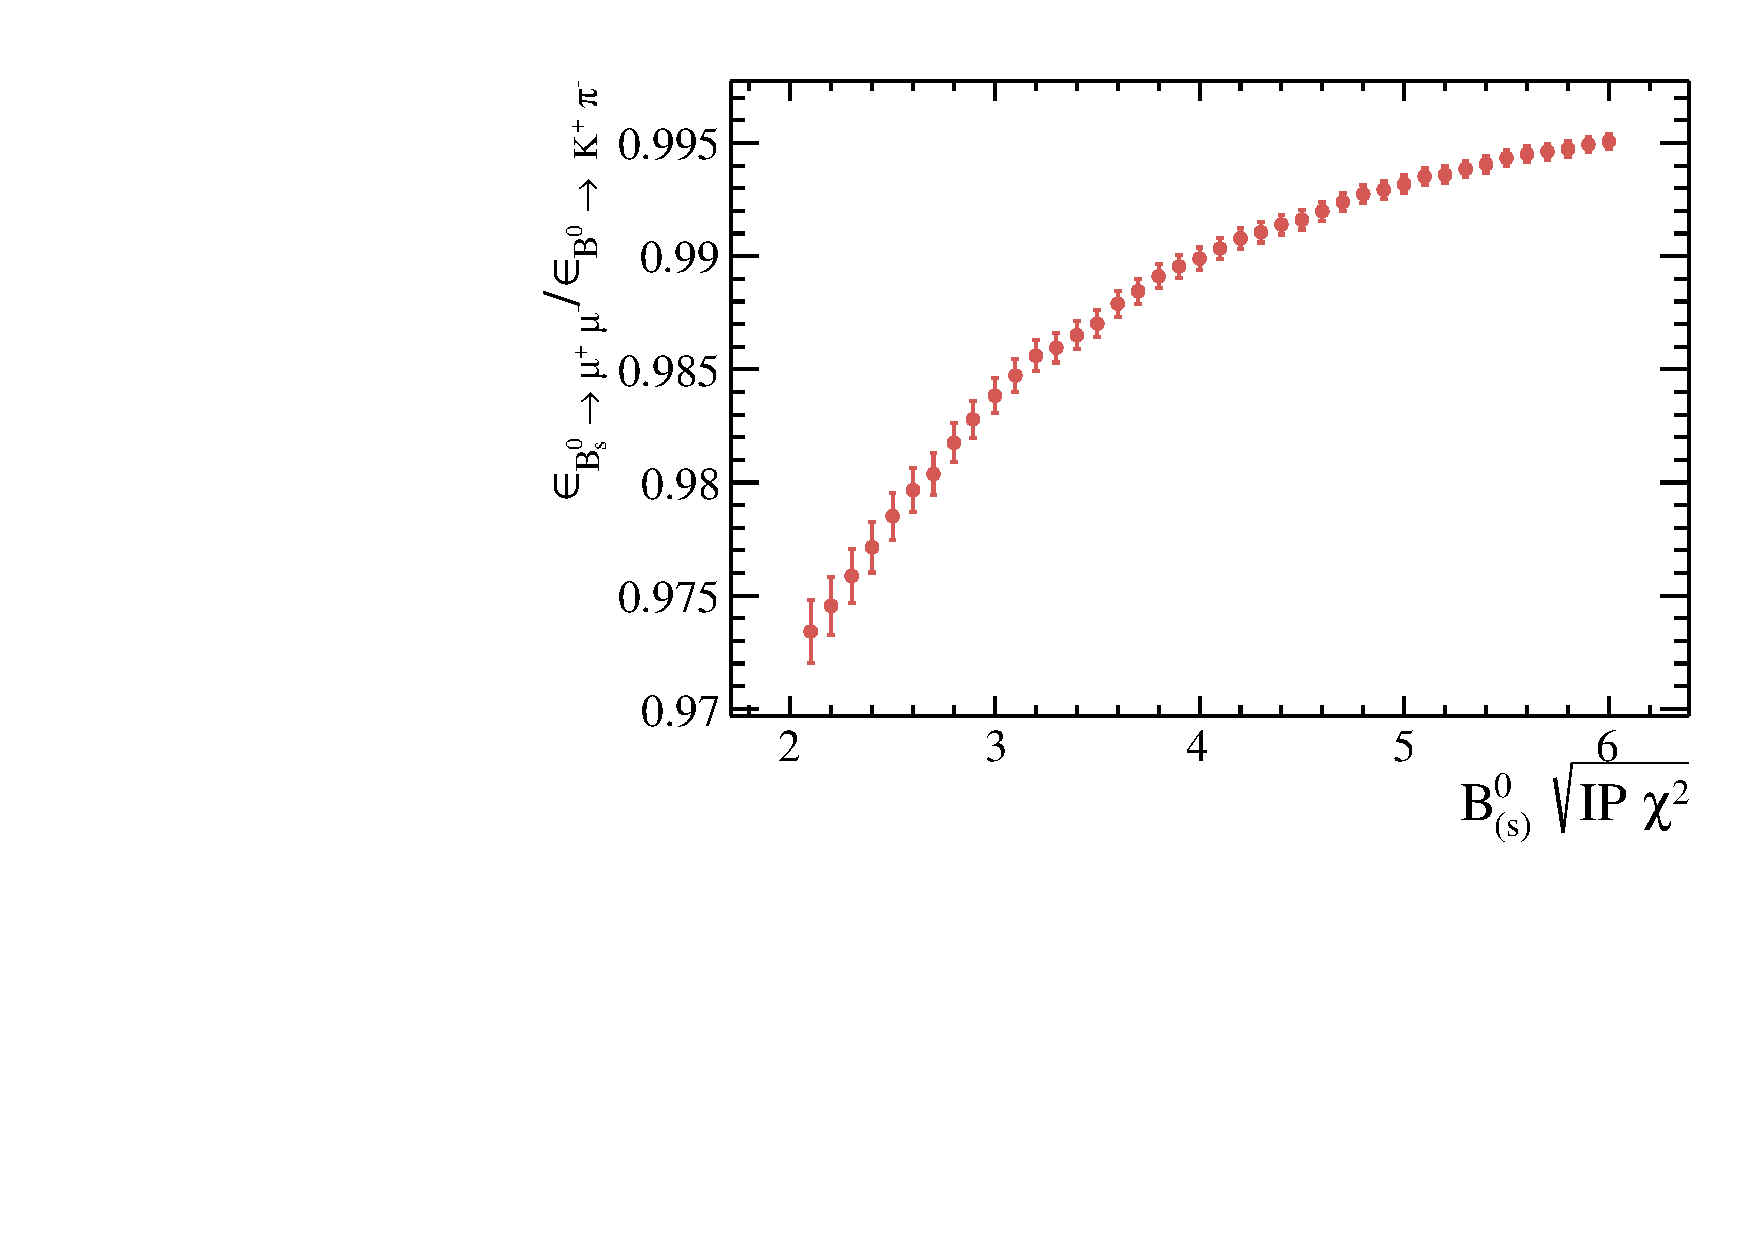
\includegraphics[width=\textwidth]{./Figs/Selection/Bs2MuMu_KPi_IP.pdf}
        %\caption{ }
        %\label{fig:IPS_ratioKPi}
    \end{subfigure}
    ~ %add desired spacing between images, e. g. ~, \quad, \qquad, \hfill etc.                                                                                    
      %(or a blank line to force the subfigure onto a new line)                                                                                                   
    \begin{subfigure}[b]{0.4\textwidth}
        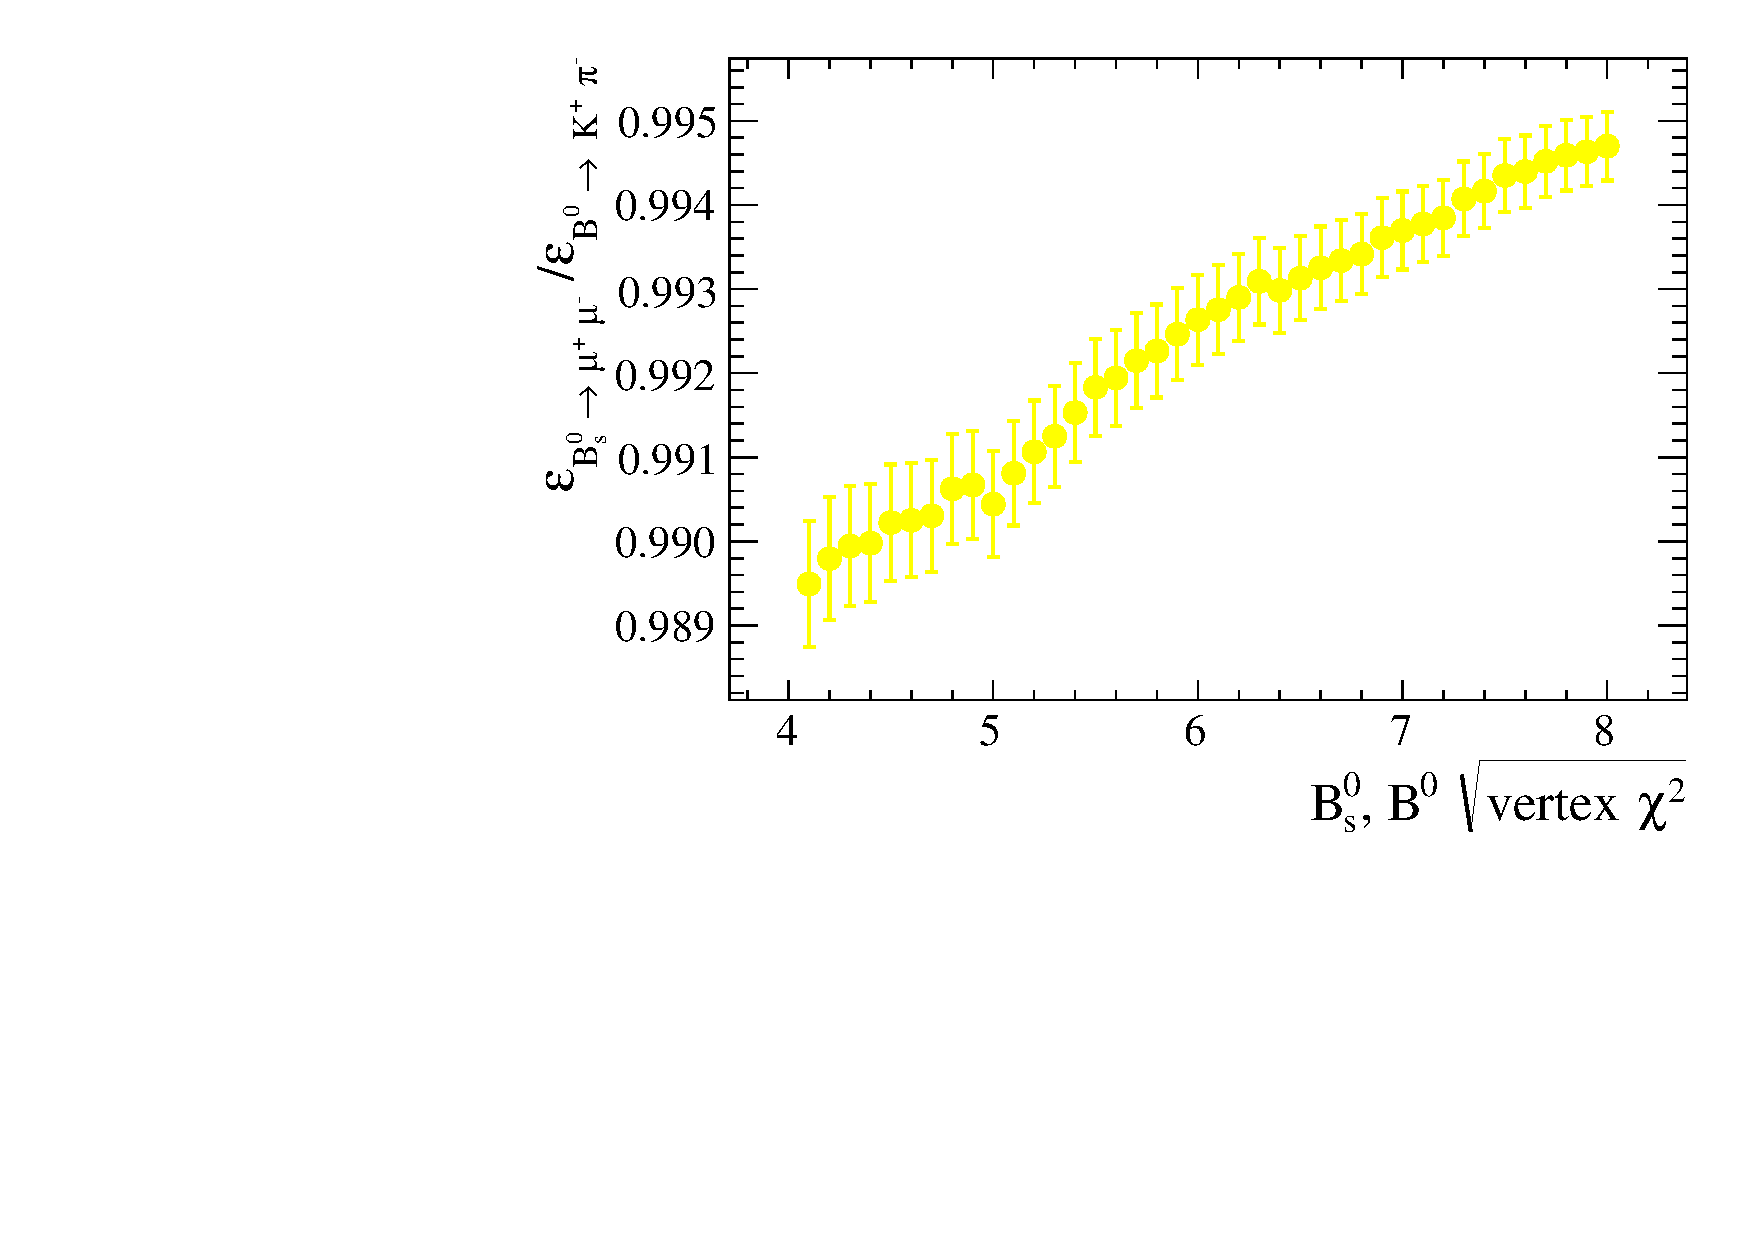
\includegraphics[width=\textwidth]{./Figs/Selection/BSMuMu_KPi_vertex.pdf}
        %\caption{ }
        %\label{fig:CHI2_ratioKPi}
    \end{subfigure}
    ~ %add desired spacing between images, e. g. ~, \quad, \qquad, \hfill etc.                                                                                    
    %(or a blank line to force the subfigure onto a new line)                                                                                                     

    \begin{subfigure}[b]{0.4\textwidth}
        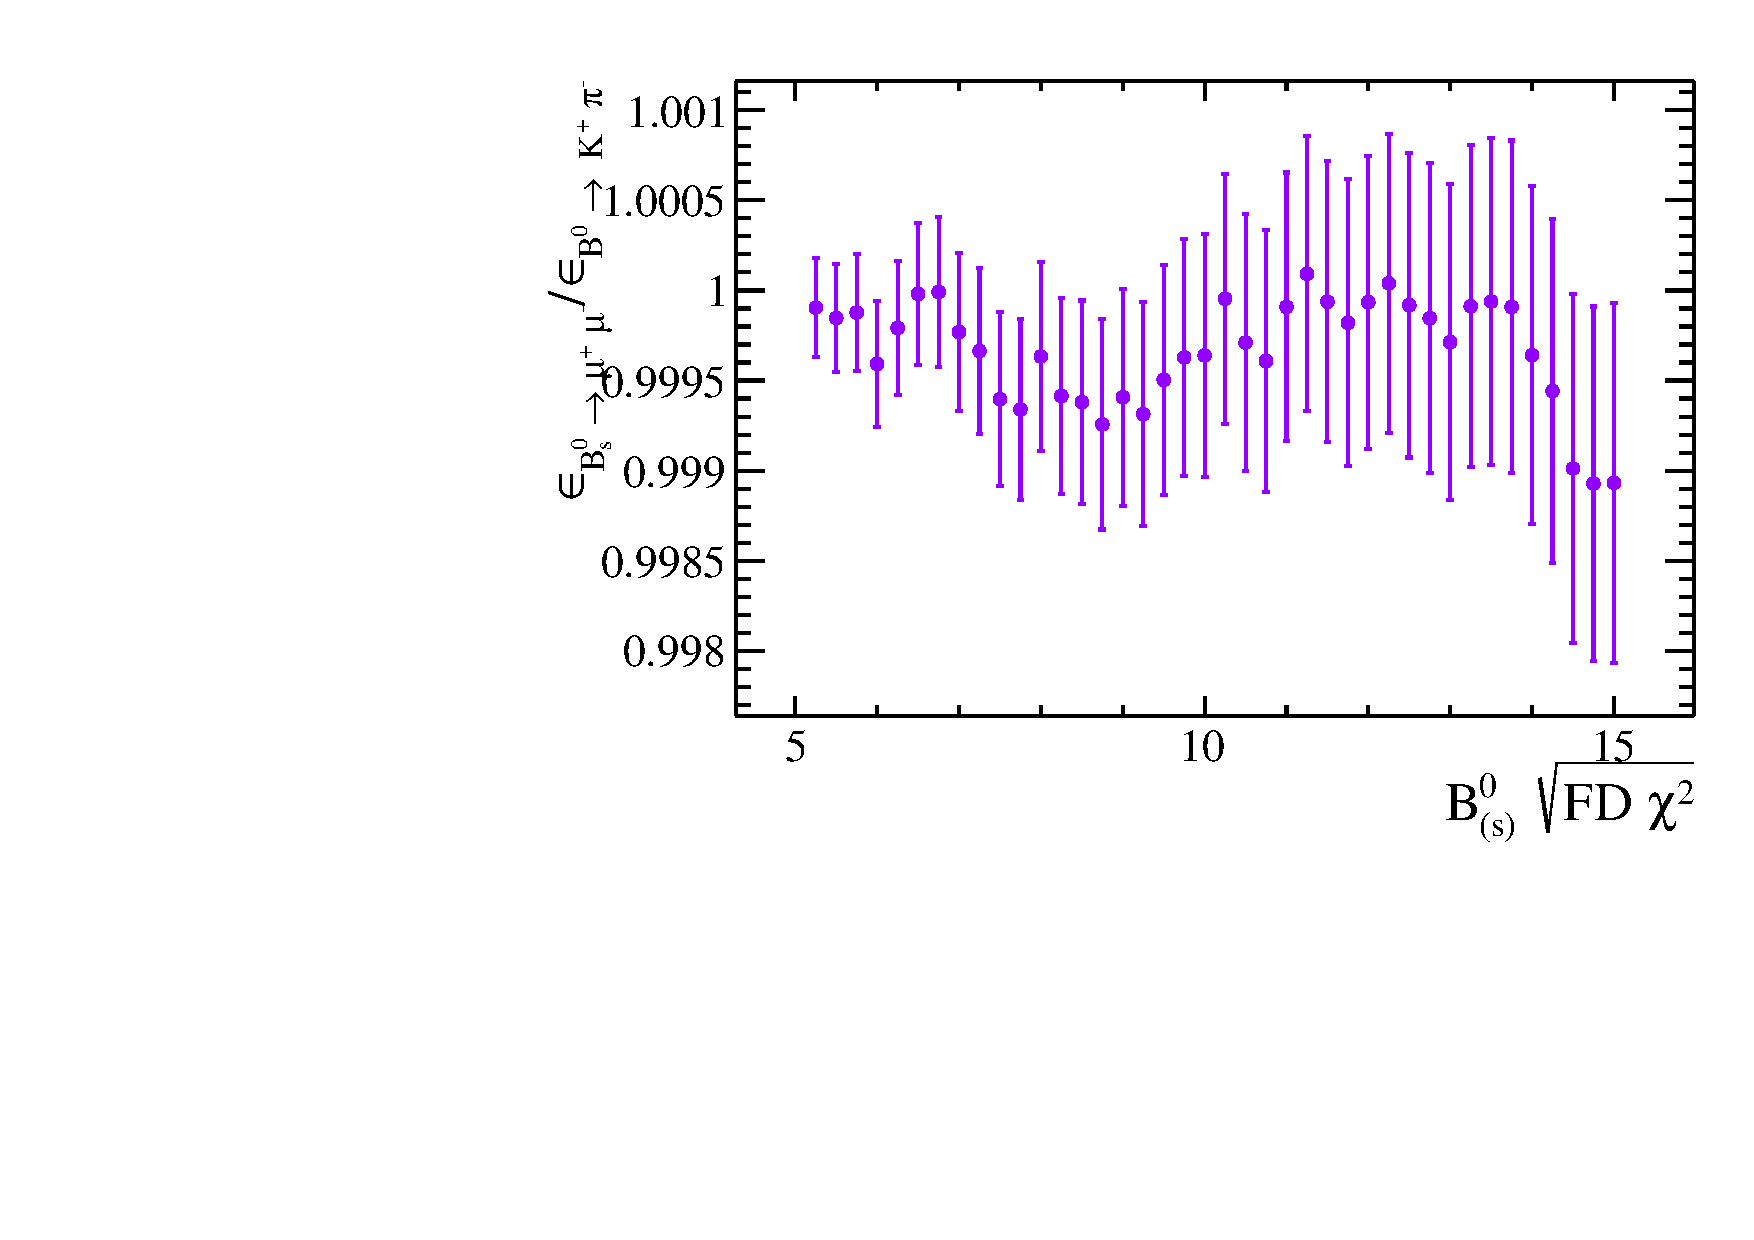
\includegraphics[width=\textwidth]{./Figs/Selection/Bs2MuMu_KPi_FD.pdf}
        %\caption{ }
        %\label{fig:FD_ratioKPi}
    \end{subfigure}
   \begin{subfigure}[b]{0.4\textwidth}
        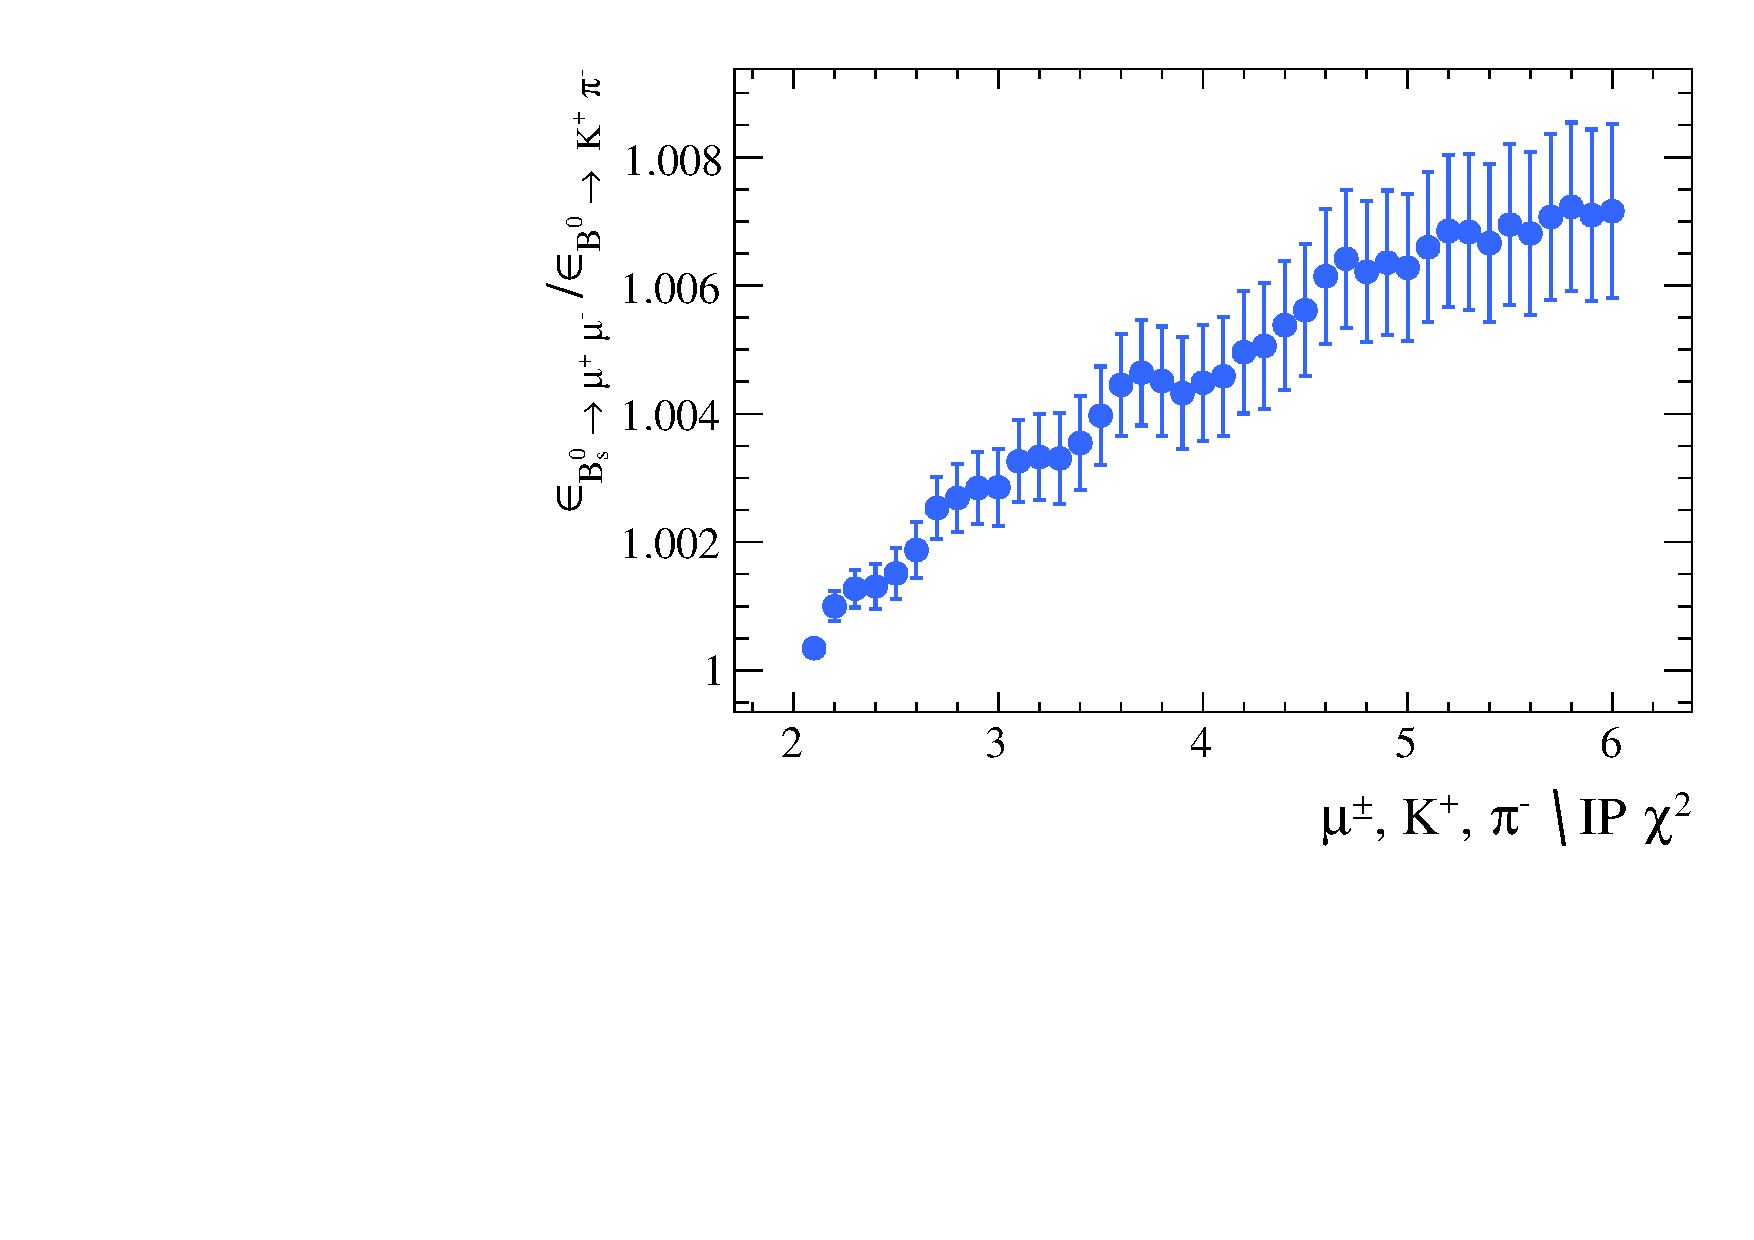
\includegraphics[width=\textwidth]{./Figs/Selection/Bs2MuMu_KPi_daughter_IP.pdf}
        %\caption{ }
        %\label{fig:IPS_ratioKPi}
    \end{subfigure}
    \caption{The ratio of \bsmumu to \bdkpi stripping efficiencies when each cut has been applied independently of all other cuts. The current cut values are marked by the blue lines.}
    \label{fig:ratio_plotsBd2KPi}
\end{figure}


\begin{figure}[htbp]
    \centering
    \begin{subfigure}[b]{0.4\textwidth}
        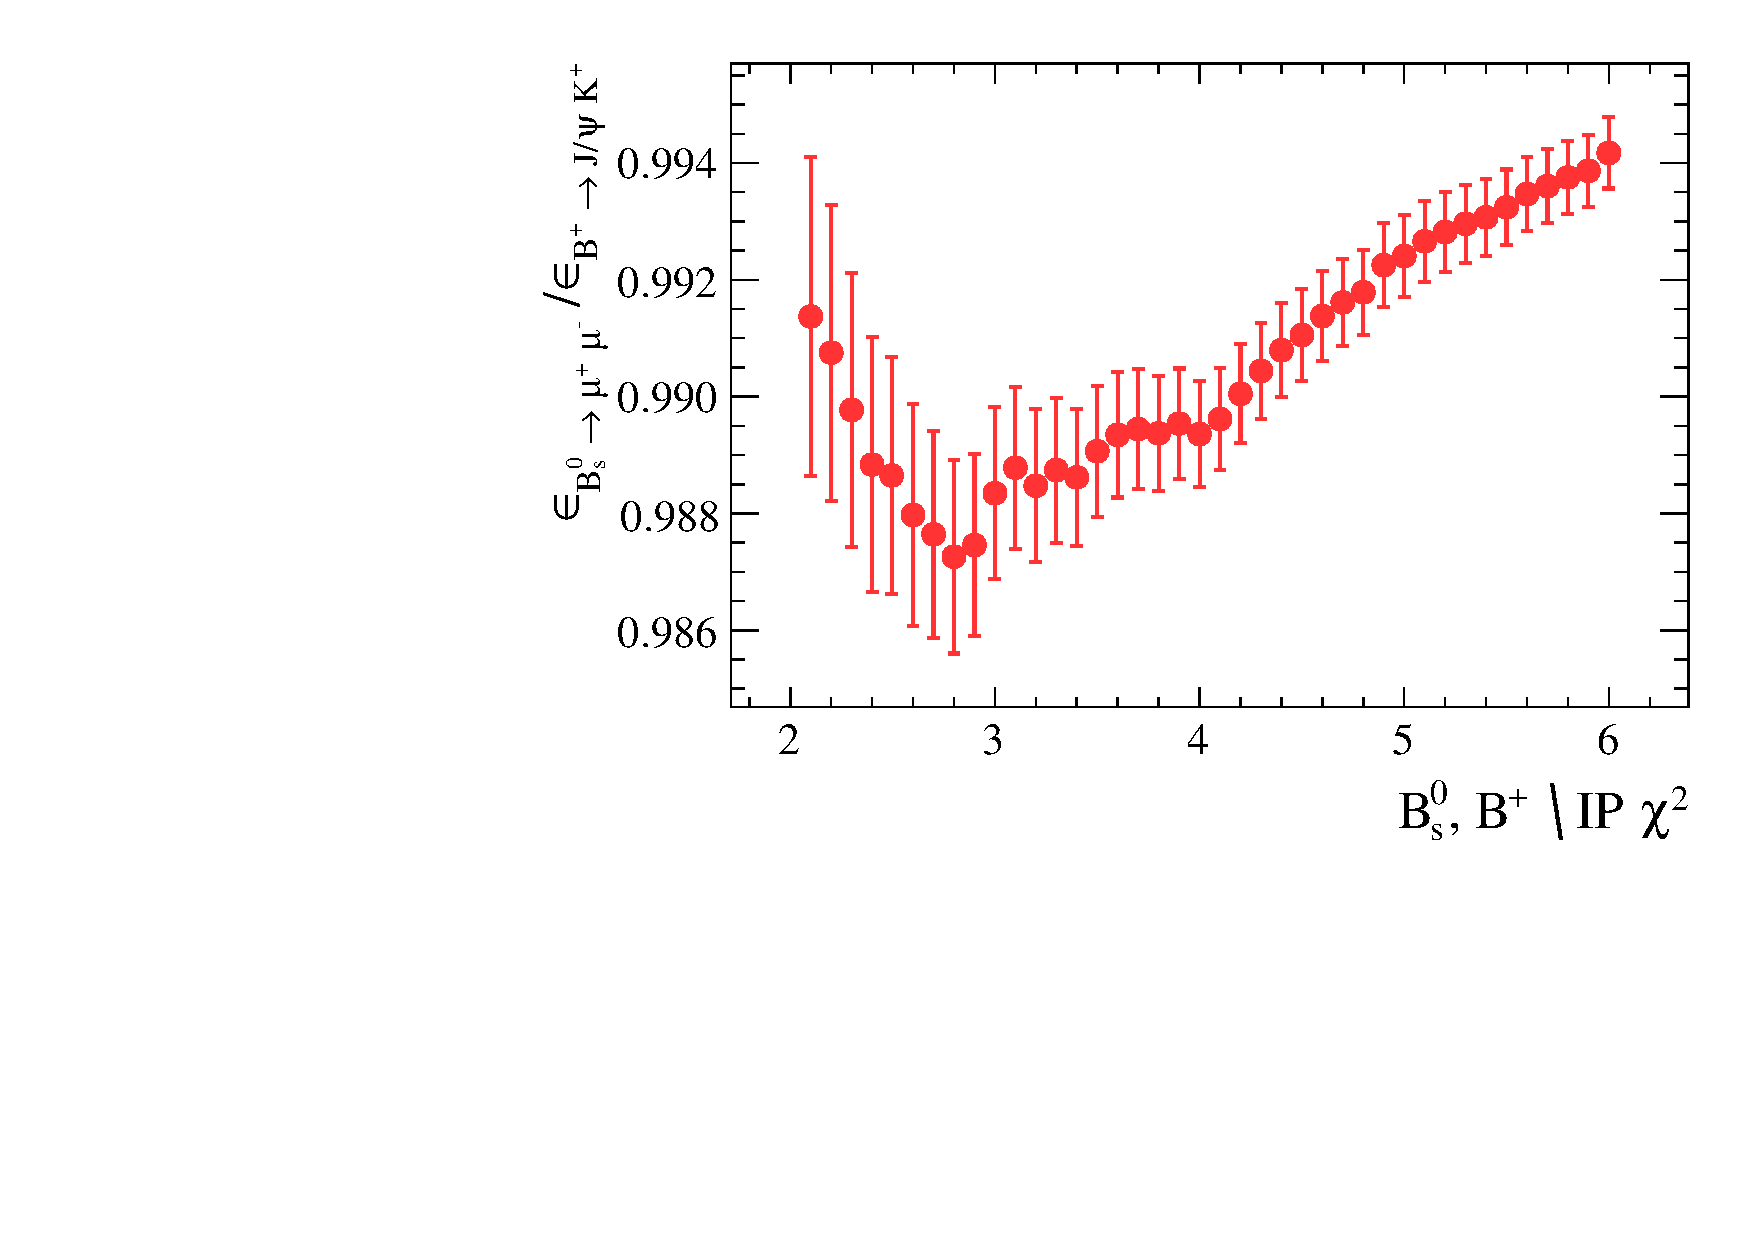
\includegraphics[width=\textwidth]{./Figs/Selection/BsMuMu_JPsiK_IP.pdf}
        %\caption{ }
        %\label{fig:IPS_ratio}
    \end{subfigure}
    ~ %add desired spacing between images, e. g. ~, \quad, \qquad, \hfill etc. 
      %(or a blank line to force the subfigure onto a new line)
    \begin{subfigure}[b]{0.4\textwidth}
        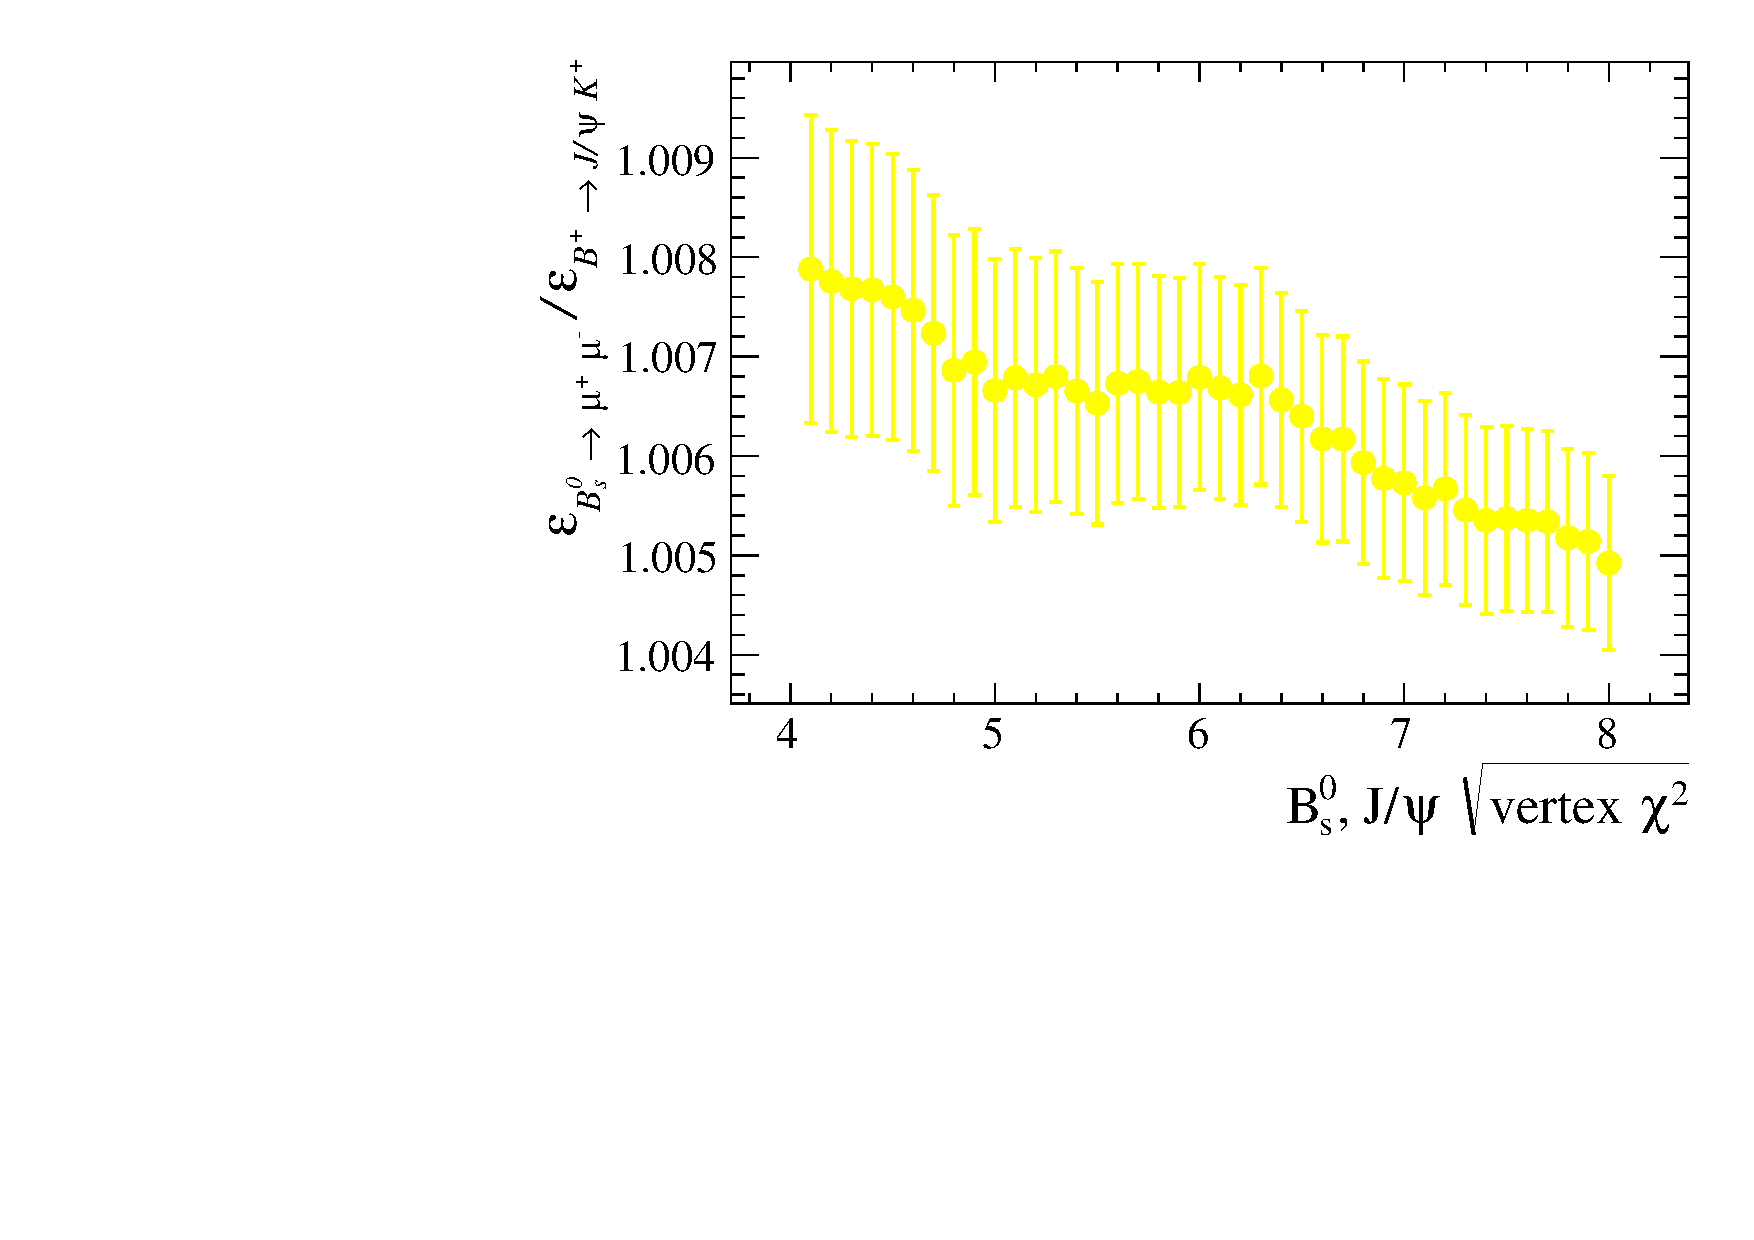
\includegraphics[width=\textwidth]{./Figs/Selection/BsMuMu_JpsiK_vertex.pdf}
        %\caption{ }
        %\label{fig:CHI2_ratio}
    \end{subfigure}
    ~ %add desired spacing between images, e. g. ~, \quad, \qquad, \hfill etc. 
    %(or a blank line to force the subfigure onto a new line)

    \begin{subfigure}[b]{0.4\textwidth}
        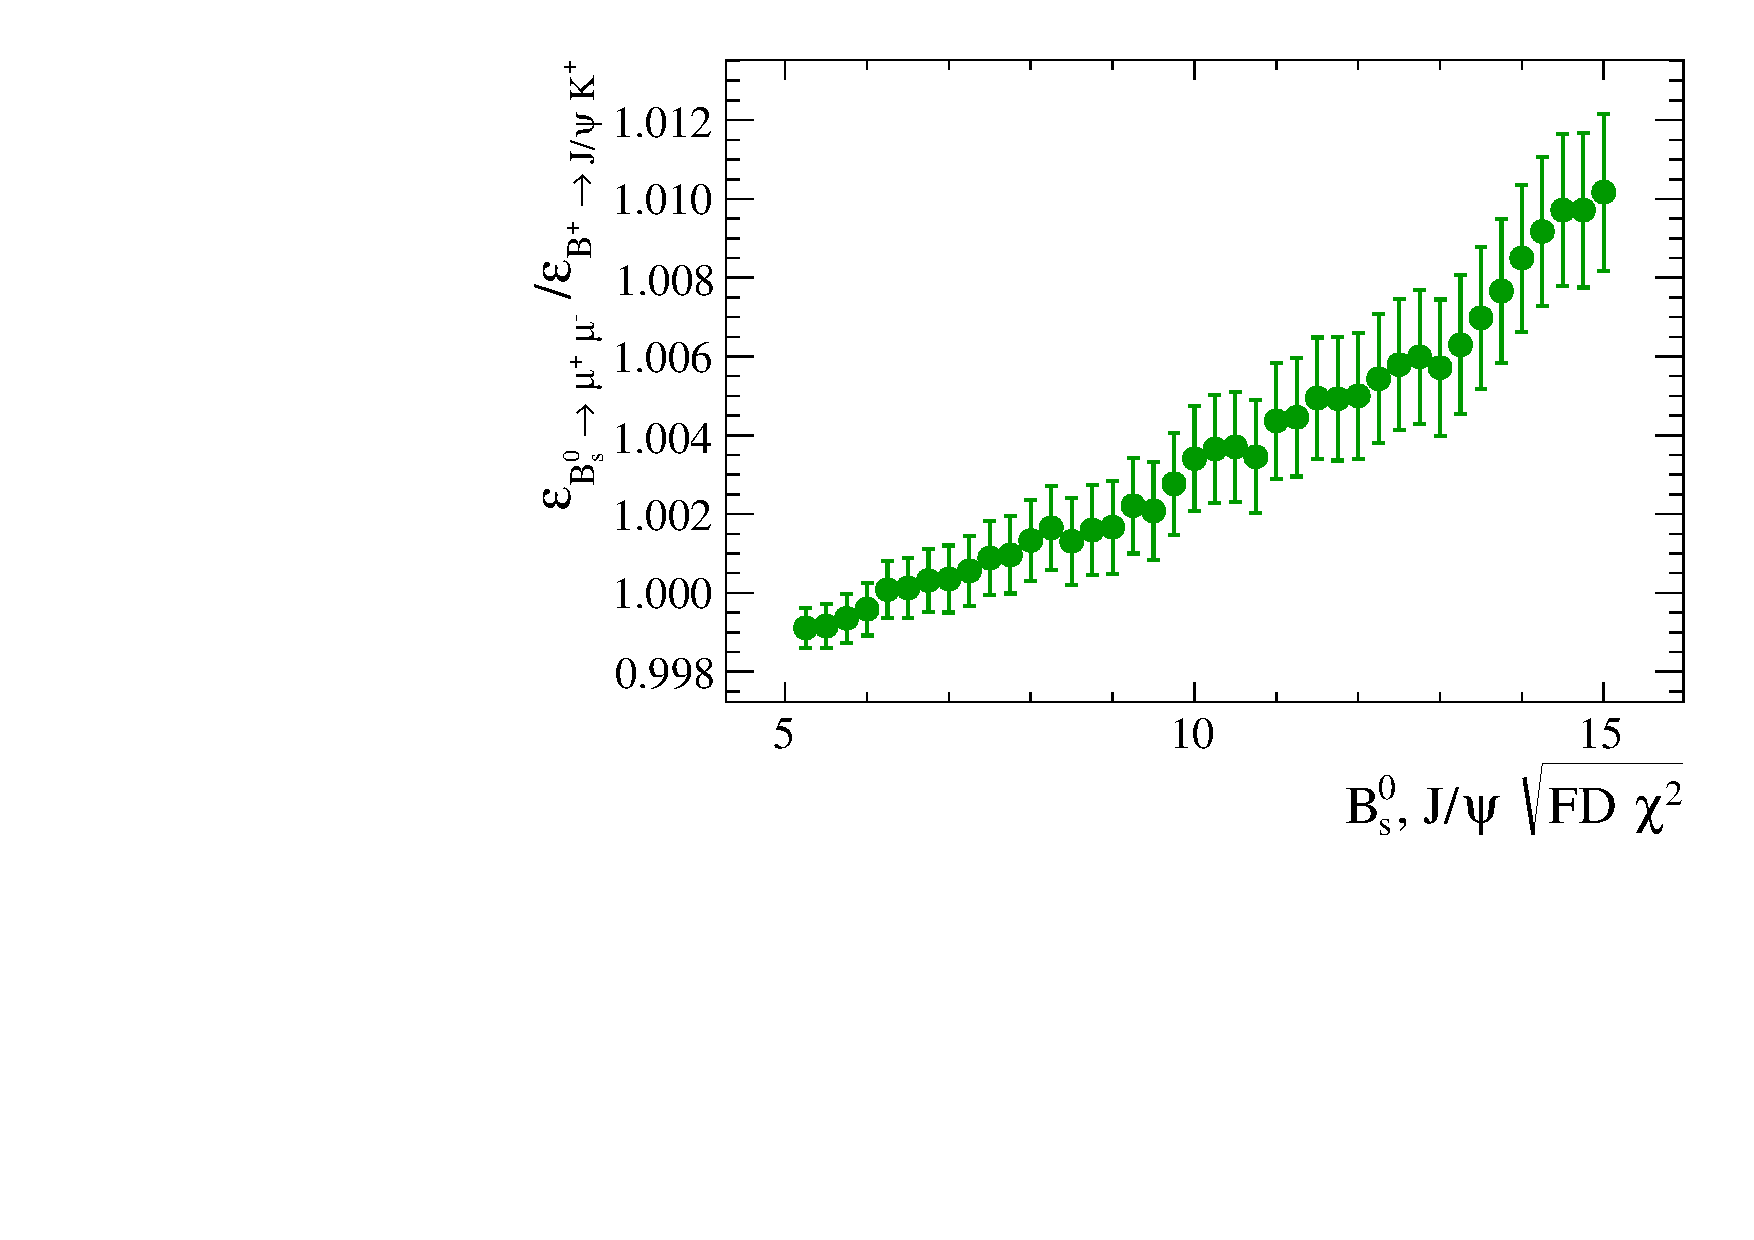
\includegraphics[width=\textwidth]{./Figs/Selection/BsMuMu_JpsiK_FD.pdf}
        %\caption{ }
        %\label{fig:FD_ratio}
    \end{subfigure}
   \begin{subfigure}[b]{0.4\textwidth}
        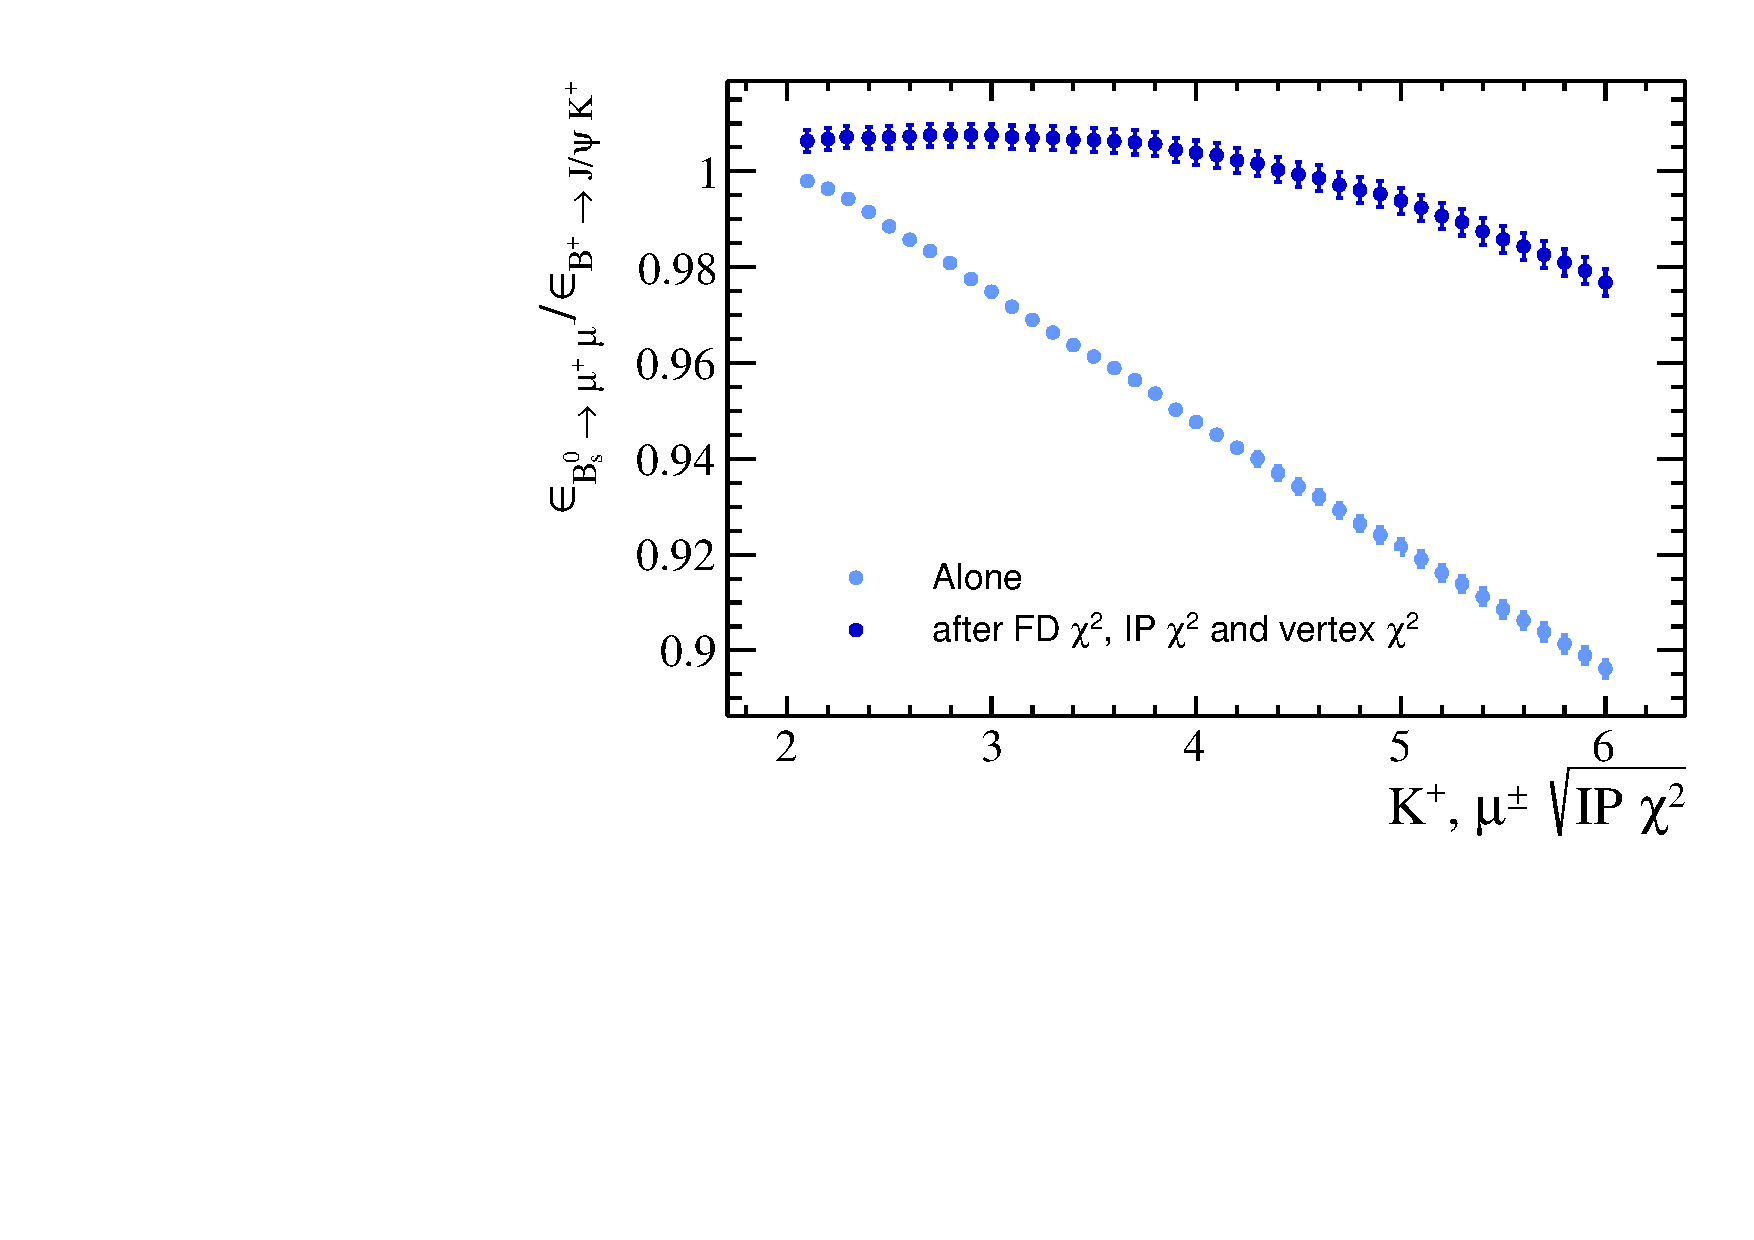
\includegraphics[width=\textwidth]{./Figs/Selection/Bs2MuMu_JpsiK_daughter_IP.pdf}
        %\caption{ }
        %\label{fig:IPS_ratio}
    \end{subfigure}
    \caption{The ratio of $B^{0}_{(s)}\to\mu^{+} \mu^{-}$ to $B^{+}\to J/\psi K^{+}$ stripping efficiencies when each cut has been applied independently of all other cuts. The current cut values are marked by the blue lines.}
    \label{fig:ratioplotsJpsik}
\end{figure}


The efficiencies for most of the stripping cuts as $\sim 97 \%$ or higher, however, the efficiencies of the cuts on the FD $\chi^{2}$ of the \bsd or \jpsi and the daughter IP $\chi^{2}$ of the muon or hadron pair are lower at $83 \%$ and $80 \%$, respectively. Therefore improvements to the stripping selection efficiencies could be achieved by altering these two selection requirements. 



The set of events removed by each cut in the stripping selection is not independent. Therefore the effect of changing one cut on the total efficiency of a stripping selection must be considered. Figure~\ref{fig:efficiencyplots} shows the total efficiency of the \bsmumu stripping line on simulated \bsmumu decays for a range of FD $\chi^{2}$ and daughter IP $\chi^{2}$ cut values. As expected the lower the cut values the more efficient the stripping line becomes. It is important that any increase in \bsmumu selection efficiency from the stripping is not removed when the trigger requirements are applied, Figure~\ref{fig:triggereffplots} shows that the trigger efficiencies are relatively flat across a large range of FD $\chi^{2}$ and daughter IP $\chi^{2}$ cut values therefore the efficiency gained by a change in the stripping selection is not lost when trigger requirements are imposed. The selection efficiency for \bdmumu is very similar to \bsmumu as seen in Table~\ref{tab:Run1strippingEff}, therefore only \bsmumu have been studied for different stripping selection cut values. 


\begin{figure}[htbp]
    \centering
    %\begin{subfigure}[b]{0.4\textwidth}
        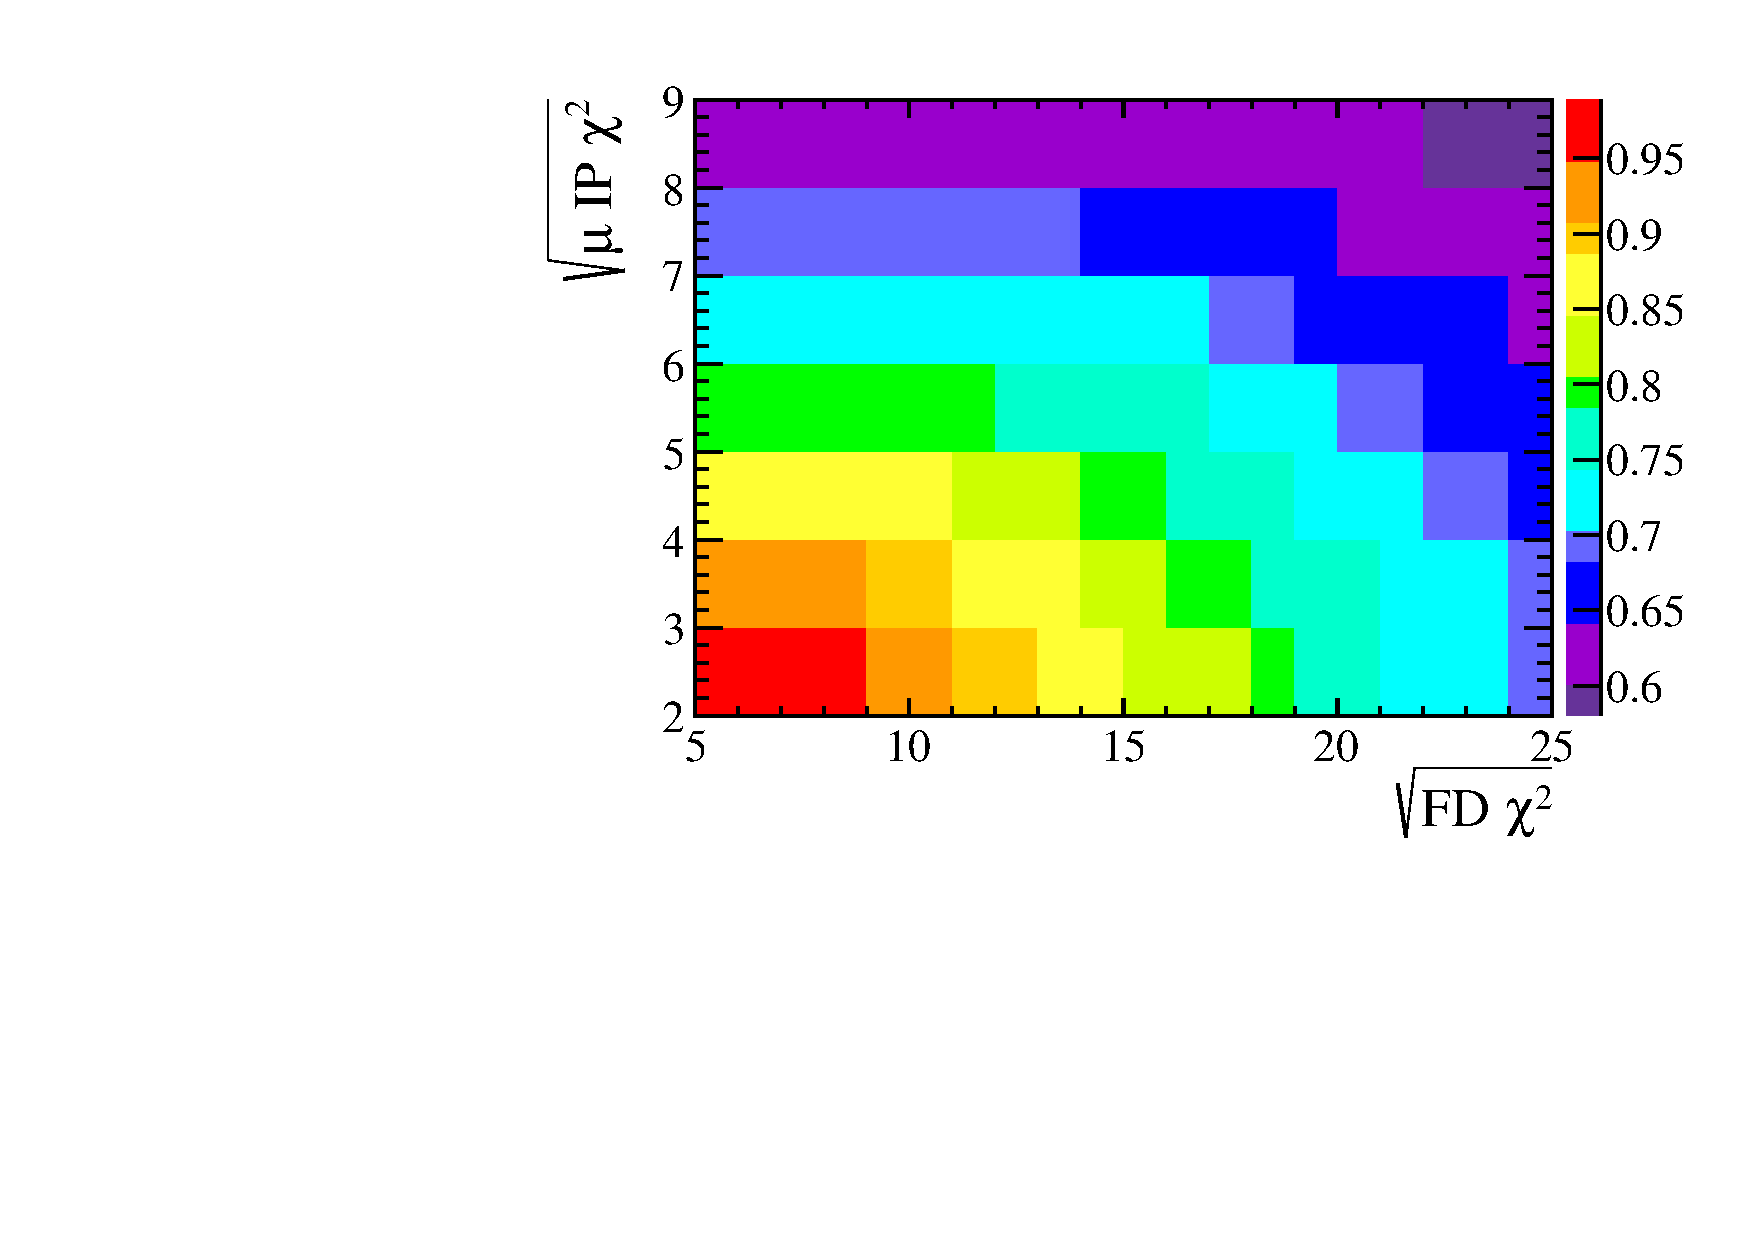
\includegraphics[width= 0.8 \textwidth]{./Figs/Selection/Bs2MuMu_efficiency_chart_Feb3.pdf}
       % \caption{ }
      %  \label{fig:eff}
  %  \end{subfigure}
    ~ %add desired spacing between images, e. g. ~, \quad, \qquad, \hfill etc. 
      %(or a blank line to force the subfigure onto a new line)
   % \begin{subfigure}[b]{0.4\textwidth}
       % 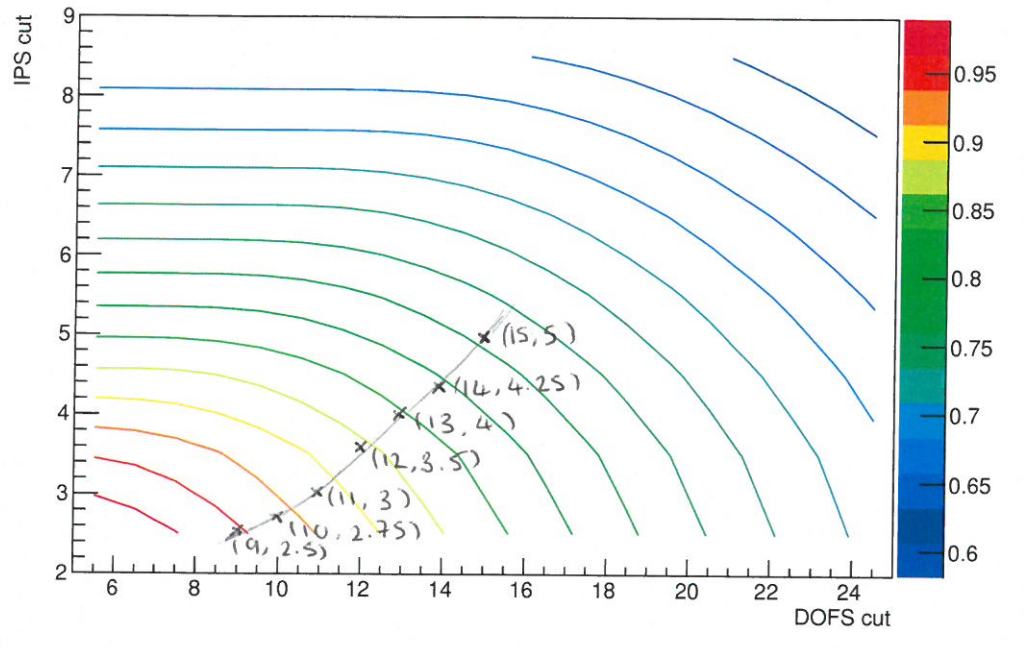
\includegraphics[width=\textwidth]{./Figs/Selection/strip_chart1.png}
      %  \caption{ }
      %  \label{fig:eff_contours}
  %  \end{subfigure}
    \caption{Efficiency of the \bmumu stripping selection for \bsmumu simulated decays for a range of cuts on the \bs FD \chisqd and the minimum muon IP \chisqd.}
    \label{fig:efficiencyplots}
\end{figure}

\begin{figure}[htbp]
   \centering
   % \begin{subfigure}[b]{0.7\textwidth}
   %     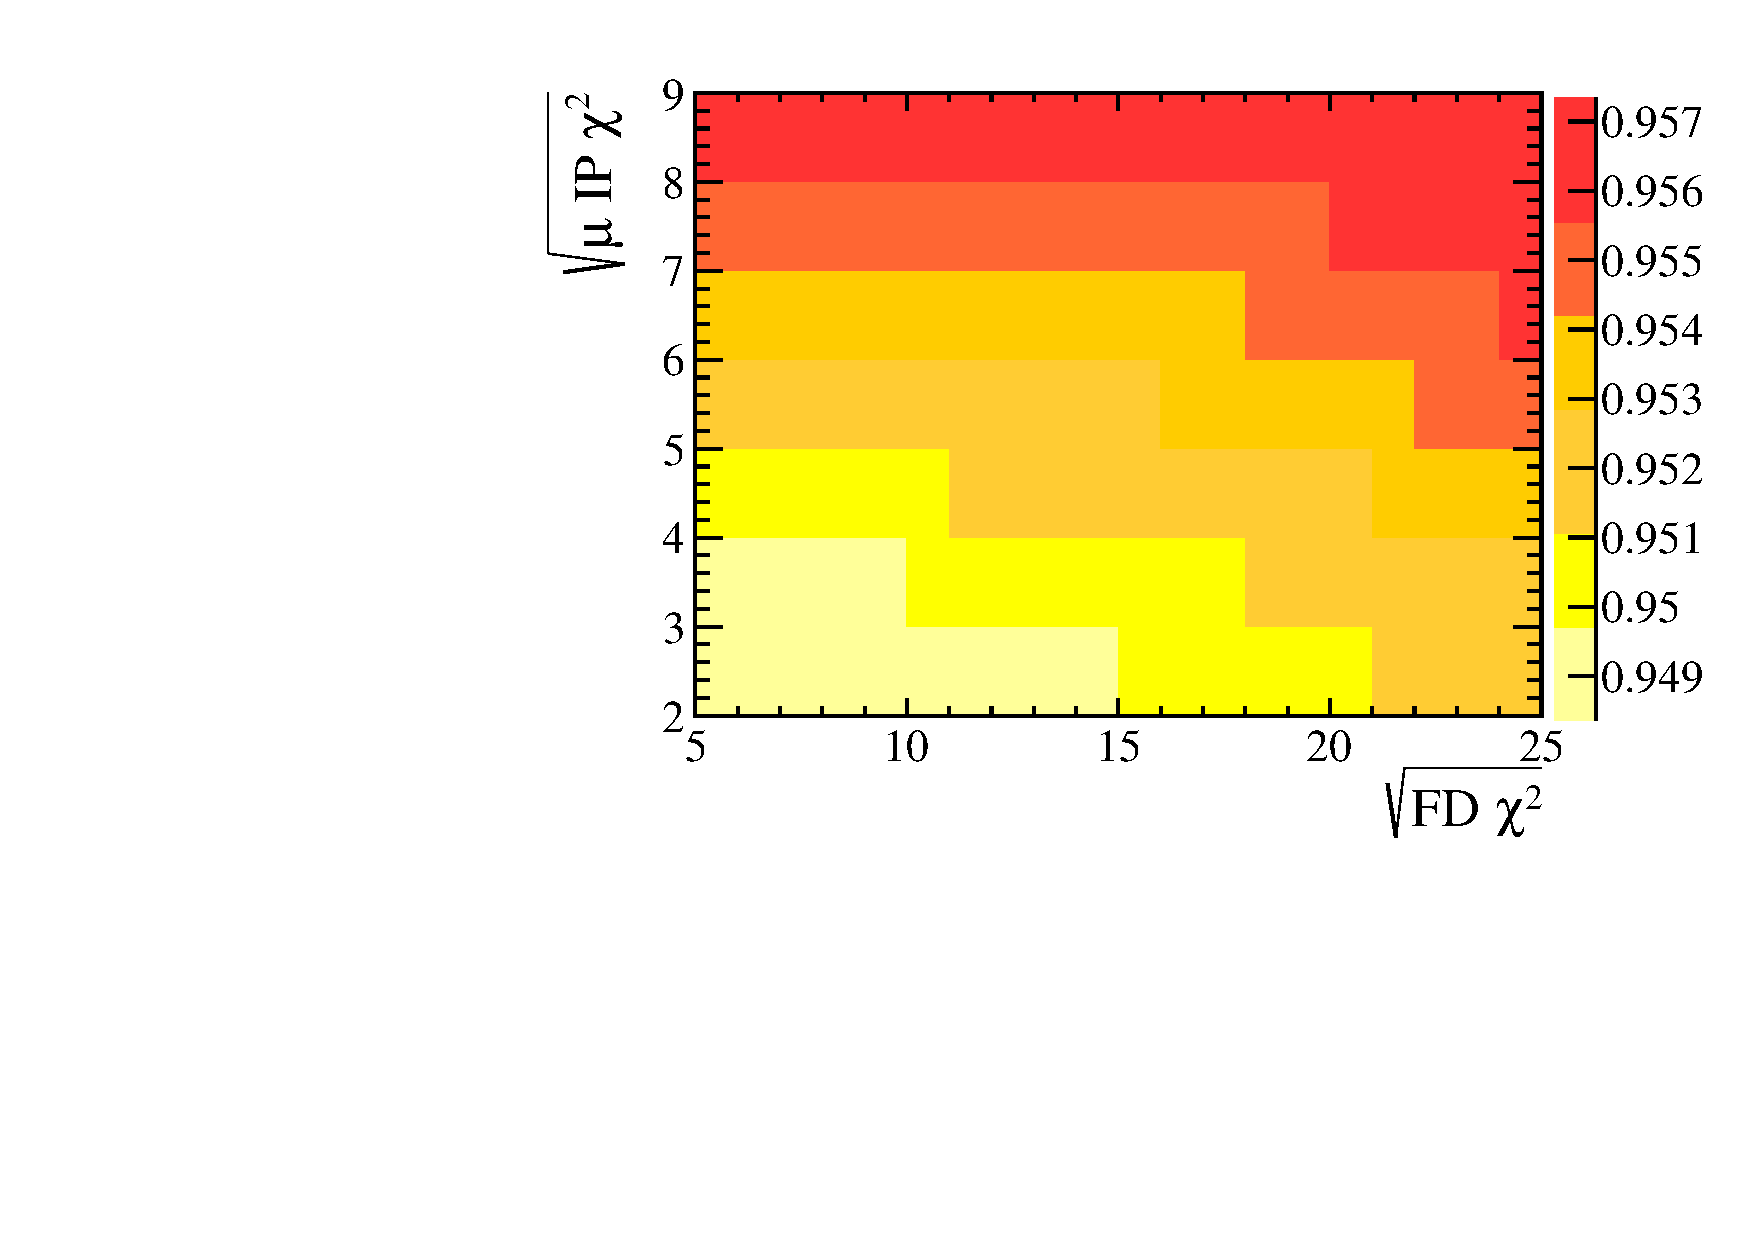
\includegraphics[width=\textwidth]{./Figs/Selection/TIS_TOS_Trigger_chart.pdf}
   %     \caption{ }
   %     \label{fig:TISTOS}
   % \end{subfigure}
   % ~ %add desired spacing between images, e. g. ~, \quad, \qquad, \hfill etc. 
      %(or a blank line to force the subfigure onto a new line)
  %  \begin{subfigure}[b]{0.7\textwidth}
        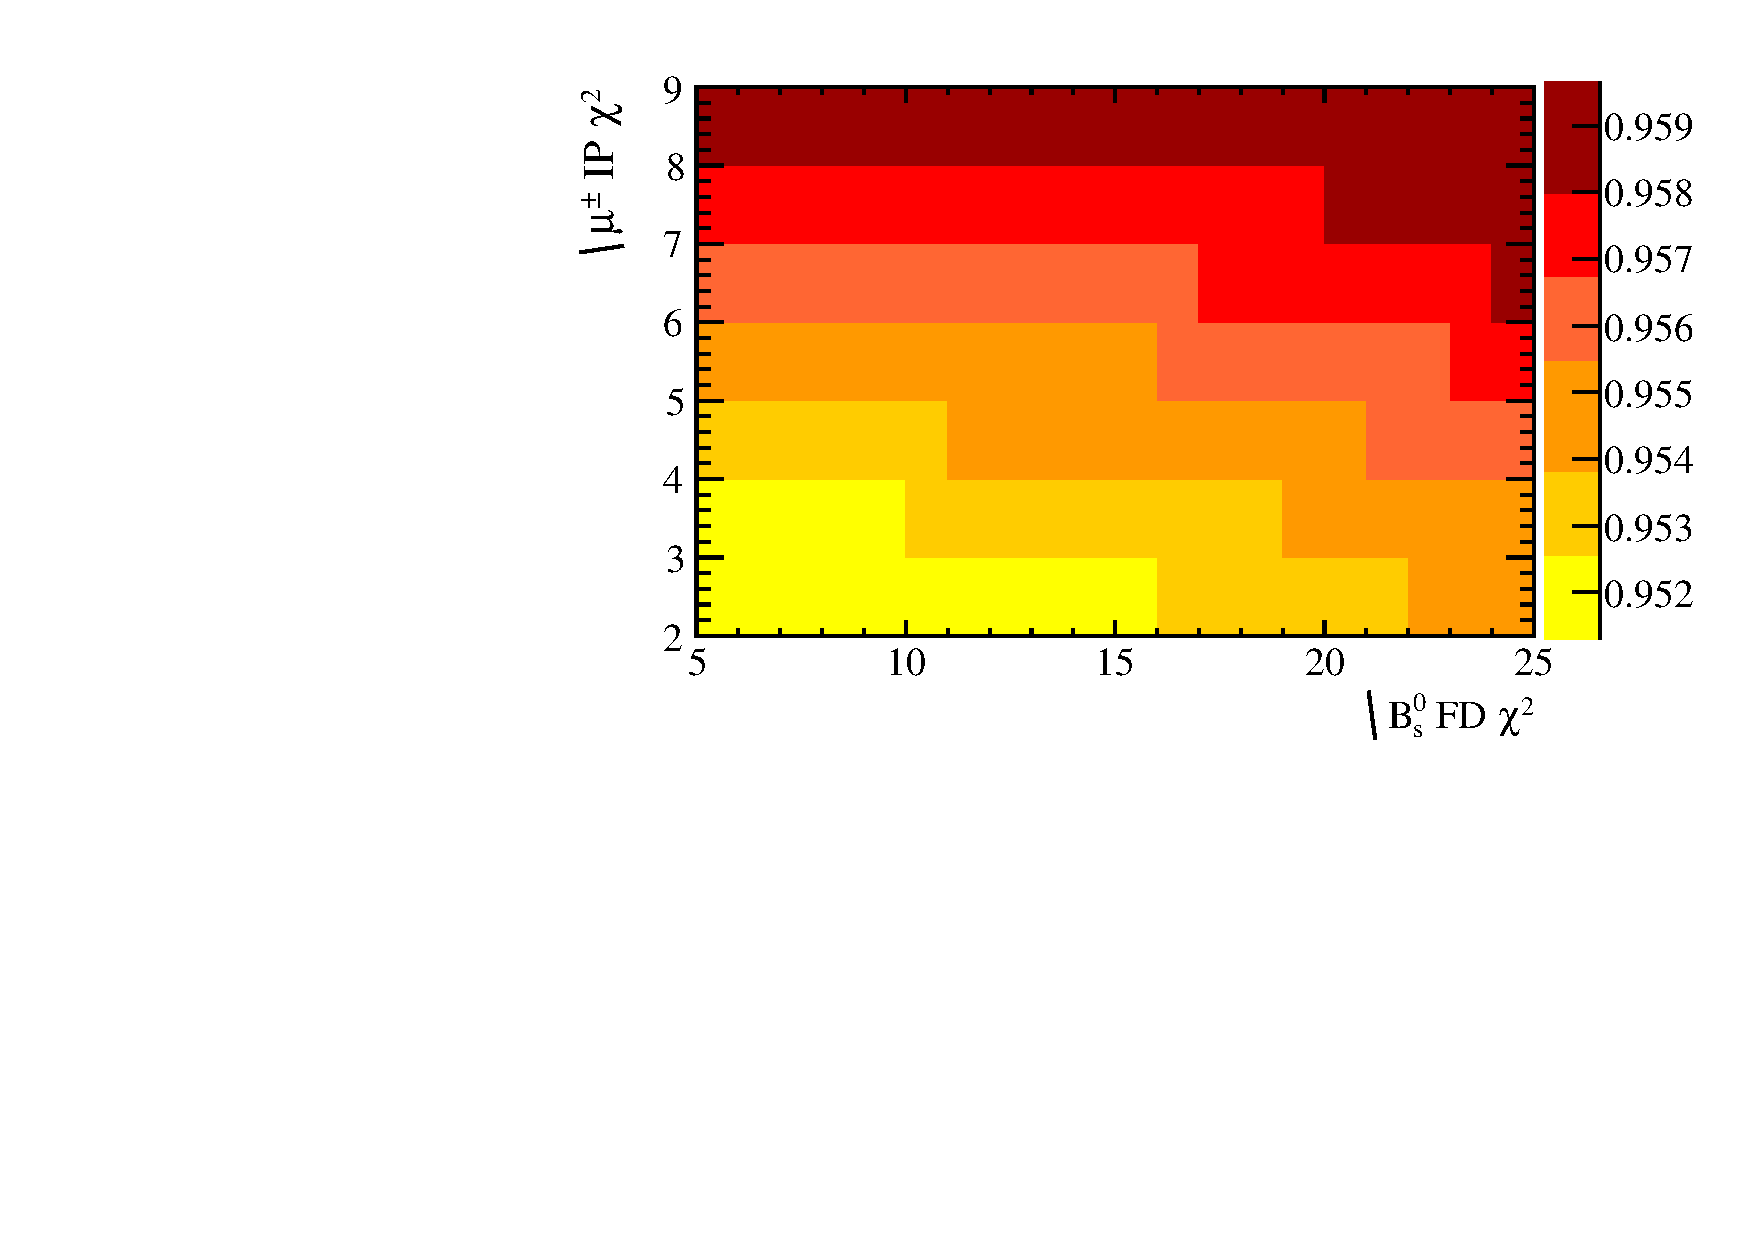
\includegraphics[width=0.8\textwidth]{./Figs/Selection/Dec_trigger_chart.pdf}
   %     \caption{ }
   %     \label{fog:Dec}
   % \end{subfigure}
    \caption{The trigger efficiencies of \bsmumu simulated decays across a range of \bs FD \chisqd and the minimum muon IP \chisqd cut values for the trigger requirements used to select \bmumu decays for the branching fraction measurement. }
    \label{fig:triggereffplots}
\end{figure}





One of the main purposes of the stripping selection, as described in Section~\ref{SoftwareSimulation}, is to reduce the size of the data set, therefore the cuts cannot be set as loose as possible. 

Any change applied to the \bmumu stripping line must be propagated through into the stripping lines for \bhh, \bujpsik and \bsjpsiphi decays therefore the retention of all stripping lines must be evaluated.

Table~\ref{tab:Retention} shows the total efficiency of the \bsmumu stripping line along side the amount of data retained for the set of cuts on the FD \chisqd and daughter IP \chisqd for the \bmumu, \bhh, \bujpsik and \bsjpsiphi stripping lines. The set of chosen cuts aims to keep both cuts as high as possible for a certain \bsmumu efficiency. 



\afterpage{
\begin{landscape}
\vspace*{\fill}
\begin{table}[htbp]
\begin{center}
\begin{tabular}{ cc|c|cccc}\hline
  \multicolumn{2}{c}{Stripping cut}                   & Stripping line efficiency &  \multicolumn{4}{c}{Stripping line retention} \\
\hline
$\sqrt{\text{FD} \chisqd}$ & Daughter  $\sqrt{\text{IP} \chisqd}$ & \bsmumu  & \bmumu & \bdkpi & \bujpsik & \bsjpsiphi \\
\hline
15                    &5.00                  & (71.29 $\pm$ 0.07) $\%$  &  1.0      &1.0     &1.0      & X\\
14                    &4.25                  & (74.91 $\pm$ 0.07) $\%$  &  1.5      &1.3     &1.1      & X \\
13                    &4.00                  & (76.84 $\pm$ 0.07) $\%$  &  1.8      &1.5     &1.2      & X \\
12                    &3.50                  & (79.76 $\pm$ 0.07) $\%$  &  2.6      &1.8     &1.3      & X \\
11                    &3.00                  & (82.72 $\pm$ 0.06) $\%$  &  3.7      &2.4     &1.6      & X \\
10                    &2.75                  & (84.86 $\pm$ 0.06) $\%$  &  4.7      &3.0     &1.7      & X \\
9                     &2.50                  & (86.96 $\pm$ 0.06) $\%$  &  6.8      &3.9     &2.0      & X \\
\hline
\end{tabular}
\end{center}
\label{tab:Retention}
\vspace{0.7cm}
\caption{The efficiency of the \bmumu stripping line to select \bsmumu decays and the changing in the date retention for \bmumu, \bhh, \bujpsik and \bsjpsiphi stripping lines for a range of FD \chisqd and daughter IP \chisqd cut values. Fractional uncertainty on the retention is less than 1 $\%$.}
\end{table}
\vspace*{\fill}
\end{landscape}
}


The data retention is computed by applying the stripping selection to a sub-set of 2012 data to find the number of events that pass the stripping lines for each pair of FD $\chi^{2}$ and daughter IP $\chi^{2}$ cuts. No trigger requirements are imposed on trigger lines because the stripping selection run on the full output of the trigger. The number of events for each set of cuts is normalised to the number of events passing the original Run~1 stripping line requirements  to show the fractional increase caused by loosening the cut values. 

An increase of 15~$\%$ can be gained in the stripping selection efficiencies by using the loosest cuts in Table 3.5 %\ref{tab:Retention} 
however the loosest cuts increases the amount of data passing the \bmumu stripping selection by a factor of 7 and the \bhh stripping selection by a factor of 4. Table~\ref{tab:NumEvents} shows the number of Run~1 candidates passing the original stripping selection listed in Table~\ref{tab:PreviousStripping} for the last published analysis. The \bhh stripping line lets through the most candidates where as the \bmumu stripping line saves far fewer candidates, therefore a chance in the retention of the \bhh line is more significant than the \bmumu line. 


The final set of cuts used in the stripping selection must be a compromise between the selection efficiency and the amount of data that passes the selection. The selection cuts of \bs FD $\chi^{2}$ $>$ 121 and minimum muon IP $\chi^{2}$ $>$ 9 would increase the \bmumu selection efficiency by from 71~$\%$ to 82~$\%$ and the amount of data retained would be doubled. The increase of the data retained by the \bhh, \bujpsik and \bsjpisphi lines is smaller and the efficiencies are similar to the \bmumu selection efficiencies. Therefore these cuts are applied in the stripping selection for this analysis. %However the increase in efficiency after the stripping selection will not necessarily be propagated through the whole analysis. 



\begin{table}[htbp]
\begin{center}
\begin{tabular}{lcc}
\hline
Stripping Lines & Events & Retention / $\%$ \\
\hline
\bmumu & 898880 & 0.0022 \\
\bhh & 14502295  &  0.0831 \\
\bujpsik & 3344568 & 0.0087  \\
\bjpsiphi & 456787  & 0.0011 \\
%$B \to J/\psi K^{*}$ &  12574956 & 0.018 \\
\hline
%Total & 31779975& - \\
%Total with correlation & 31402536 \\
Total & 18745743& - \\
\hline
\end{tabular}
\vspace{0.7cm}
\caption{The number of events passing stripping lines used for the \bsmumu analysis from the selection listed in Table~\ref{tab:PreviousStripping} and the percentage of the total LHCb data set that they correspond to. The total does not include correlation between lines, which is expected to be 42 $\%$ between \bmumu and \bhh lines. }
\label{tab:NumEvents}
\end{center}
\vspace{-1.0cm}                                                                                   
\end{table}





\subsubsection{Additional offline cuts}
\label{finalloosesel}
%Change of previous version, have a summary at the end of the section for each decay and here just list the additional cuts that are applied.

Additional selection requirements are applied after the stripping to remove specific backgrounds. A lower bound is placed on the $B$ meson transverse momentum to remove pairs of muons originating from $pp \to p\mu^{+}\mu^{-} p$ decays and a \jpsi veto is used to remove backgrounds from \bcjpsimunu decays. The semi-leptonic \bcjpsimunu decays, where \jpsimumu, contribute to the background of \bmumu decays when a muon from the \jpsi forms a good vertex with the muon from the $B_{c}^{+}$ decay. Due to the high mass of the $B_{c}^{+}$ this could place mis-reconstructed candidates within the \bs mass window. A `\jpsi veto' can be used to remove background events from \bcjpsimunu decays. The veto works by removing events where one muon from the \bmumu candidate combined with any other oppositely charged muon in the event has $m_{\mu^{+}\mu^{-}}$ -$ m_{J/\psi}} < 30$  \mevcc. %The veto has a rejection power of X  $\%$ on \bcjpsimunu events that have passed \bmumu other selection cuts in Table~\ref{tab:fullpreselection} and rejects only  $\%$ of \bmumu signal events. The expected number of \bcjpsimunu events after the full selection can be found in Section~X.   

Furthermore the offline selection of \bmumu decays includes the momentum, ghost track probability and decay time cuts made in the \bhh stripping line, but were absent in the \bmumu stripping line. Also a narrower mass range of 4900 - 6000 \mevcc us imposed to $B_{s}^{0} \to \mu^{+} \mu^{-} \gamma$ backgrounds. The stripping selection for \bmumu decays is kept loose to allow for the study of background decays in data. 

The selection applied to Run~1 and Run~2 data is the same for all variables expect the track ghost probability and track \chisqd/$ndof$. Slightly looser cuts of track ghost probability $<$ 0.4 and track \chisqd/$ndof$ < $4$, are used for Run~2 to take advantage to changes in the reconstruction that were introduced for Run~2. 

Table~\ref{} summariese all selection cuts used to identify \bmumu, \bhh, \bujpsil and \bsjpsiphi decays at the end of this section.
%The complete list of selection cuts applied in the cut based selection to select \bsmumu and \bhh decays in Run~1 and Run~2 data are listed in Tables~\ref{tab:fullpreselection}. The stripping selection cuts from Table~\ref{tab:PreviousStripping} are included with the $B$ mesons FD \chisqd and daughter IP \chisqd requirements updated to the looser values and the selection of \bmumu decays includes the momentum, ghost track probability and decay time cuts made in the \bhh stripping line, but were absent in the \bmumu stripping line.

%Additional selection requirements are applied after the stripping to remove specific backgrounds. A lower bound is placed on the $B$ meson transverse momentum to remove pairs of muons originating from $pp \to p\mu^{+}\mu^{-} p$ decays and a \jpsi veto is used to remove backgrounds from \bcjpsimunu decays. The semi-leptonic \bcjpsimunu decays, where \jpsimumu, contribute to the background of \bmumu decays when a muon from the \jpsi forms a good vertex with the muon from the $B_{c}^{+}$ decay. Due to the high mass of the $B_{c}^{+}$ this could place mis-reconstructed candidates within the \bs mass window. A `\jpsi veto' can be used to remove background events from \bcjpsimunu decays. The veto works by removing events where one muon from the \bmumu candidate combined with any other oppositely charged muon in the event has $m_{\mu^{+}\mu^{-}}$ -$ m_{J/\psi}} < 30$  \mevcc. %The veto has a rejection power of X  $\%$ on \bcjpsimunu events that have passed \bmumu other selection cuts in Table~\ref{tab:fullpreselection} and rejects only  $\%$ of \bmumu signal events. The expected number of \bcjpsimunu events after the full selection can be found in Section~X. 

%The $B$ meson mass range for both \bsmumu and \bhh decays is narrower than the range in the stripping selection in Section~\ref{strippingold}. \bsmumu candidates are required to have a dimuon invariant mass greater than 5320 \mevcc. The motivation comes from mass fit studies that are detailed in Section X. The consequence of this cut is to remove \bdmumu decays, $B_{s}^{0} \to \mu^{+} \mu^{-} \gamma$ backgrounds and most backgrounds from mis-identified semi-leptonic and \bhh decays. This can be seen from the mass distribution in Figure~\ref{fig:LHCbCMS}. The expect number of \bdmumu and mis-identified decays after the full selection can be found in Section~X. Similarly the \bhh mass window is reduced to remove contributions from mis-identified backgrounds. 

%The selection applied to Run~1 and Run~2 is the same for all variables expect the track ghost probability and track \chisqd/$ndof$. Slightly looser cuts are used for Run~2 to take advantage to changes in the reconstruction that were introduced for Run~2. 

%\begin{landscape}
%\vspace*{\fill}
%\begin{table}[htbp]
%\begin{center}
%\begin{tabular}{lll}
%\hline
%Particle                & \bsmumu                                     & \bhh                                 \\
%\hline
%\bs or $B^{+}$          & 5320 \mevcc $<$ M $<$ 6000 \mevcc           & 5100 \mevcc $<$ M $<$ 5500  \mevcc      \\                          
%                        & DIRA $>$ 0                                    & DIRA $>$ 0                             \\
%                        & FD $\chi^{2}$ $>$ 121                       & FD $\chi^{2}$ $>$ 121                  \\       
%                        & IP $\chi^{2}$ $<$ 25                        & IP $\chi^{2}$ $<$ 25                   \\
%                        & Vertex $\chi^{2}$/ndof $<$ 9                  & Vertex $\chi^{2}$/ndof $<$ 9              \\      
%                        & DOCA $<$ 0.3 mm                             & DOCA $<$ 0.3 mm                          \\    
%                        & $\tau$ $<$ 13.248 \ps                       & $\tau$ $<$ 13.248 \ps                \\
%                        & $p_{T}$ $>$ 500 \mevc                        & $p_{T}$ $>$ 500 \mevc                \\%%

%\hline
%Daughter $\mu$ or $h$   & Track $\chi^{2}$/ndof $<$ 3 (4)               & Track $\chi^{2}$/ndof $<$ 3 (4)         \\                       
%                        & Minimum IP $\chi^{2}$ $>$ 9                 & Minimum IP $\chi^{2}$ $>$ 9           \\             
%                        & 0.25 \gevc $<$ $p_{T}$ $<$ 40 \gevc         & 0.25 \gevc $<$ $p_{T}$ $<$ 40 \gevc    \\
%                        & $p$ $<$ 500 \gevc                             & $p$ $<$ 500 \gevc                       \\
%                        & ghost probability $<$ 0.3 (0.4)             & ghost probability $<$ 0.3 (0.4)   \\
%                        & $|$m_{\mu\mu} - m_{\jpsi}$| $<$ 30$~\mevcc        &$|$m_{\mu\mu} - m_{\jpsi}$| $<$ 30$~\mevcc    \\
%                        & isMuon = True                               &  -                                \\
%
%\hline%

%\hline
%\end{tabular}
%\vspace{0.7cm}
%\caption{Selection cuts applied to select \bsmumu and \bhh decays, where selection is different between Run~1 and Run~2 the Run~2 values are shown in parenthesis.}
%\label{tab:fullpreselection}
%\end{center}
%\end{table}
%\vspace*{\fill}
%\end{landscape}



\subsection{Particle identification}
\label{sec:BFpid}
%Particle identification (PID) variables are used to refine the selection of \bsmumu candidates and to separate different \bhh decays. 

In the selection of \bmumu decays particle identification variables are particularly useful to reduce the backgrounds coming from mis-identified semi-leptonic decays and \bhh decays and also help to reduce the number of combinatorial background events. On top of the isMuon requirement used in the stripping selection, a linear combination of ProbNN variables 
\begin{equation}
\text{PID}_{\mu} = \text{ProbNN}\mu \times(1 -  \text{ProbNN}K)  \times(1 -  \text{ProbNN}p) 
\end{equation}
is used to refine the selection of \bmumu candidates. The ProbNN$K$ variable is effective at removing mis-identified \bhh backgrounds and the ProbNN$p$ variable is effective at removing \lambdab backgrounds that are present under the \bd mass peak. 

Different tunings of the algorithms used in the ProbNN variables are used to select candidates in Run 1 and 2015 data compared to 2016 data. The tunings perform differently therefore the cut values placed on PID$_{\mu}$ are different for each tuning. The cuts applied to data are
\begin{equation}
%\begin{split}
\text{Run 1 and 2015:} \text{ PID}_{\mu} > 0.4 \\
\text{2016:} \text{ PID}_{\mu} > 0.8.
%\end{split}
\end{equation}

The cut value on PID$_{\mu}$ for the Run 1 and 2015 tuning was optimised to sufficently reduce the background decays to enable the highest sensitivity to the \bdmumu because the background decays pollute the \bd mass window. The cut value for 2016 was chosen to have the same or lower background rejection as the Run 1 and 2015 cut, however the 2016 tuning has a better performance therefore the final cut choice has a high efficiency for selecting \bmumu decays. 

%The cut values applied to data are given in Table~\ref{tab:BFPID}} along with the different ProbNN algorithm tunings. %The cut value for 2016 was chosen to have the same or lower background rejection as the Run 1 and 2015 cut and a high efficiency for selecting \bmumu decays. 


%\begin{table}[htbp]
%\begin{center}
%\begin{tabular}{lll}
%\hline
%Year & ProbNN tune & Cut value \\   
%Run 1 and 2015 & MC12TuneV2 & PID$_{\mu}$ > 0.4 \\
%2016 & MC15TuneV1 & PID$_{\mu}$ > 0.8 \\
%\hline
%\end{tabular}
%\vspace{0.7cm}
%\vspace{0.7cm}
%\caption{Particle identification requirements to select \bsmumu decays in Run 1 and Run 2 data. }
%\label{tab:BFPID}
%\end{center}
%\vspace{-1.0cm}
%\end{table}


\subsection{Multivariate Classifiers}
\label{sec:MVC}

The selection described so far removes a large number of background candidates however because \bmumu decays occur very rarely the data is still dominated by long lived combinatorial background from \bbbarmumux decays. To improve the seperation of signal and backgound decays two  multivariate classifiers are used.

A multivariate classifier is an algorithm that learns differences between signal and background decays. The classifier is given two input samples, one contain only signal decays and the other containing just background decays and a set of input variables. These input variables have different distributions for signal and background decays. The classifier uses the distributions of the input variables along with its knowledge of which decays are signal and background to learn the difference between the two types. The algorithm can then be applied to a data set containing an unknown mixture of signal and background decays to separate them. For each decay the algorithm produces a number, typically between -1 and +1, where high numbers indicate signal-like decays and low numbers indicating background-like decays. A cut is placed on the output of the classifier to remove background so that the remaining data set has a higher purity for signal events.

Two multivariate classifiers are used to identify \bsmumu decays. Both classifiers are a type called a Boosted Decision Tree (BDT) that are described in Section~\ref{sec:GeneralBDT}. %A range of different classifiers were investigated but BDTs preformed the best at separating signal from background. 

The first classifier (Sect.~\ref{BDTS}), called the BDTS, is used to remove candidates that are very unlikely to be signal and it has a high efficiency to select \bmumu decays. The second classifier (Sect.~\ref{sec:globalBDT}), called the global BDT, is used to classify candidates into bins containing increasing proportions of signal candidates, no candidates are removed based on the output of the second BDT. The the BDTS is necessary to reduce the number of background events to a more manageable level for the global BDT.

\subsection{Boosted Decision Trees}
\label{sec:GeneralBDT}
A BDT is made up of the combined outputs of separate decision trees. A decision tree begins with a data sample, where each decay is know to be signal or background and a set of variables describing them. The decision tree applies a cut on a variable that will be the most effective at separating the signal and background in the sample and creates two sub-samples. Another cut is then applied to each of the sub-samples to further separate signal from background. This process is repeated until either a certain number of cuts, defined as the depth of the tree, or the number of candidates in each sub-sample has reached a minimum number. Each sub-sample produced at the end of the tree is called a leaf. The tree uses the knowledge of whether decays are signal or background to assign a value of +1 or -1 to every decay. A decay is given a value +1 if it is in a leaf where the majority is signal and the value -1 if it is in a leaf that has a majority of background decays. The final decisions made by the tree are not prefect, some signal (background) decays will be mis-classified as background and given the value of -1 (+1). %The decision making process of a decision tree is illustrated in Figure~\ref{fig:DT}.

%\begin{figure}
 %   \centering
    %\begin{subfigure}[b]{0.4\textwidth}                                                                                                                          
  %      
\includegraphics[width=\textwidth]{./Figs/placeholder.jpeg}
       % \caption{ }                                                                                                                                              
      %  \label{fig:eff}                                                                                                                                          
  %  \end{subfigure}                                                                                                                                              
   % ~ %add desired spacing between images, e. g. ~, \quad, \qquad, \hfill etc.                                                                                    
      %(or a blank line to force the subfigure onto a new line)                                                                                                   
   % \begin{subfigure}[b]{0.4\textwidth}                                                                                                                          
       % 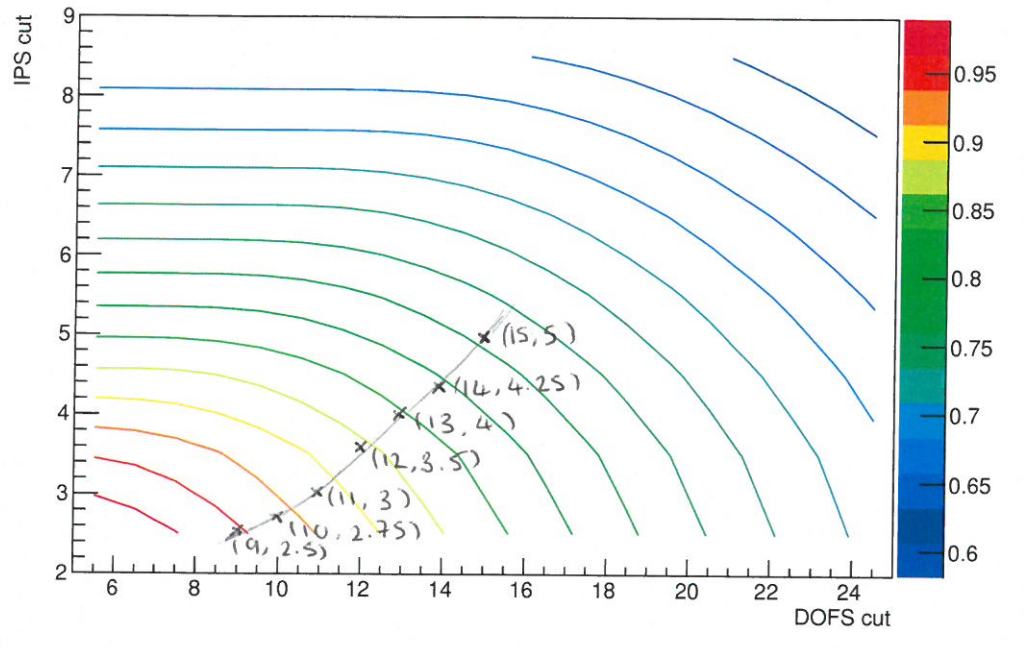
\includegraphics[width=\textwidth]{./Figs/Selection/strip_chart1.png}                                                                                    
      %  \caption{ }                                                                                                                                              
      %  \label{fig:eff_contours}                                                                                                                                 
  %  \end{subfigure}                                                                                                                                              
   % \caption{Illustration of a decision tree.}
   % \label{fig:DT}
%\end{figure}

One decision tree on its own is often not particularly good at classifying events, there is no way to correct mis-classified events in the leaves, and it is particularly sensitive to statistical fluctuations in the training samples. A BDT combines the output of numerous decision trees to improve the classification of events and reduce the dependence of the final decisions on statistical fluctuations. A BDT starts with one decision tree and assigns weights to decays in the signal and background samples depending on whether the output of the decision tree classified the events correctly or incorrectly. The weighted sample is then used as the input for the training of the next decision tree. The weights are designed so that the next tree is more likely to correctly classify previously mis-classified events. This process is repeated until a certain number of trees have been trained. The re-weighting process is known as boosting and the weights applied to the samples are taken into account when combining the output of each decision tree into the overall output of the BDT. The output of a BDT will be a number between -1 and +1 where high numbers indicate signal and low numbers indicating background.


The TMVA package~\cite{Hocker:2007ht} is use to develop and train the BDTs, the package provides several different methods of boosting that can be used. The adaptive boosting method was found to produce the most effective BDT.
This method of boosting assigns decays incorrectly classified by one tree the weight, $w$, before being used as the input to the next decision tree. The weights assigned are given by
\begin{equation}
w = \frac{1 - f}{f}\text{, where } f = \frac{\text{total misclassified events}}{\text{total events}}.
\end{equation}
Therefore incorrectly assigned candidates are given a higher weight than correctly classified candidates. The `speed’ at which the boosting occurs is controlled by a the parameter $\beta$ where $w \rightarrow w^{\beta}$, this can be specified in the training of the decision tree and a large number of boosting steps can improve the performance of the BDT.

The ability of a BDT to correctly identify signal and background candidates depends on three main factors;
\begin{itemize}
\item the size of the training samples - a large training sample is useful to prevent the BDT from being sensitive to statistical fluctuations and contains more information the classifier can use to learn the difference between signal and background
\item the input variables - different distributions in the input variables for signal and background candidates enable the classifier to easily separate the types of candidates, the overall performance is insensitive to poorly discriminating variables that are included
\item parameters that dictate the BDT training - the training of a BDT is specified by several parameters; the number of trees (NTrees), the tree depth (MaxDepth), the minimum number of events a leaf can contain (nEventsMin or MinNodeSize\footnote{nEventsMin is the minimum number of decays in a lead where as MinNodeSize is the number of decays in a leaf given as a percentage of the training sample size. The parameter specified in the training depends on the version of the TMVA package used. });, the `speed’ at which the boosting occurs ($\beta$) and the number of cut values that a tree tries for a variable before making a decision (nCuts).
\end{itemize}

These three factors affect the performance of the BDT however the importance of each varies. Together they can be used to prevent the BDT being very sensitive to the statistical fluctuations in the training sample. This  is called overtraining, an overtrained BDT is extremely accurate at classifying the candidates in the training sample by preforms poorly at classifying candidates in a statistically independent sample. Although this is less common in BDT than single decision trees, it can be avoided by having a sufficiently large training sample or by limiting the depth of trees or the number of trees in the BDT. 

\subsubsection{The BDTS}
\label{BDTS}
%The output of the stripping selection still includes many background decays, further cuts shown in Table~\ref{} reduce the background decays. Some selection cuts are designed to remove specific background decays and the selection for \bsmumu decays used in the Branching Fraction and effective lifetime analyses starts to diverge slightly.

%The BDTS is a multivariate classifier that is designed to reduce the number of combinatorial background events. It is a Boosted Decision Tree (BDT) (see Section~\ref{} for a detailed description) that is trained on \bsmumu and \bbbarmumux simulated decays that have passed the \bmumu selection requirements in Table~\ref{} and additional particle identification cuts listed in Table X. 
The BDTS uses input variables similar to those in the stripping selection to classify events;
\begin{itemize}
\item impact parameter \chisqd of the \bs
\item vertex \chisqd of the \bs
\item direction cosine of \bs
\item distance of closest approach of the muons
\item minimum impact parameter \chisqd of the muons with respect to all primary vertices in the event
\item impact parameter of the \bs, this is the distance of closest approach of the $B$ to the primary vertex
\end{itemize}
The signal and background samples used to train the BDTS are simulated \bsmumu decays and \bsmumu candidates in a sample of Run~1 data from the mass ranges 4800 - 5000 \mevcc and 5500 - 6000 \mevcc. The selection cuts listed in Table~\ref{tab:BDTSpresel} are applied to the training samples and the training parameters used in the BDT are listed in Table~\ref{tab:BDTStrainingparams}. The output of the BDTS is flattened between 0 and 1 so that signal is uniformly distributed across the range and background is peaked at zero as illustrated in Figure~\ref{fig:FlatteningBDTS}. The BDTS is applied to all candidates passing the \bmumum, \bhh and \bujpsik stripping lines, and candidates are required to have a BDTS value above 0.05. When the BDTS is applied to \bujpsik decays the distance of closest approach of the muons refers to the muons in the \jpsi and the vertex \chisq is of the \jpsi. %The chosen cut value has a efficiency of X $\%$ on \bsmumu decays and reject X $\%$ of \bbbarmumux decays. 
The performance of the BDTS at removing backgrounds is illustrated in Figure~\ref{fig:BDTSpreformance}. %Full details of the development of the BDTS can be found in~\ref{}.

\begin{figure}[htbp]
    \centering
    \begin{subfigure}[b]{0.45\textwidth}
        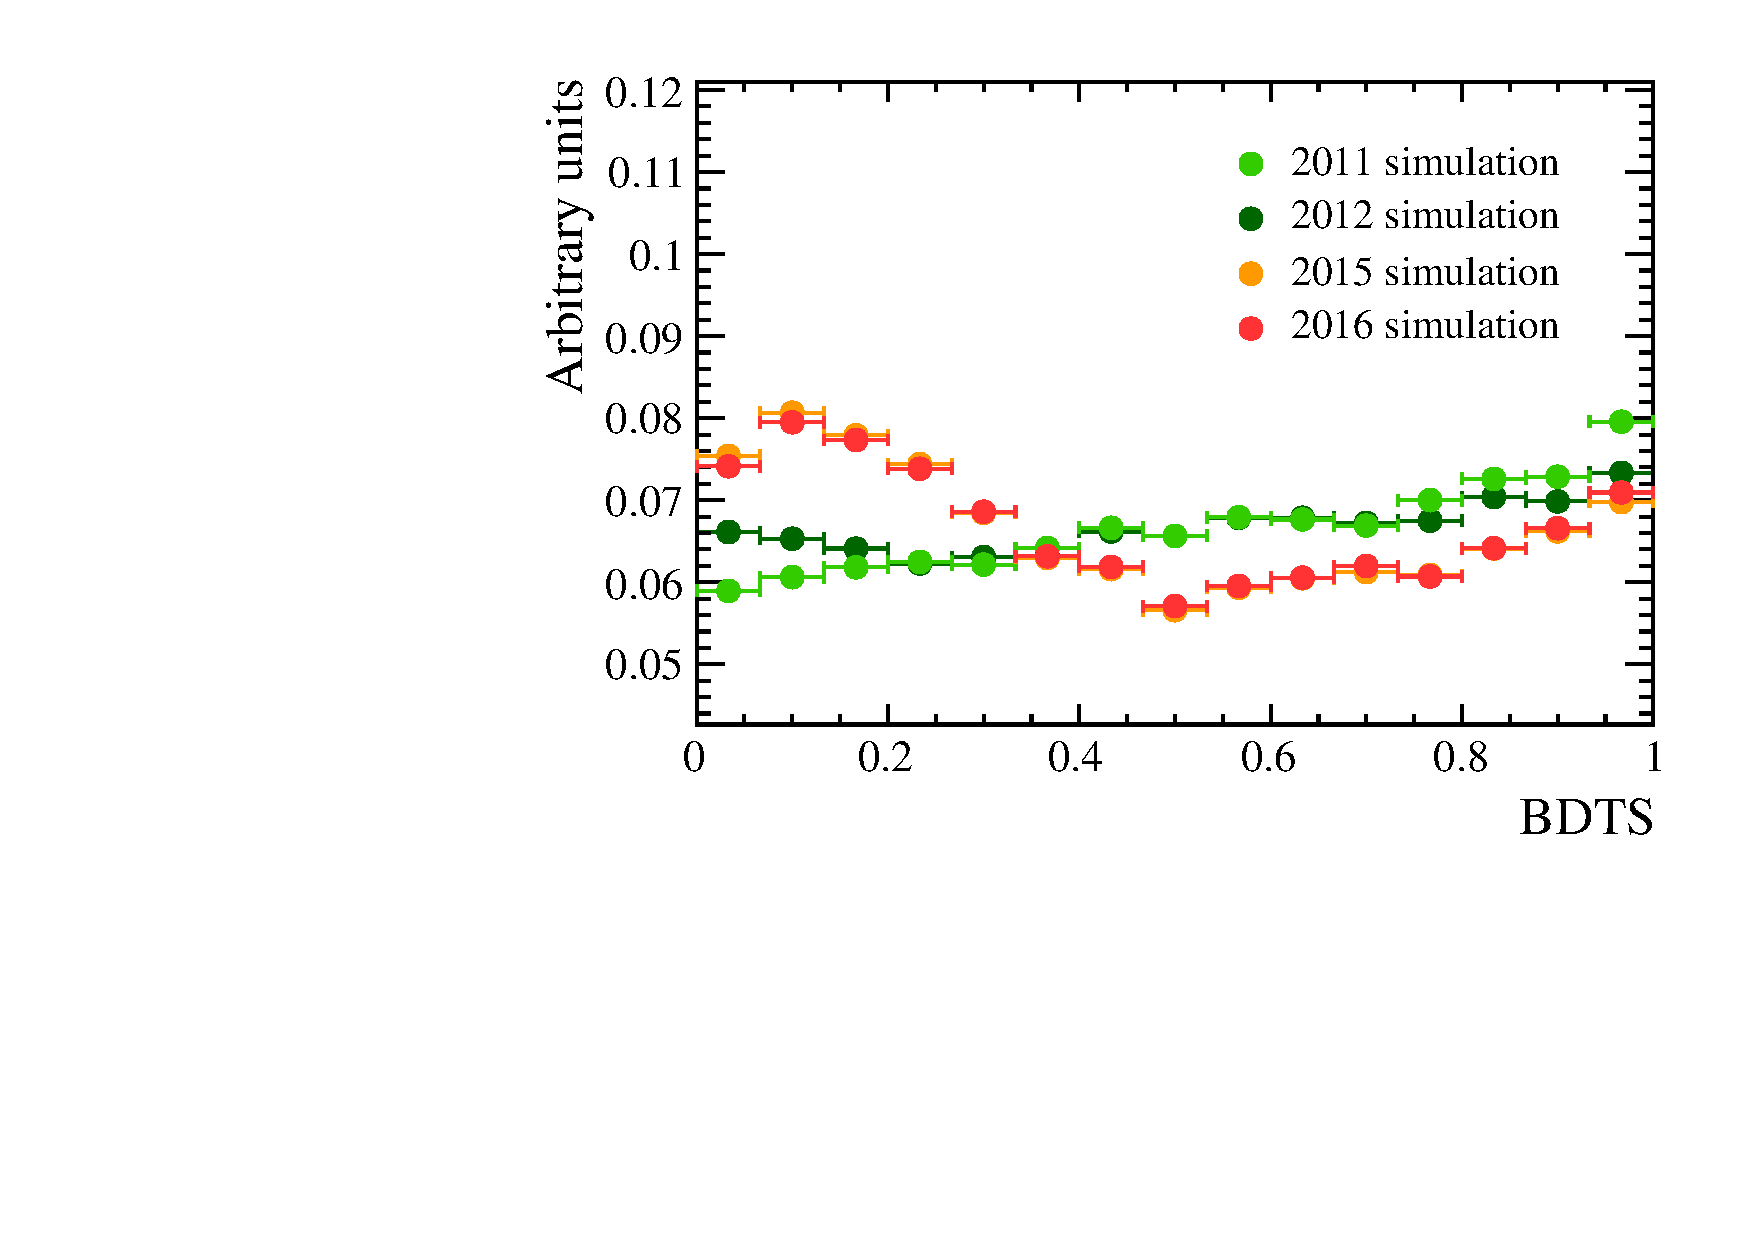
\includegraphics[width=\textwidth]{./Figs/Selection/BDTS_signal_Feb6.pdf}
        %\caption{ }
        %\label{fig:BDTSsig}
    \end{subfigure}
    ~ %add desired spacing between images, e. g. ~, \quad, \qquad, \hfill etc. 
      %(or a blank line to force the subfigure onto a new line)
    \begin{subfigure}[b]{0.45\textwidth}
       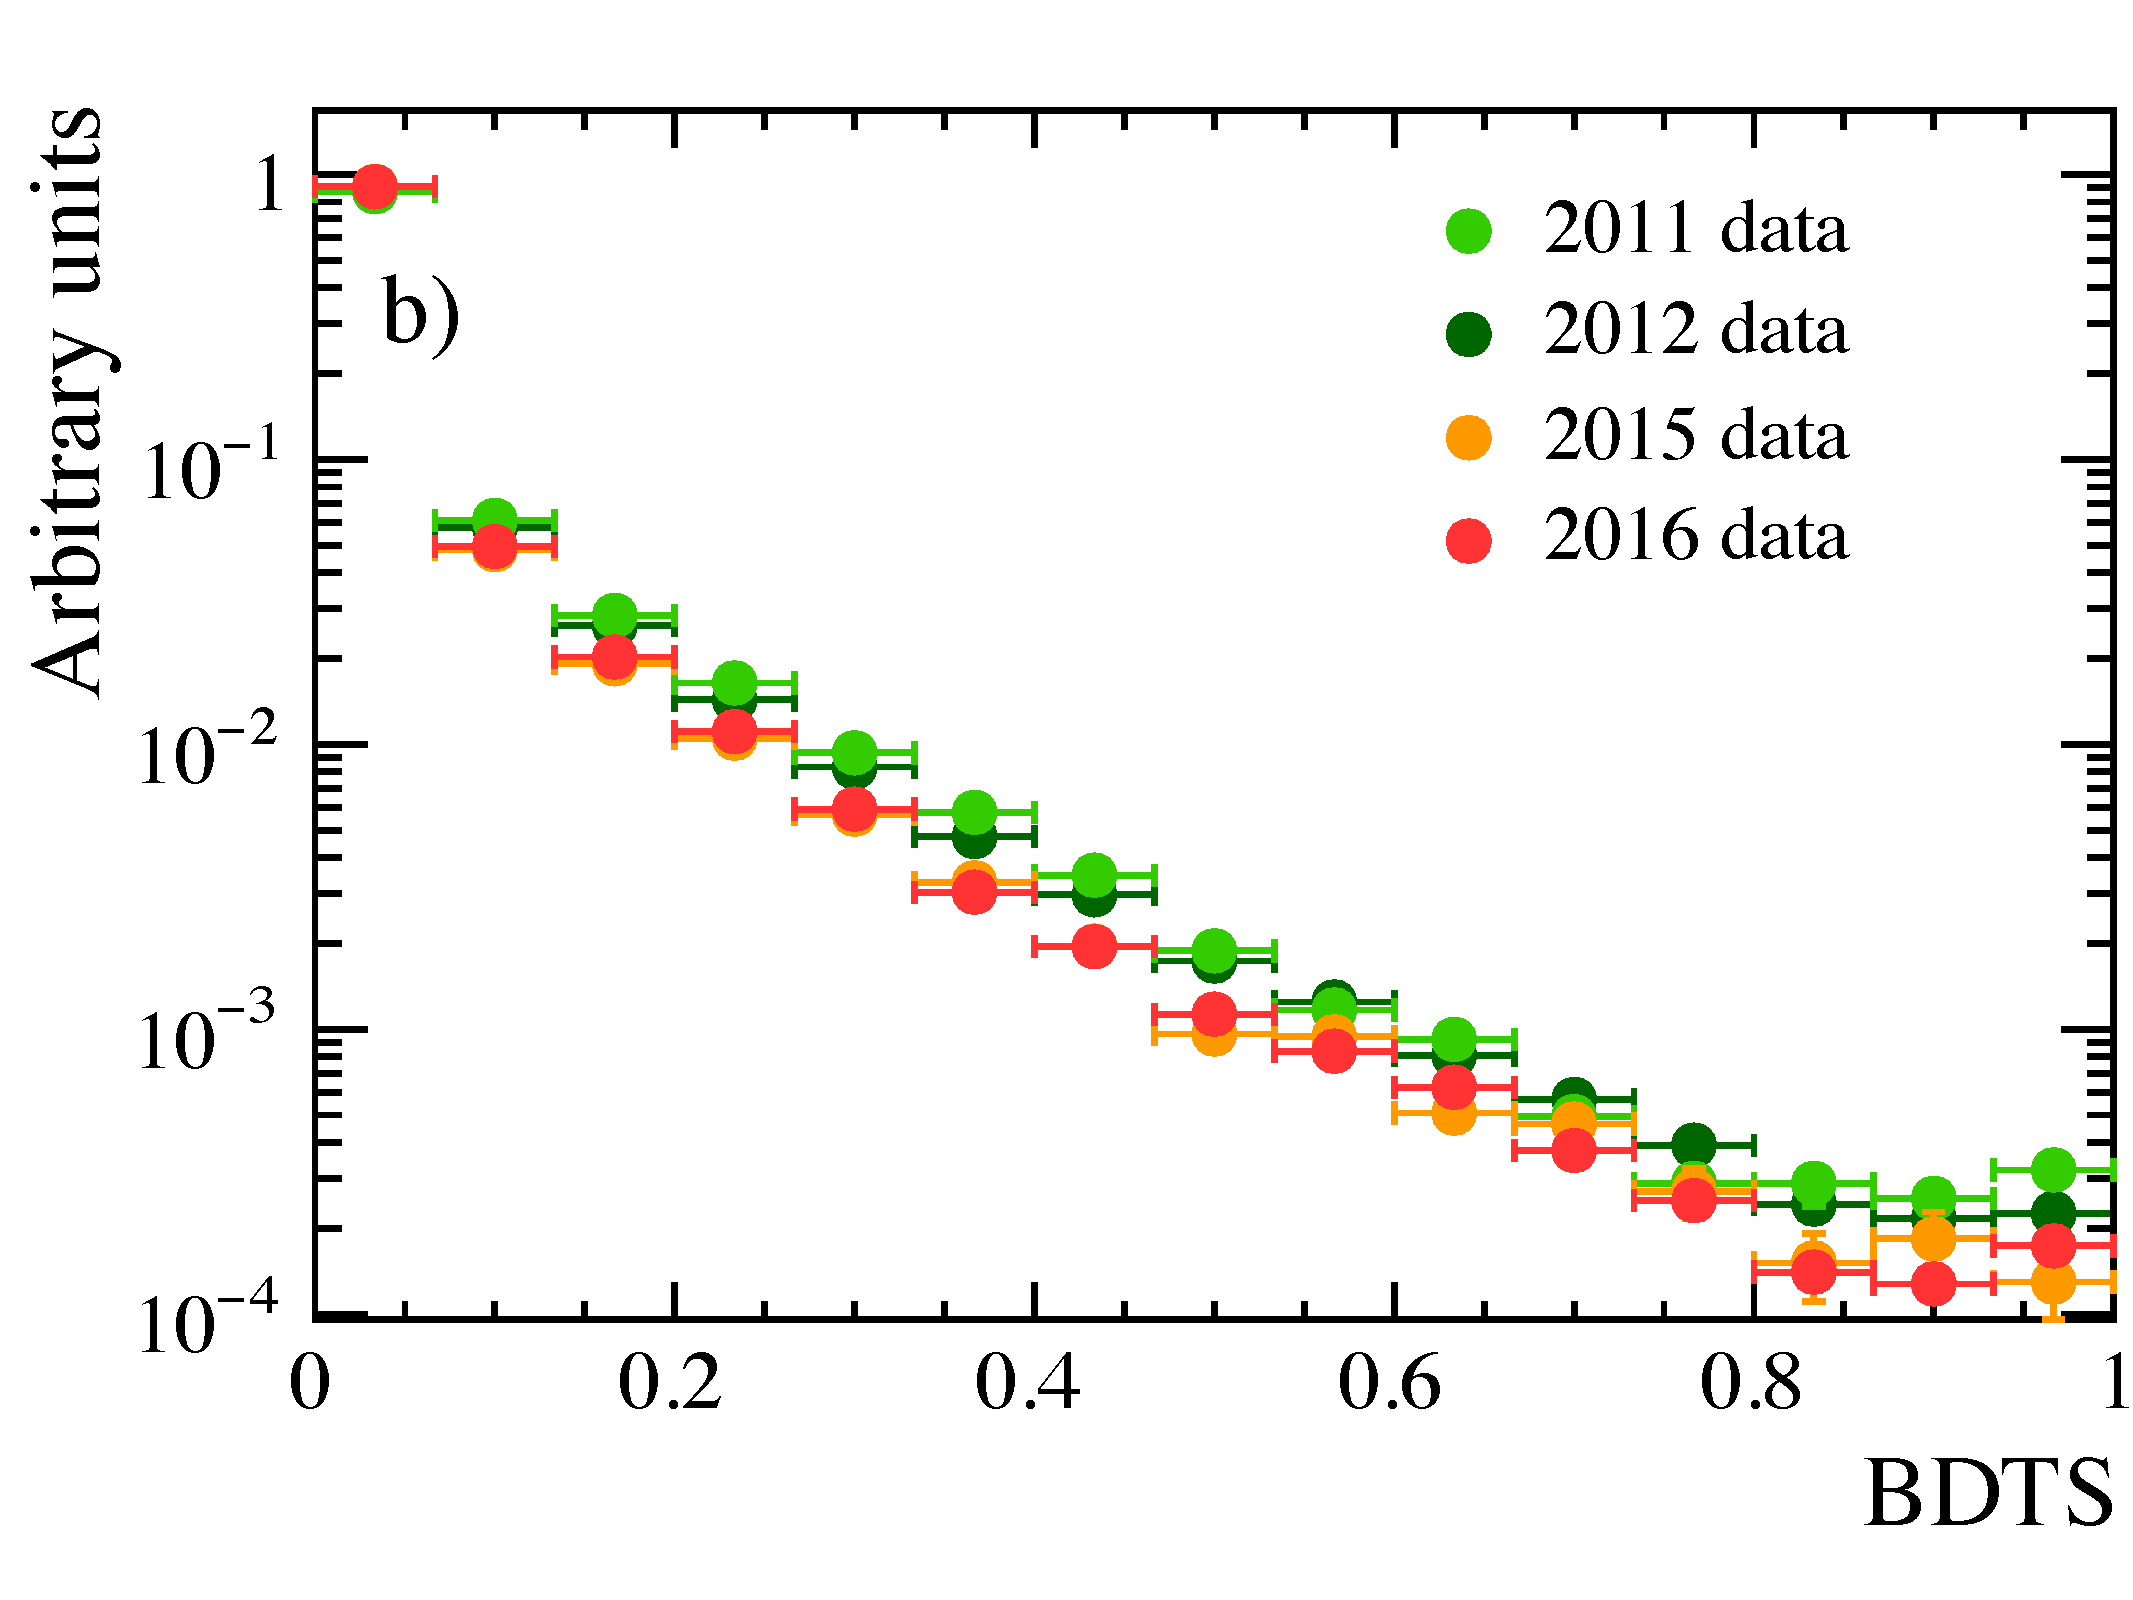
\includegraphics[width=\textwidth]{./Figs/Selection/BDTS_background_Feb6.pdf}
        %\caption{ }
        %\label{fig:BDTSbkg}
    \end{subfigure}
    \caption{BDTS response for simulated \bsmumu decays (left) and data with a mass above 5447 \mevcc consisting on \bbbarmumux decays.}
    \label{fig:FlatteningBDTS}
\end{figure}

\begin{figure}[htbp]
    \centering
   % \begin{subfigure}[b]{0.4\textwidth}
        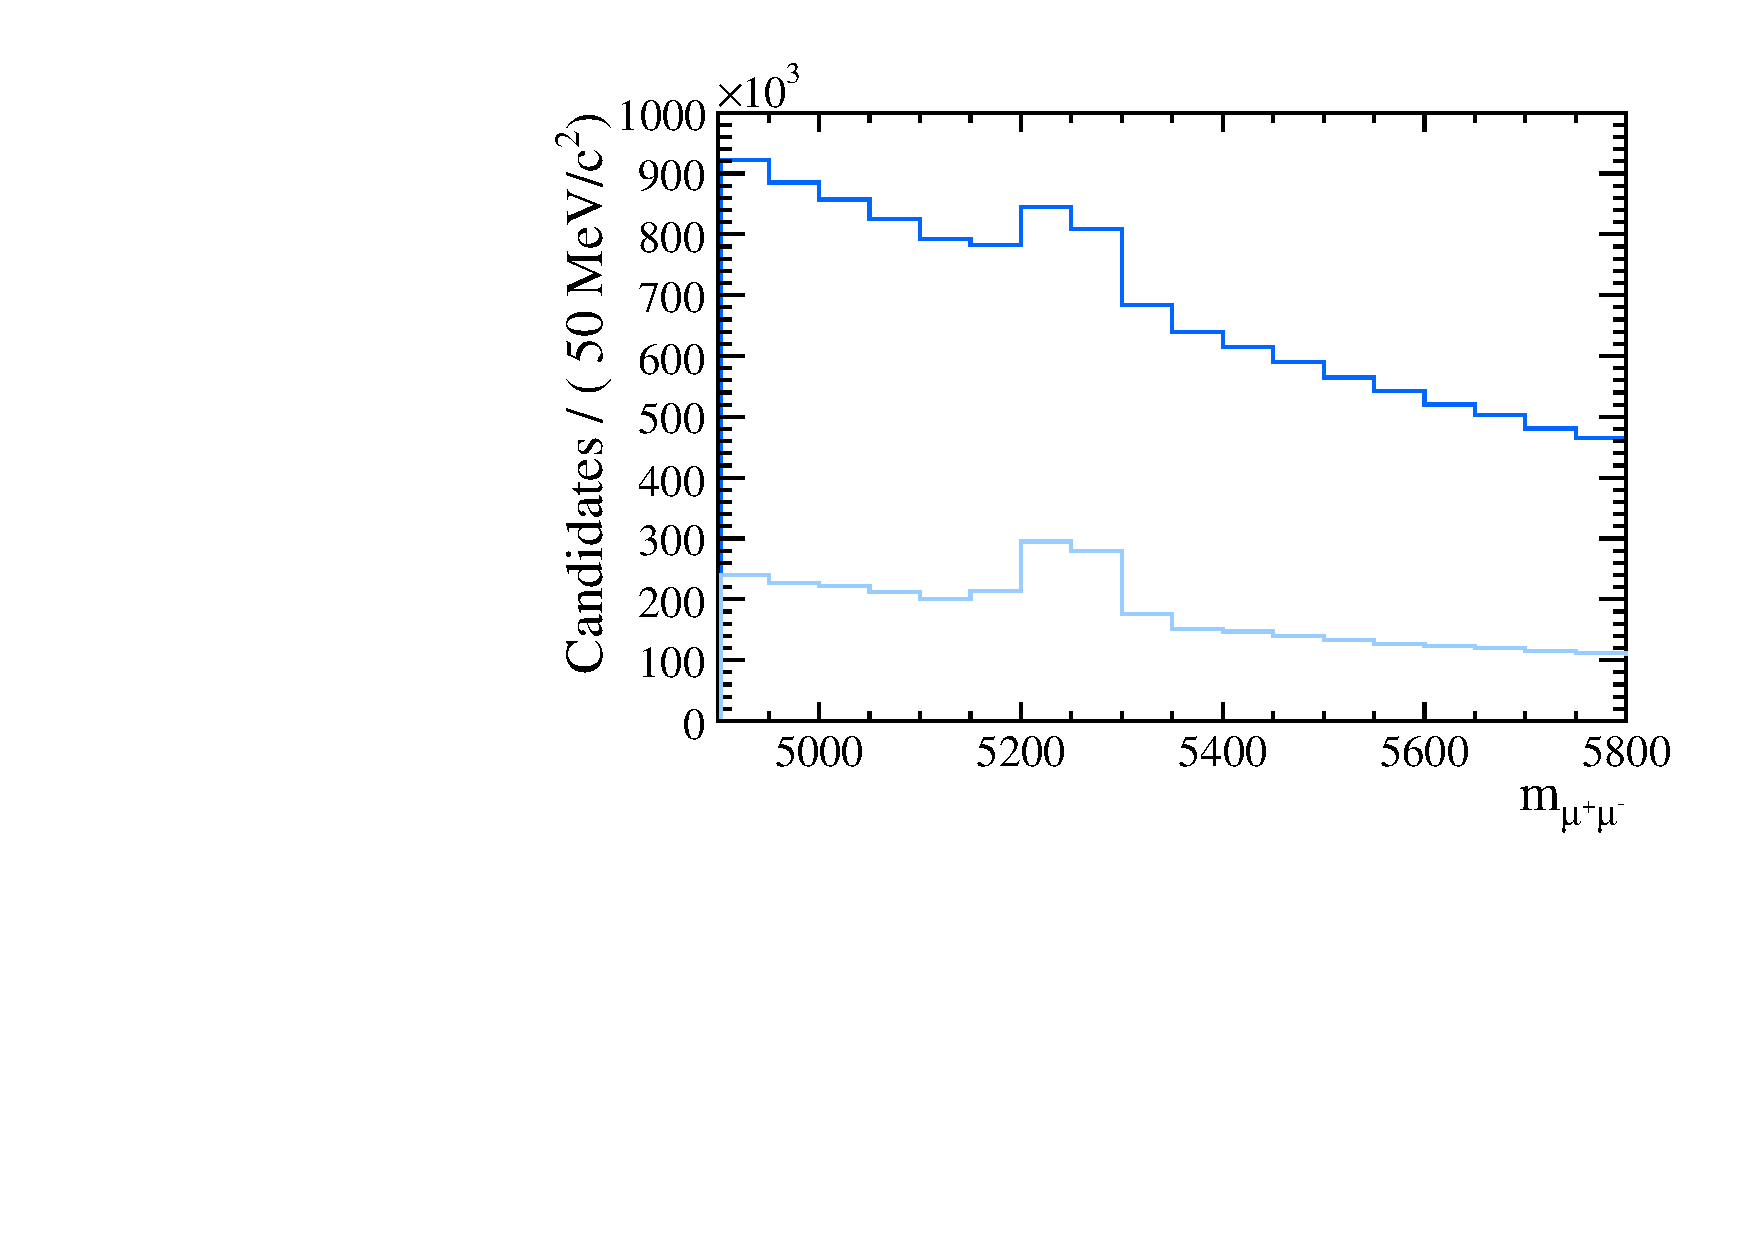
\includegraphics[width= 0.6 \textwidth]{./Figs/Selection/2016_BDTS_impact.pdf}
        %\caption{ }
       % \label{fig:BDTSsig}
    %\end{subfigure}
   % ~ %add desired spacing between images, e. g. ~, \quad, \qquad, \hfill etc. 
      %(or a blank line to force the subfigure onto a new line)
   % \begin{subfigure}[b]{0.4\textwidth}
      % 
\includegraphics[width=\textwidth]{./Figs/placeholder.jpeg}
      %  \caption{ }
     %   \label{fig:BDTSbkg}
  %  \end{subfigure}
    \caption{Invariant mass spectrum for \bhh decays in 2016 data passing the selection requirements in Table~\ref{tab:BDTSpresel} before and after the BDTS cut is applied.}
    \label{fig:BDTSpreformance}
\end{figure}

\begin{table}[htbp]
\begin{center}
\begin{tabular}{ll}
\hline
\multicolumn{2}{c}{Selection applied to BDTS training samples.} \\ \hline
\bs & $\mu^{\pm}$\\
 FD $\chi^{2}$ $>$ 225 & $p_{T}$ $>$ 500 \mevc \\
 IP $\chi^{2}$ $<$ 25  &  track $\chi^{2}$/ndof $<$ 3    \\
 Vertex $\chi^{2}$/ndof $<$ 9    & minimum IP $\chi^{2}$ $>$ 25   \\
 DOCA $<$ 0.3 mm    & 0.25 \gevc $<$ $p_{T}$ $<$ 40 \gevc  \\
 $\tau$ $<$ 13.248 \ps  &  $p$ $<$ 500 \gevc  \\
 $p_{T}$ $>$ 500 \mevc  &  \\ 
DIRA $>$ 0 & \\
\hline
\multicolumn{2}{c}{Trigger requirements} \\ \hline
L0Global&DEC\\
Hlt1Phys&DEC \\
Hlt2Phys&DEC \\ 
\hline
\end{tabular}
\vspace{0.7cm}
\caption{Selection cuts applied to select candidates for signal and background samples used to train the BDTS. The isMuon requirement is not applied to the muons to that the BDTS can be used on \bhh decays. The trigger requirement used are the same as those used in the \bmumu Branching Fraction analysis.}
\label{tab:BDTSpresel}
\end{center}
\vspace{-1.0cm}                                                                                          
\end{table}

\begin{table}[htbp]
\begin{center}
\begin{tabular}{ll}
\hline
Parameter & Value \\ \hline
nTrees & 250 \\
nEventsMin & 400 \\
MaxDepth & 3 \\
%NNodesMax = 100000 \\
$\beta$ & 1.0 \\
nCuts & 20 \\
\hline
\end{tabular}
\vspace{0.7cm}
\caption{Training parameters used to specify the training of the BDTS.}
\label{tab:BDTStrainingparams}
\end{center}
\vspace{-1.0cm}
\end{table}

\subsubsection{Global BDT}
\label{sec:globalBDT}

The global BDT is the final step in identifying \bmumu decays and it is very effective at separating them from long lived combinatorial background decays. The discriminating power achieved by the global BDT is mostly dependant on isolation variables. Isolation variables, or just isolations, provide a measure of how far away each muon from a \bmumu candidate is from other tracks in the event. The tracks of the muons from a real \bmumu decays will be, in general, far from other tracks in the event because the \bmumu decays tree contains no other tracks apart from the muons. However long lived combinatorial background arises from semi-leptonic decays therefore muon tracks are likely to be close to other tracks that have originated from the same decay tree as the muon. %Various different definitions of isolations have been used across different experiments from D0 and CDF to ATLAS, CMS and LHCb. 
Isolations are very useful in the selection of very rare decays like \smumu because they enable background to be removed whilst keeping a high efficiency for signal decays.

Two isolation variables are used in the global BDT, one compares long tracks in the event to the muons in \bmumu candidates and the other compares VELO tracks in the event to the muons. The definition of the track types can be found in Section~\ref{sec:Trackrecon}. The isolation variables are built from the output of BDTs. For each type of track a BDT is trained on simulated \bsmumu and \bbbarmumux decays using a set of input variables that describe track and vertex properties. The BDT compares the $\mu^{+}$ from a \bsmumu candidate with all other tracks in the event, excluding the track of the $\mu^{-}$, and gives an output, {\it iso$_{\mu^{+}}$(track)}, for each possible $\mu^{+}$ and track pairing. The process is repeated for the $\mu^{-}$. The BDT is designed to produce high output values for muons from \bbbarmumux decays and a low value for muons from \bsmumu decays. The isolation variable of a \bsmumu candidate is then composed of the sum of the highest values of {\it iso$_{\mu^{+}}$(track)} and {\it iso$_{\mu^{-}}$(track)} for any tracks in the event. The separation power of these isolations are shown in Figure~\ref{fig:Isolations}. %Full details of the isolation development can be found in~\ref{}.

\begin{figure}[htbp]
    \centering
        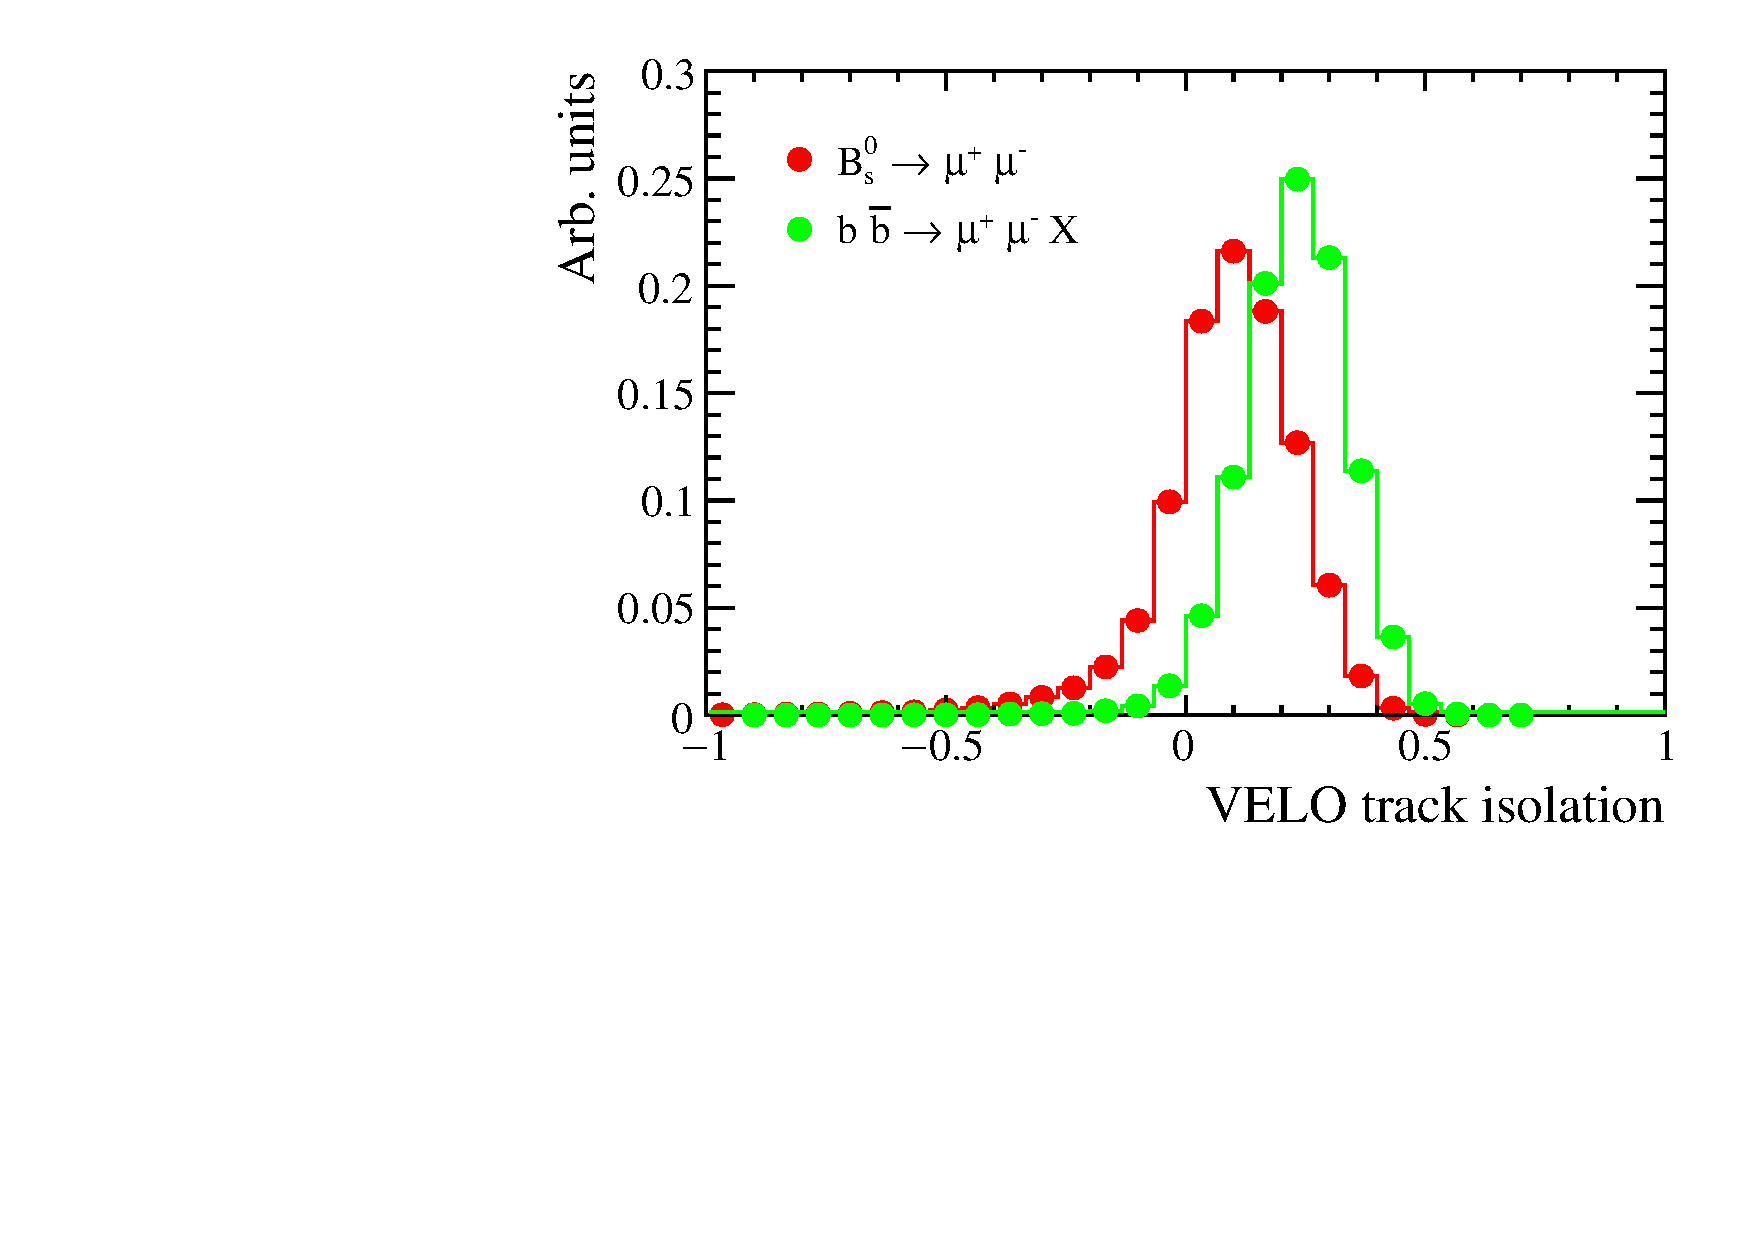
\includegraphics[width=0.49\textwidth]{./Figs/Selection/iso_velo_simulation_all.pdf}
              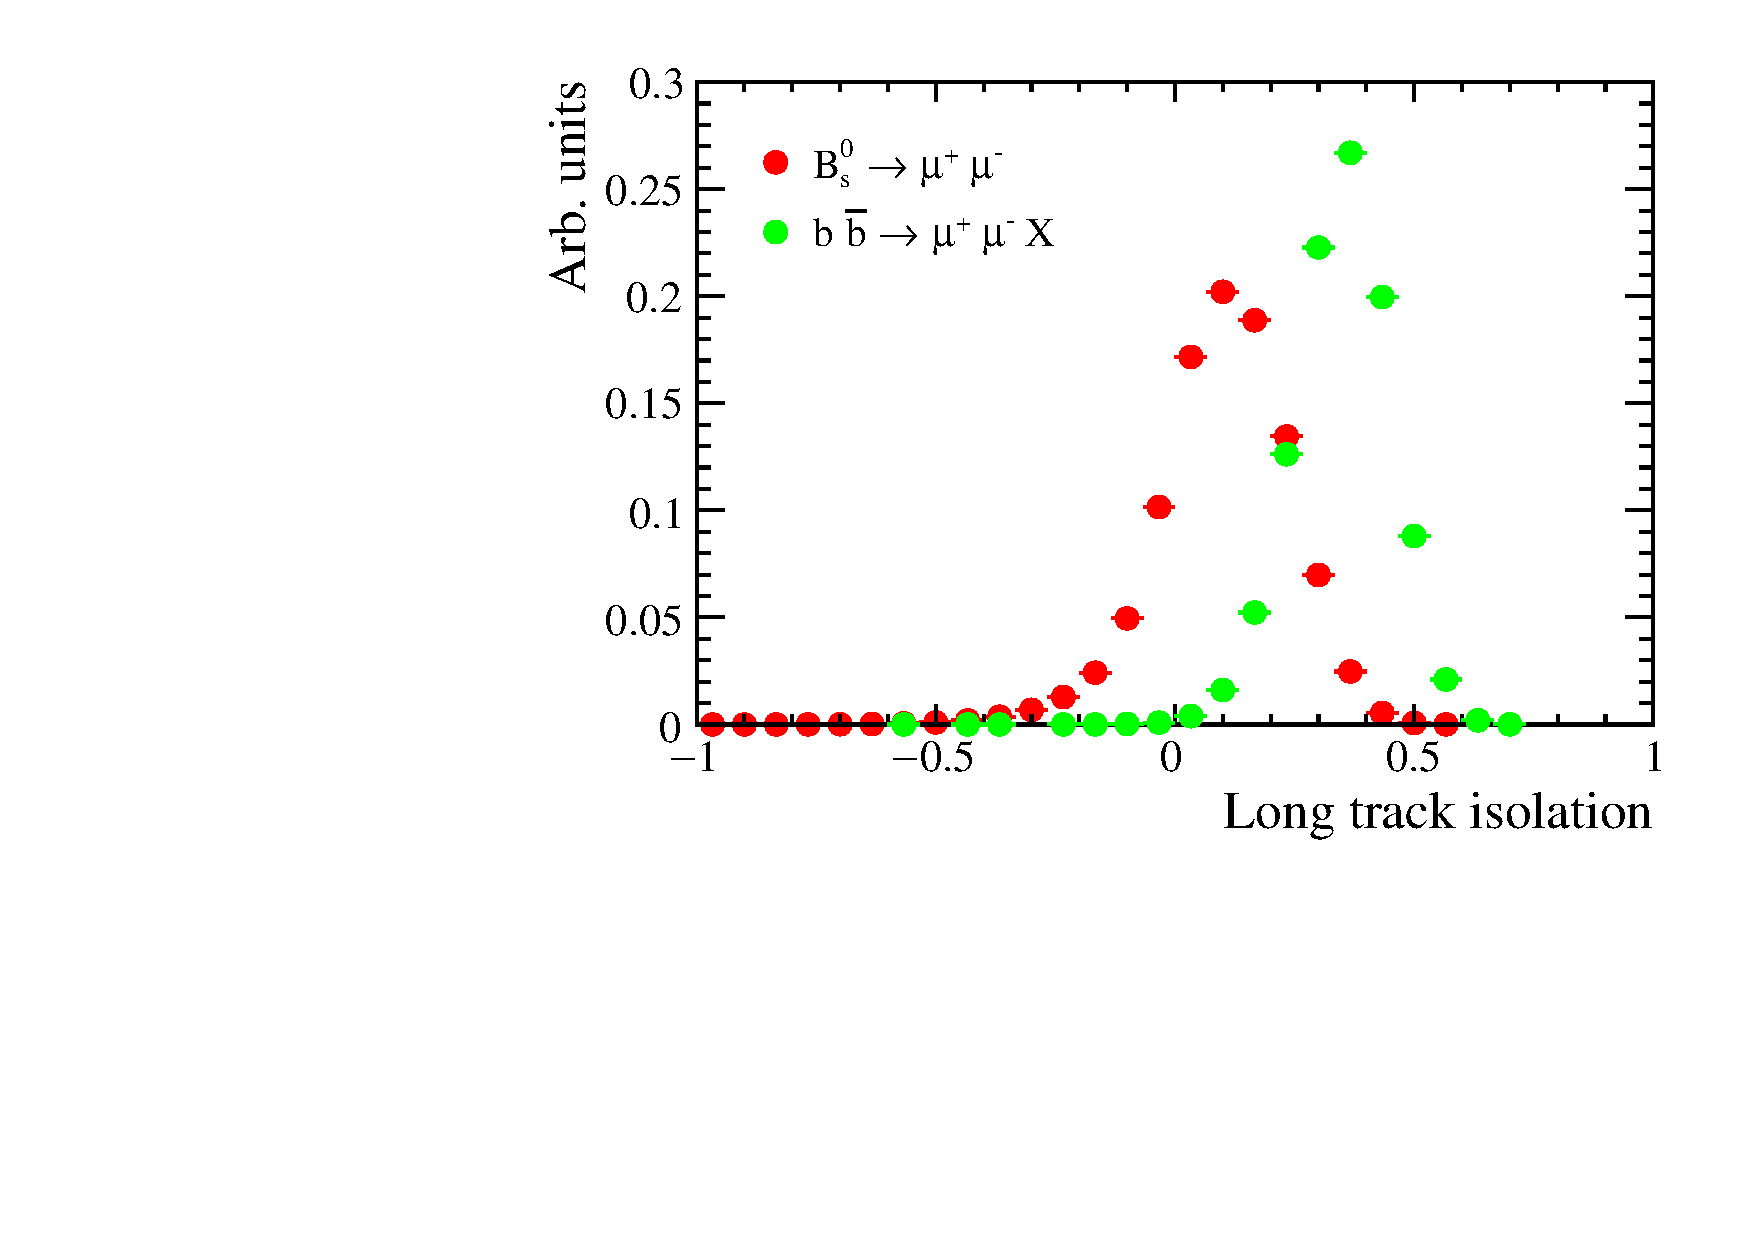
\includegraphics[width=0.49\textwidth]{./Figs/Selection/iso_lt_sim_all.pdf}
           \caption{Long track and VELO track isolation distributions of simulated \bsmumu and \bbbarmumux decays used to train the global BDT passing cuts in Table~\ref{tab:BDTpresel}.}
    \label{fig:Isolations}
\end{figure}

The isolations are used along with five other variables in the global BDT. The full list of input variables used are;
\begin{itemize}
\item Long track isolation
\item VELO track isolation
\item $\sqrt{\Delta \phi^{2} + \Delta \eta^{2}}$, where $\Delta \phi$ is the difference in azimuthal angles of the muons and $\Delta \eta$ the difference in the pseudorapidity of the muons
\item the smallest IP \chisqd with respect to the primary vertex of the \bsmumu of the muons
\item vertex \chisqd of the \bs
\item IP \chisqd of the \bs with respect to the primary vertex
\item angle between the momentum vector of the \bs and the vector connecting the production and decay vertices of the \bs
\end{itemize}

A comparison of the signal and background distributions of the input variables are shown in Figures~\ref{fig:Isolations} and \ref{fig:BDTvars}. These variables were chosen by training a BDT beginning with the most discriminating variable, the Long track isolation, and adding variables to determine which improved the performance to the classifier. Only variables that improved the performance were included in the global BDT. The training parameters used in the BDT are listed in Table~\ref{tab:BDTtrainingparams}. These parameters were chosen by scanning across a range of variables and choosing those that gave the best performance. 

\begin{figure}[htbp]
    \centering
        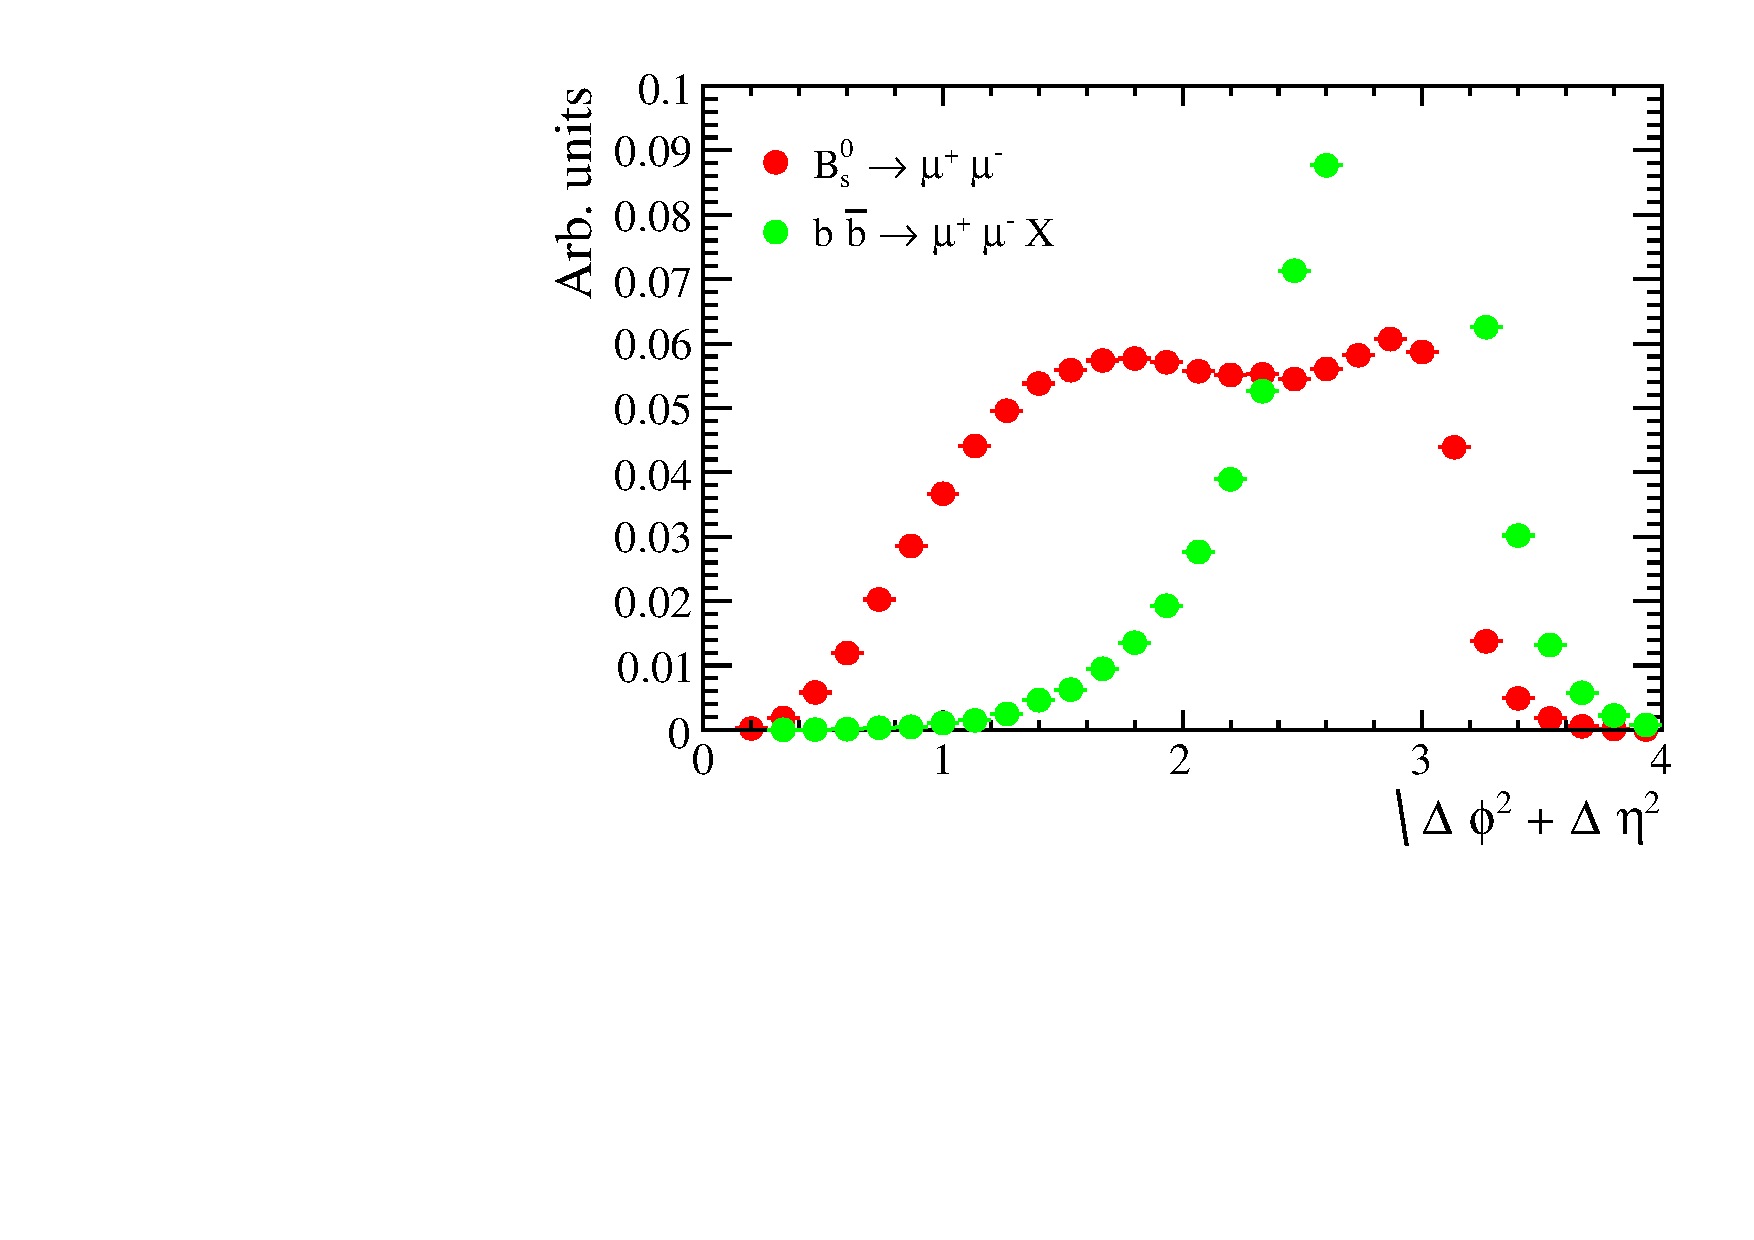
\includegraphics[width=0.49\textwidth]{./Figs/Selection/var1_sim_all.pdf}
       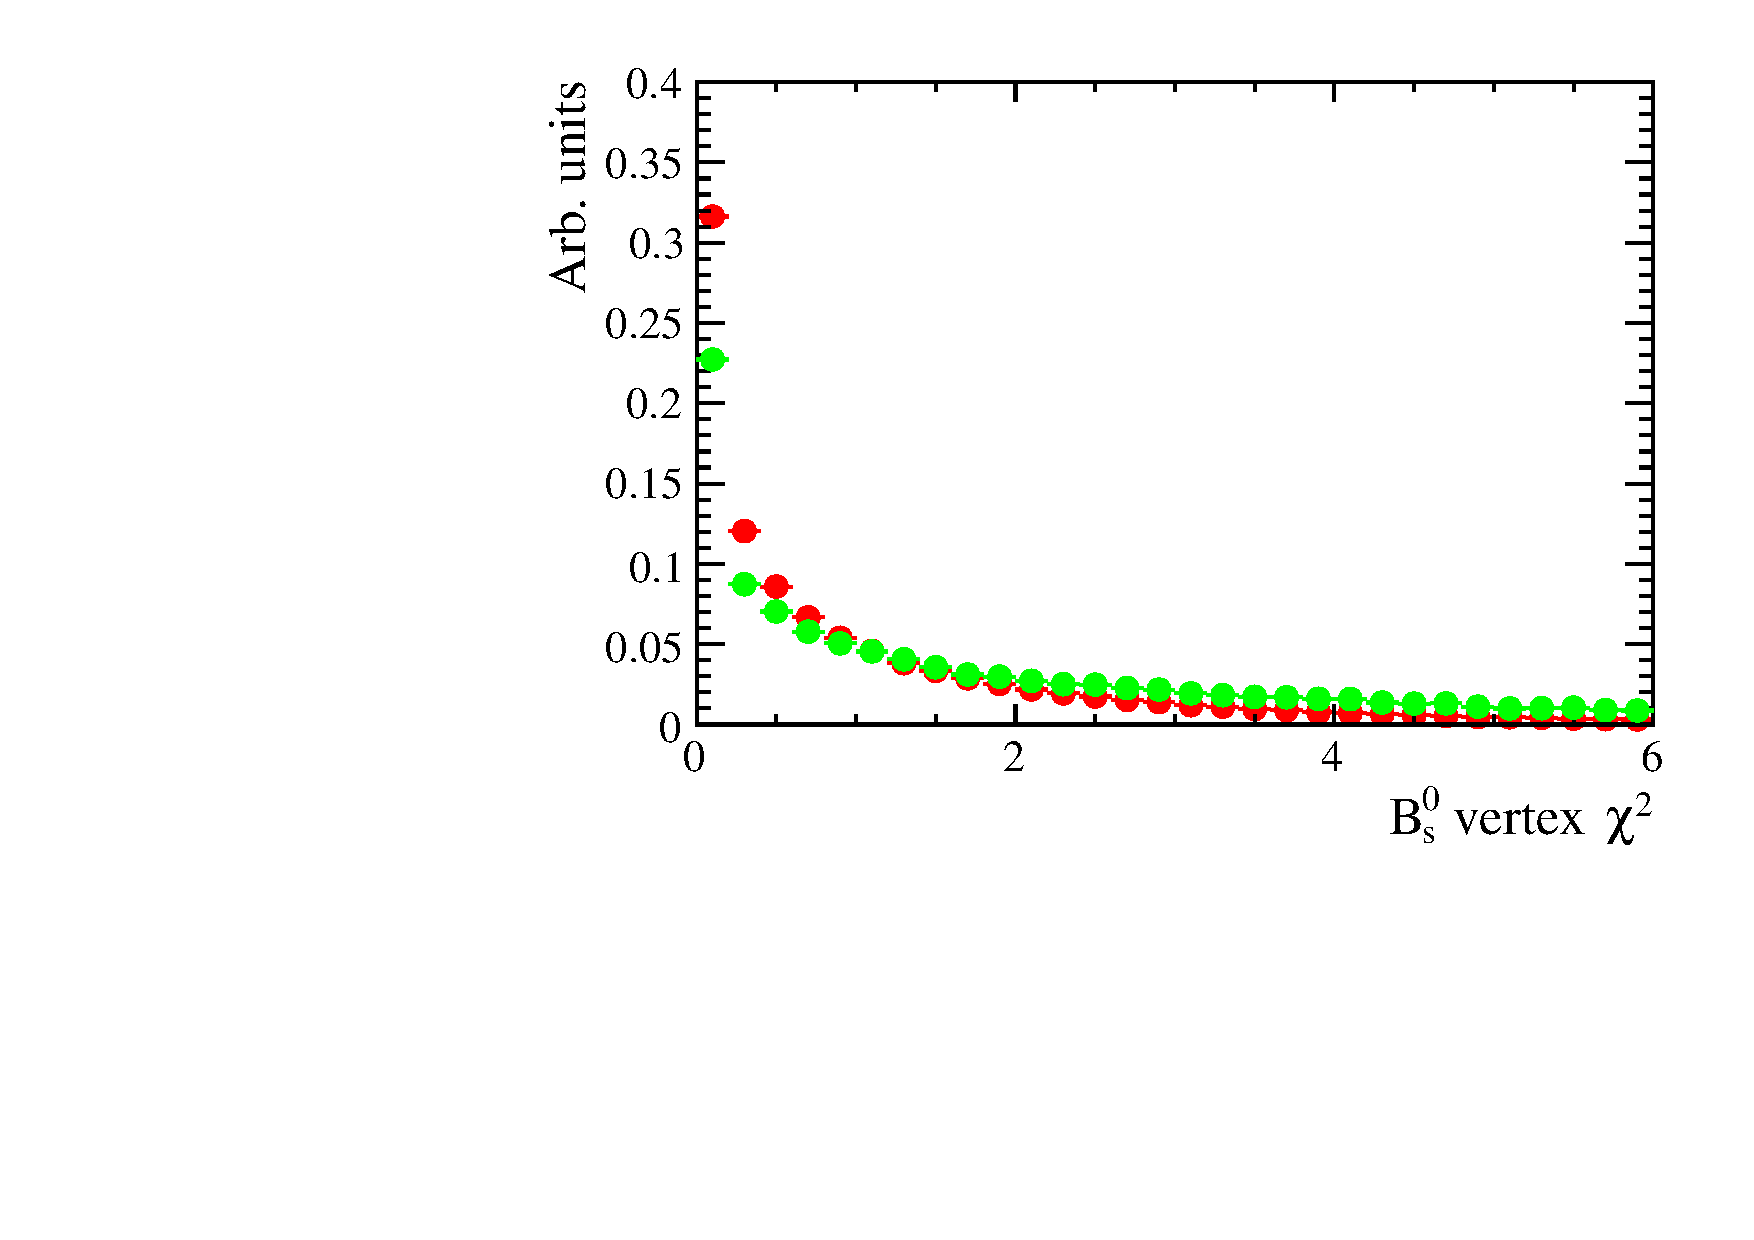
\includegraphics[width=0.49\textwidth]{./Figs/Selection/var2_sim_all.pdf}
 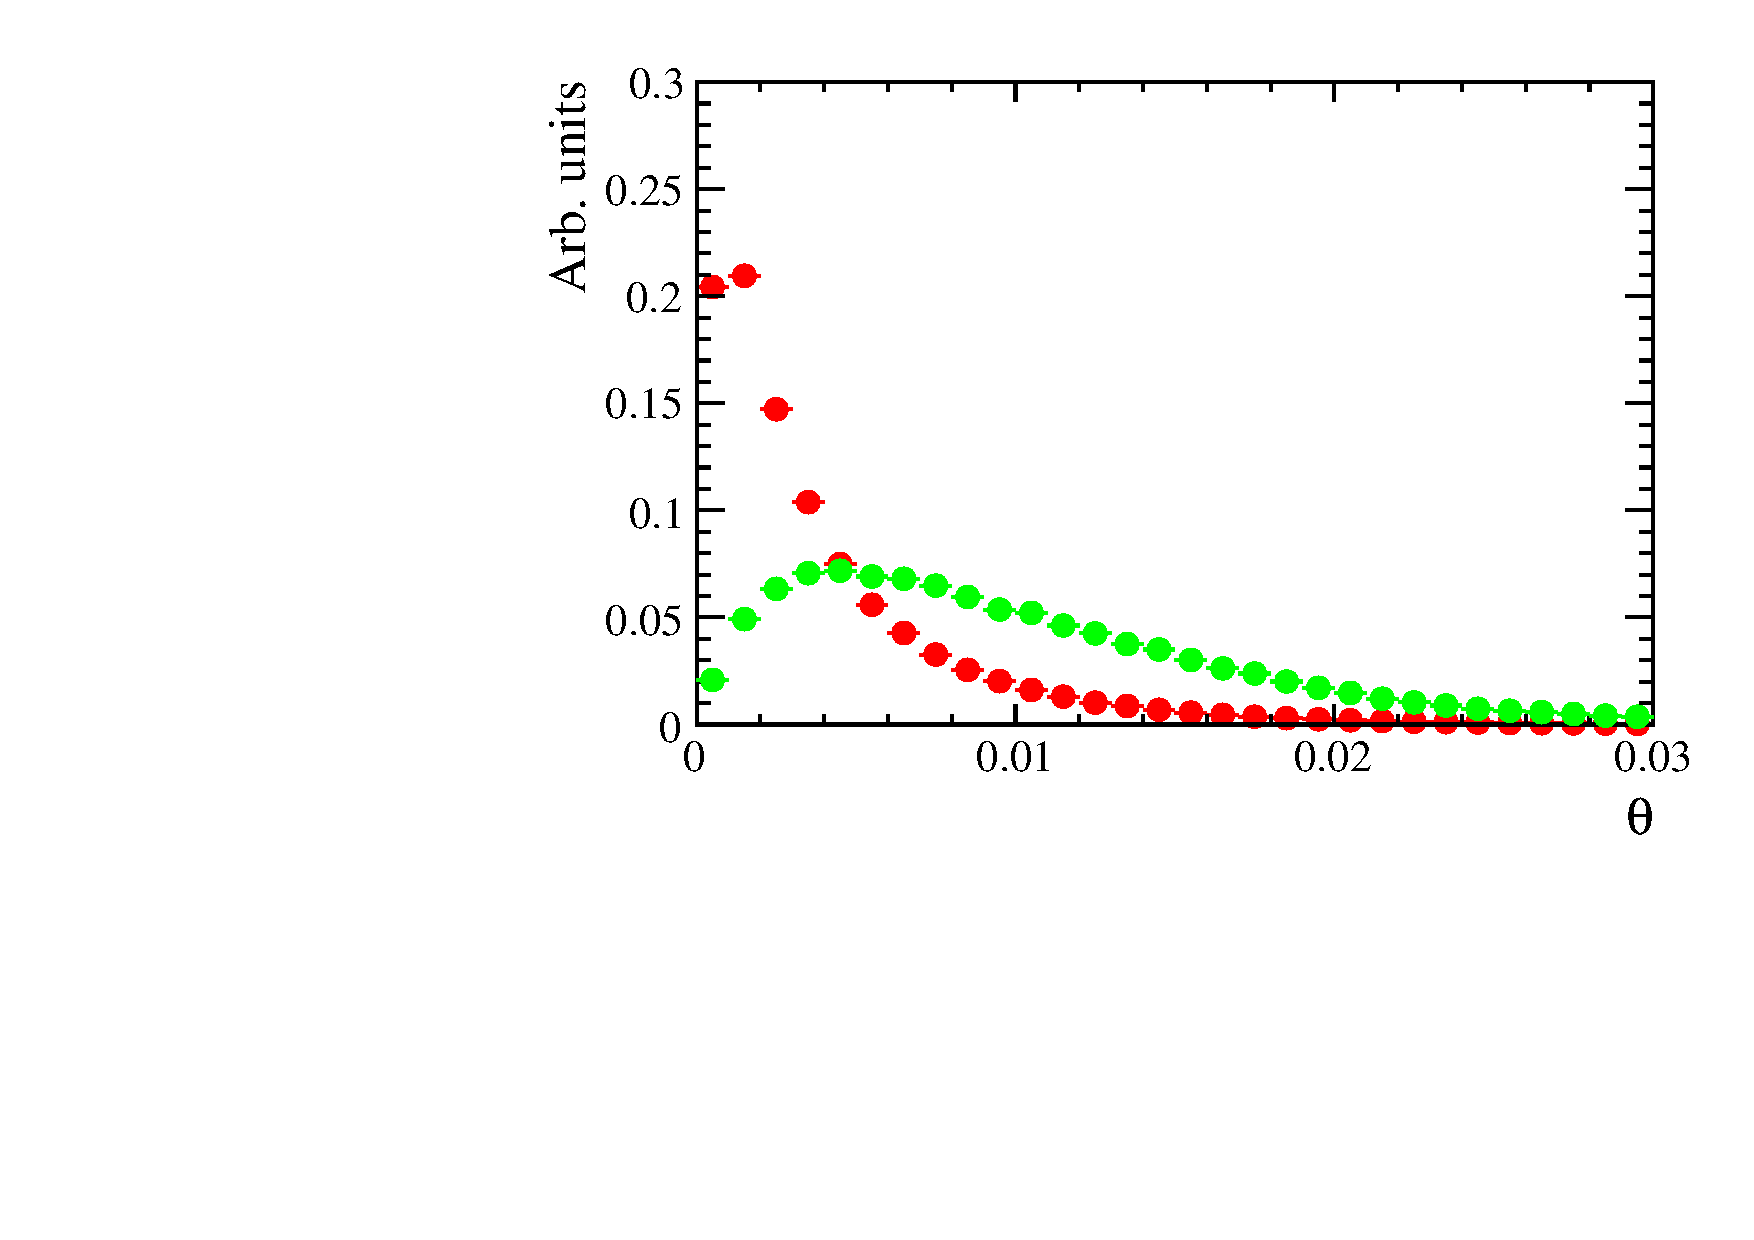
\includegraphics[width=0.49\textwidth]{./Figs/Selection/var3_sim_all.pdf}
 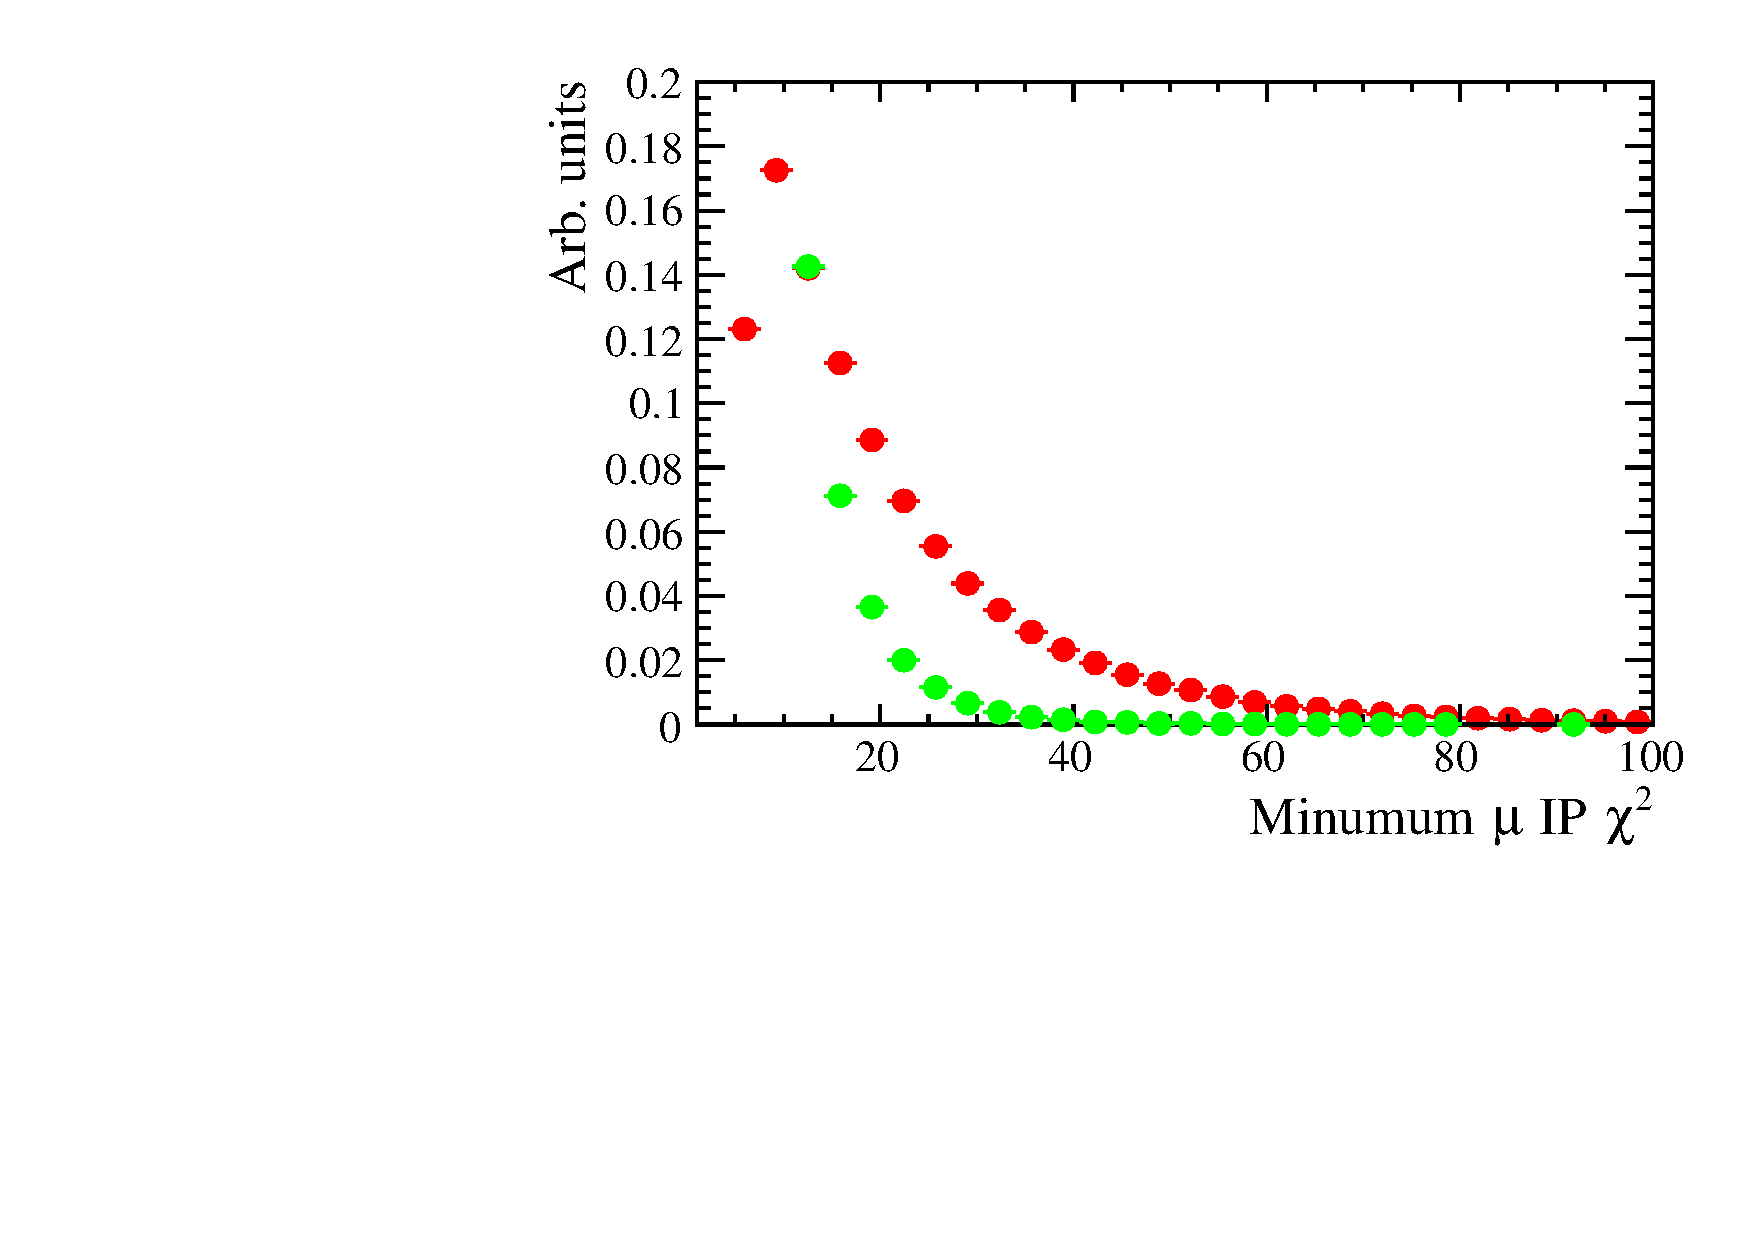
\includegraphics[width=0.49\textwidth]{./Figs/Selection/var4_sim_all.pdf}
 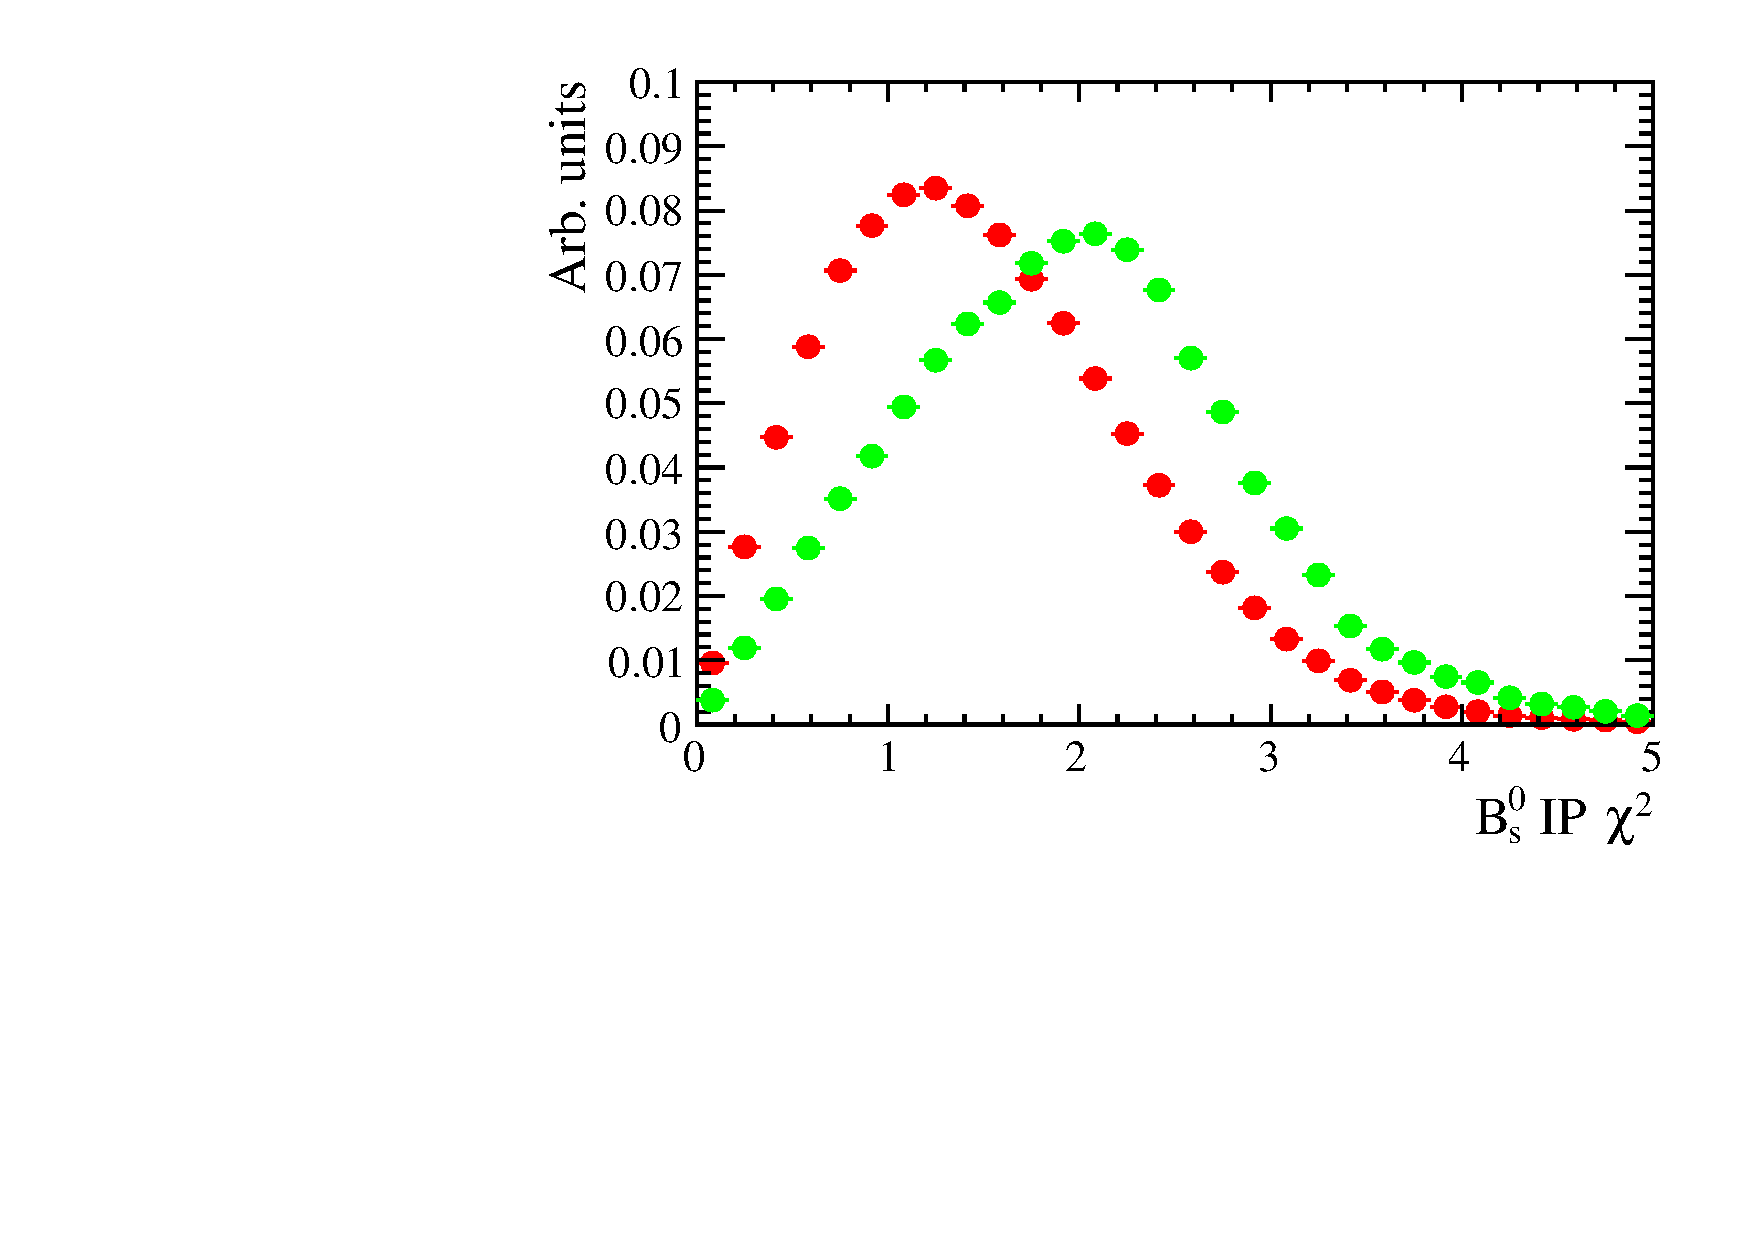
\includegraphics[width=0.49\textwidth]{./Figs/Selection/var5_sim_all.pdf}

    \caption{Distributions of input variables of the global BDT from simulated \bsmumu and \bbbarmumux decays used to train the global BDT passing cuts in Table~\ref{tab:BDTpresel}.}
    \label{fig:BDTvars}
\end{figure}


\begin{table}[htbp]
\begin{center}
\begin{tabular}{ll}
\hline
Parameter & Value \\ \hline
nTrees & 1000 \\
%nEventsMin & 400 \\
MinNodeSize & 1$\%$ \\
MaxDepth & 3 \\
%NNodesMax = 100000 \\
$\beta$ & 0.75 \\
nCuts & 30 \\
\hline
\end{tabular}
\vspace{0.7cm}
\caption{Training parameters used to specify the training of the global BDT.}
\label{tab:BDTtrainingparams}
\end{center}
\vspace{-1.0cm}
\end{table}

 %The global BDT was trained on simulated \bsmumu and \bbbarmumux decays with 2012 data taking conditions for the signal and background samples. The simulated decas had to pass the selection requirements listed in Table~\ref{}. Independant samples were used for training and testing the global BDT. 


Simulated \bsmumu and \bbbarmumux decays are used to provide large signal and background training samples for the global BDT. In data \bsmumu candidates in the mass range 5431 to 6550 \mevcc consist almost entirely of \bbbarmumux decays, however the number of candidates in this mass range is too small to be a useful as sample of background candidates to train a BDT with comparable performance to one trained entirely on simulated decays. 
The simulated sample \bbbarmumux decays corresponds to the background expected with 7~\fb of data from $pp$ collisions at $\sqrt{s}$~=~8~\tev. The production of such a large sample requires a lot of space to be saved, therefore several measures were taken to reduce the size needed to save the simulated \bbbarmumux decays. The cuts, listed in Table~\ref{tab:MC_decays}, were applied to the simulated decays as they were generated to reduce the number of events saved on disk. Also the stripping selection cuts in Table~\ref{tab:PreviousStripping} were applied and candidates that did not pass the stripping selection were not saved. Unfortunately the \bbbarmumux sample therefore does not include candidates that are selected by the looser stripping selection described in Section~\ref{}. In order to gain the best BDT performance on data the same cuts should be applied to data that are applied to the samples used to train the BDT. Therefore the original cuts on FD \chisqd and daughter IP \chisqd listed in Table~\ref{tab:PreviousStripping} must be used to select \bsmumu candidates. 
The complete list of selection requirements applied to the training samples used to develop global BDT are listed in Table~\ref{tab:BDTpresel}, the same selection is applied to \bsmumu and \bbbarmumux decays.  
\begin{table}[htbp]
\begin{center}

\begin{tabular}{ll}
\hline
\multicolumn{2}{c}{Selection applied to BDTS training samples.} \\ \hline
\bs & $\mu^{\pm}$\\
 FD $\chi^{2}$ $>$ 225 & $p_{T}$ $>$ 500 \mevc \\
 IP $\chi^{2}$ $<$ 25  &  track $\chi^{2}$/ndof $<$ 3    \\
 Vertex $\chi^{2}$/ndof $<$ 9    & minimum IP $\chi^{2}$ $>$ 25   \\
 DOCA $<$ 0.3 mm    & 0.25 \gevc $<$ $p_{T}$ $<$ 40 \gevc  \\
 $\tau$ $<$ 13.248 \ps  &  $p$ $<$ 500 \gevc  \\
 $p_{T}$ $>$ 500 \mevc  &  isMuon = True\\ 
DIRA $>$ 0 & BDTS > 0.05 \\
4900 $<$ M$_{\mu^{+}\mu^{-}}$ < 6000 \mevcc & \\
\hline
\multicolumn{2}{c}{Trigger requirements} \\ \hline
L0Global&DEC\\
Hlt1Phys&DEC \\
Hlt2Phys&DEC \\ 
\hline
\end{tabular}
\vspace{0.7cm}
\caption{Selection cuts applied to select candidates for signal and background samples used to train the BDT. The trigger requirements imposed are those used to select decays for the \bmumu Branching Fraction measurement.}
\label{tab:BDTpresel}
\end{center}
\vspace{-1.0cm}
\end{table}

The global BDT is used for data taken in all years and in the same way as the BDTS the final output of the global BDT is flattened to have a response between 0 and 1 that is uniform for signal and the background peaks at zero, as shown in Figure~\ref{fig:FlatteningBDT} for each year of data taking. The flattening is important for the measurement of the \bmumu branching fractions because a simultaneous fit is applied to the dimuon invariant mass in bins of BDT, flattening the BDT output enable bins containing equal proportions of signal decays to be easily created. The signal efficiency and background rejection of the global BDT is shown in Figure~\ref{fig:BDTperformance} for all years of data taking, the performance is similar across all the years but with Run 2 data having a slightly better background rejection for a given signal efficiency. 


\begin{figure}[htbp]
    \centering
    \begin{subfigure}[b]{0.48\textwidth}
        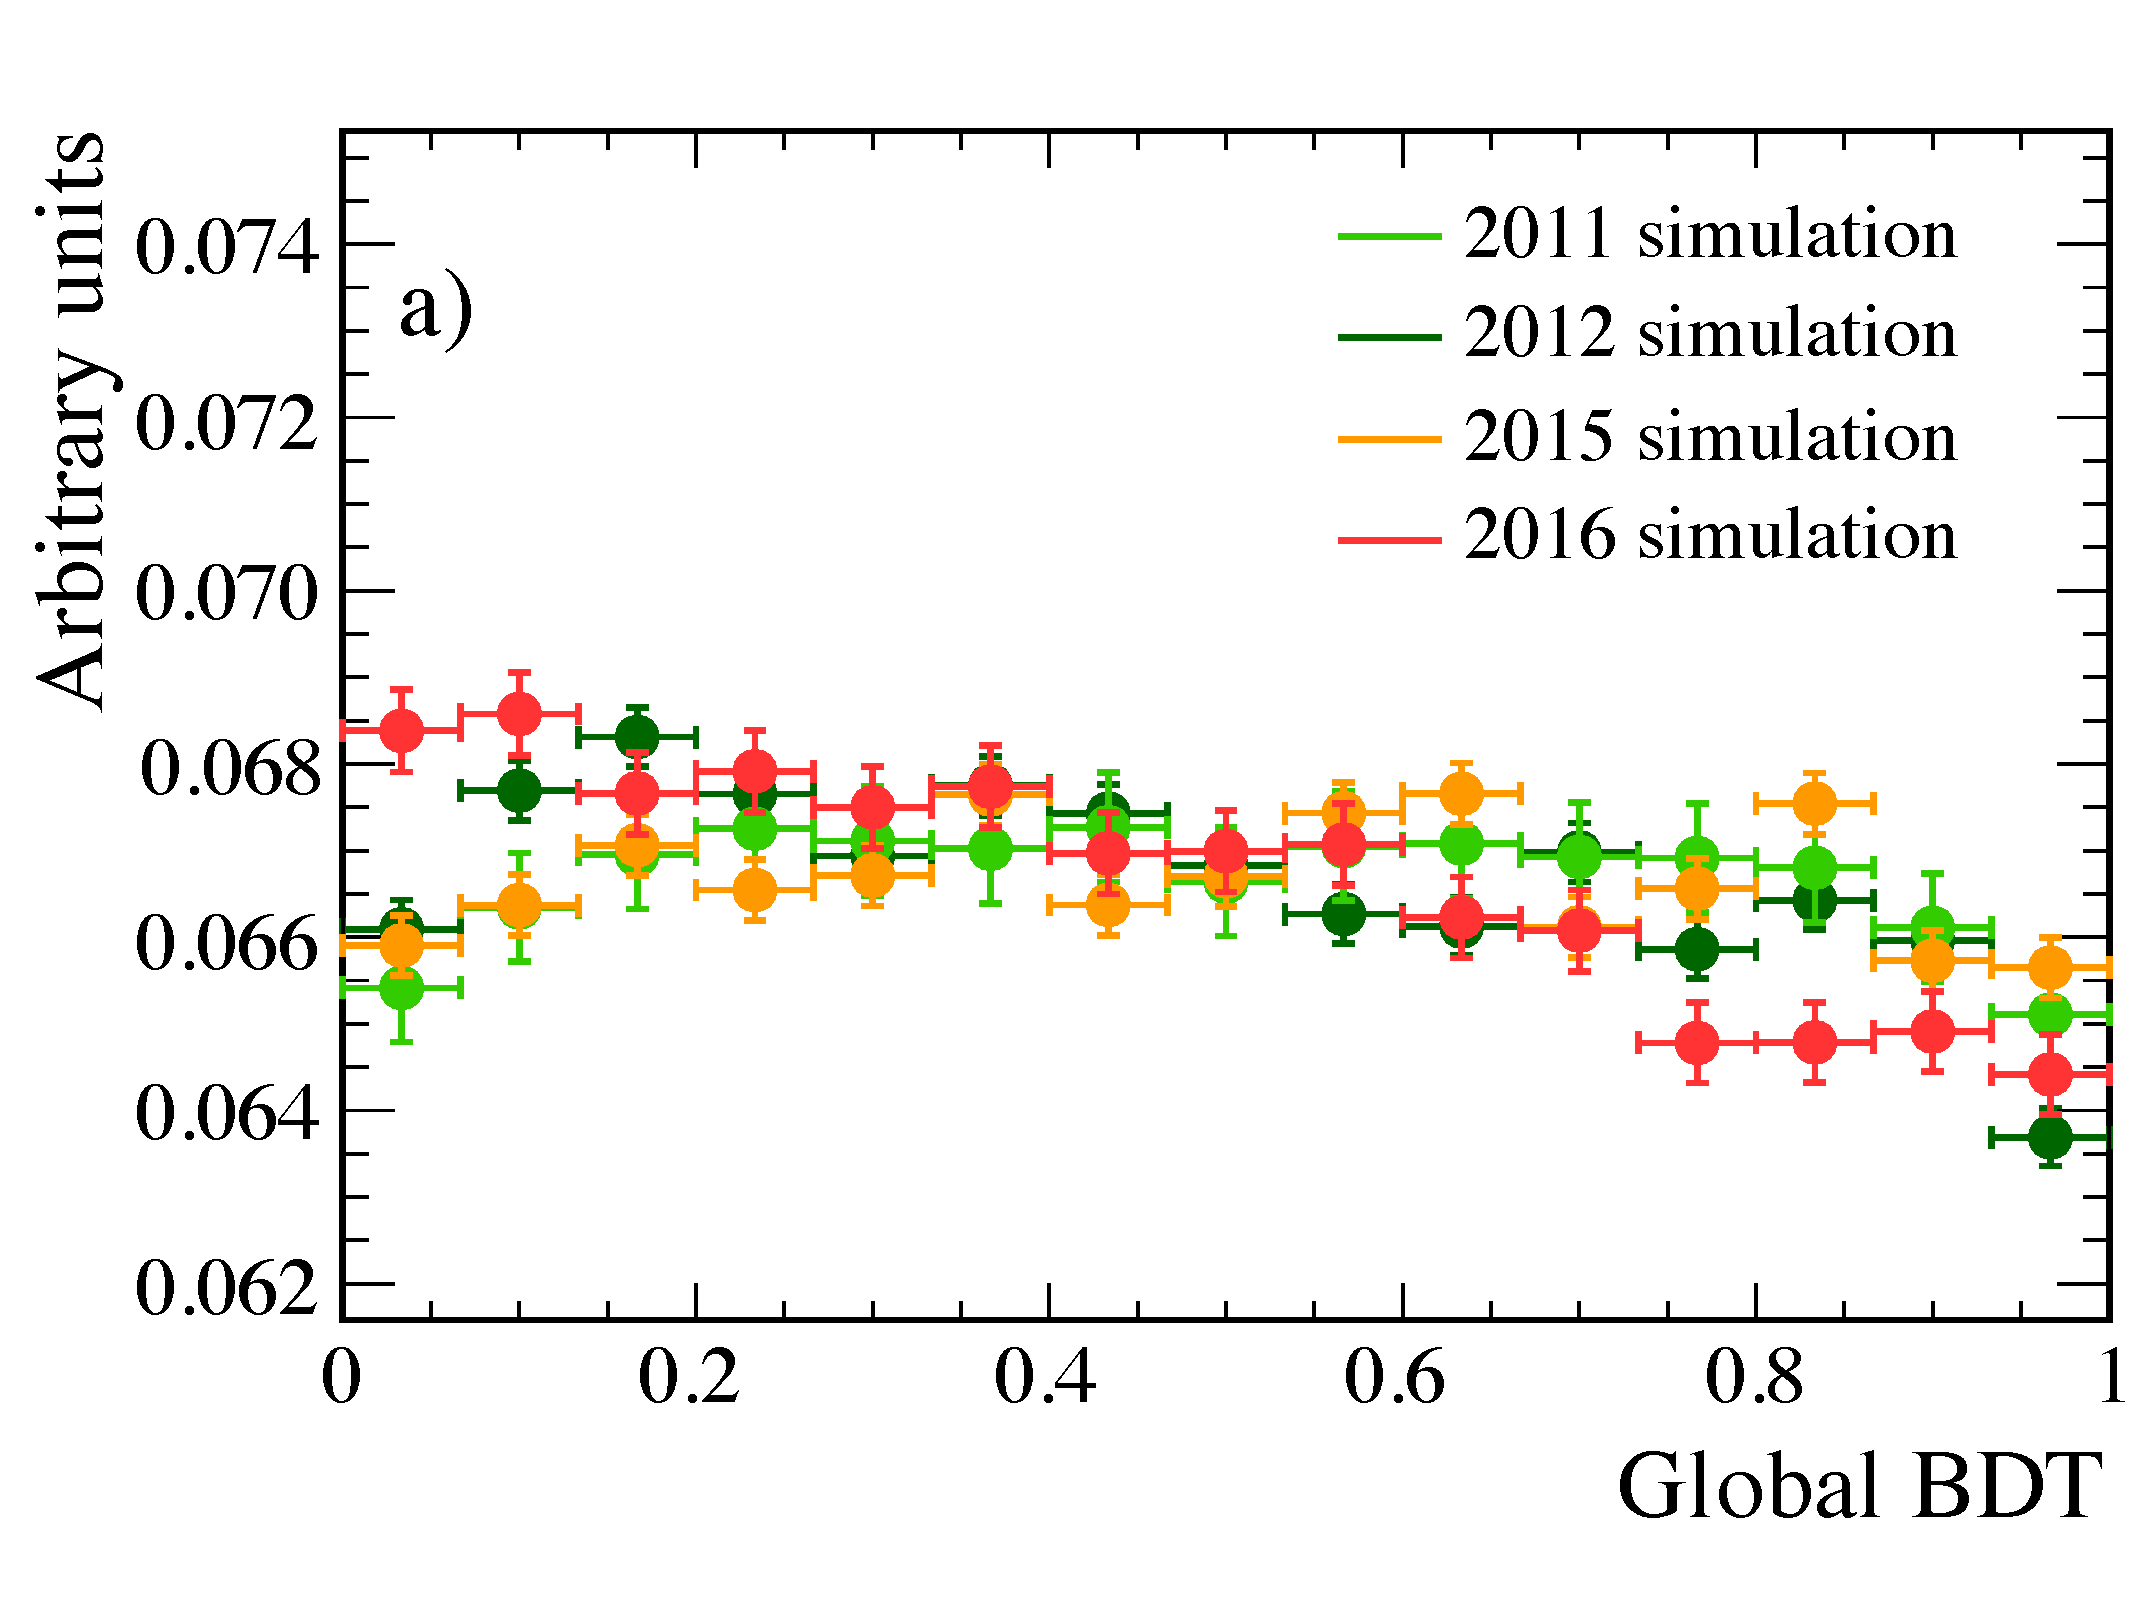
\includegraphics[width=\textwidth]{./Figs/Selection/BDTflat_signal.pdf}
        %\caption{ }
        %\label{fig:BDTsig}
    \end{subfigure}
    ~ %add desired spacing between images, e. g. ~, \quad, \qquad, \hfill etc. 
      %(or a blank line to force the subfigure onto a new line)
    \begin{subfigure}[b]{0.48\textwidth}
       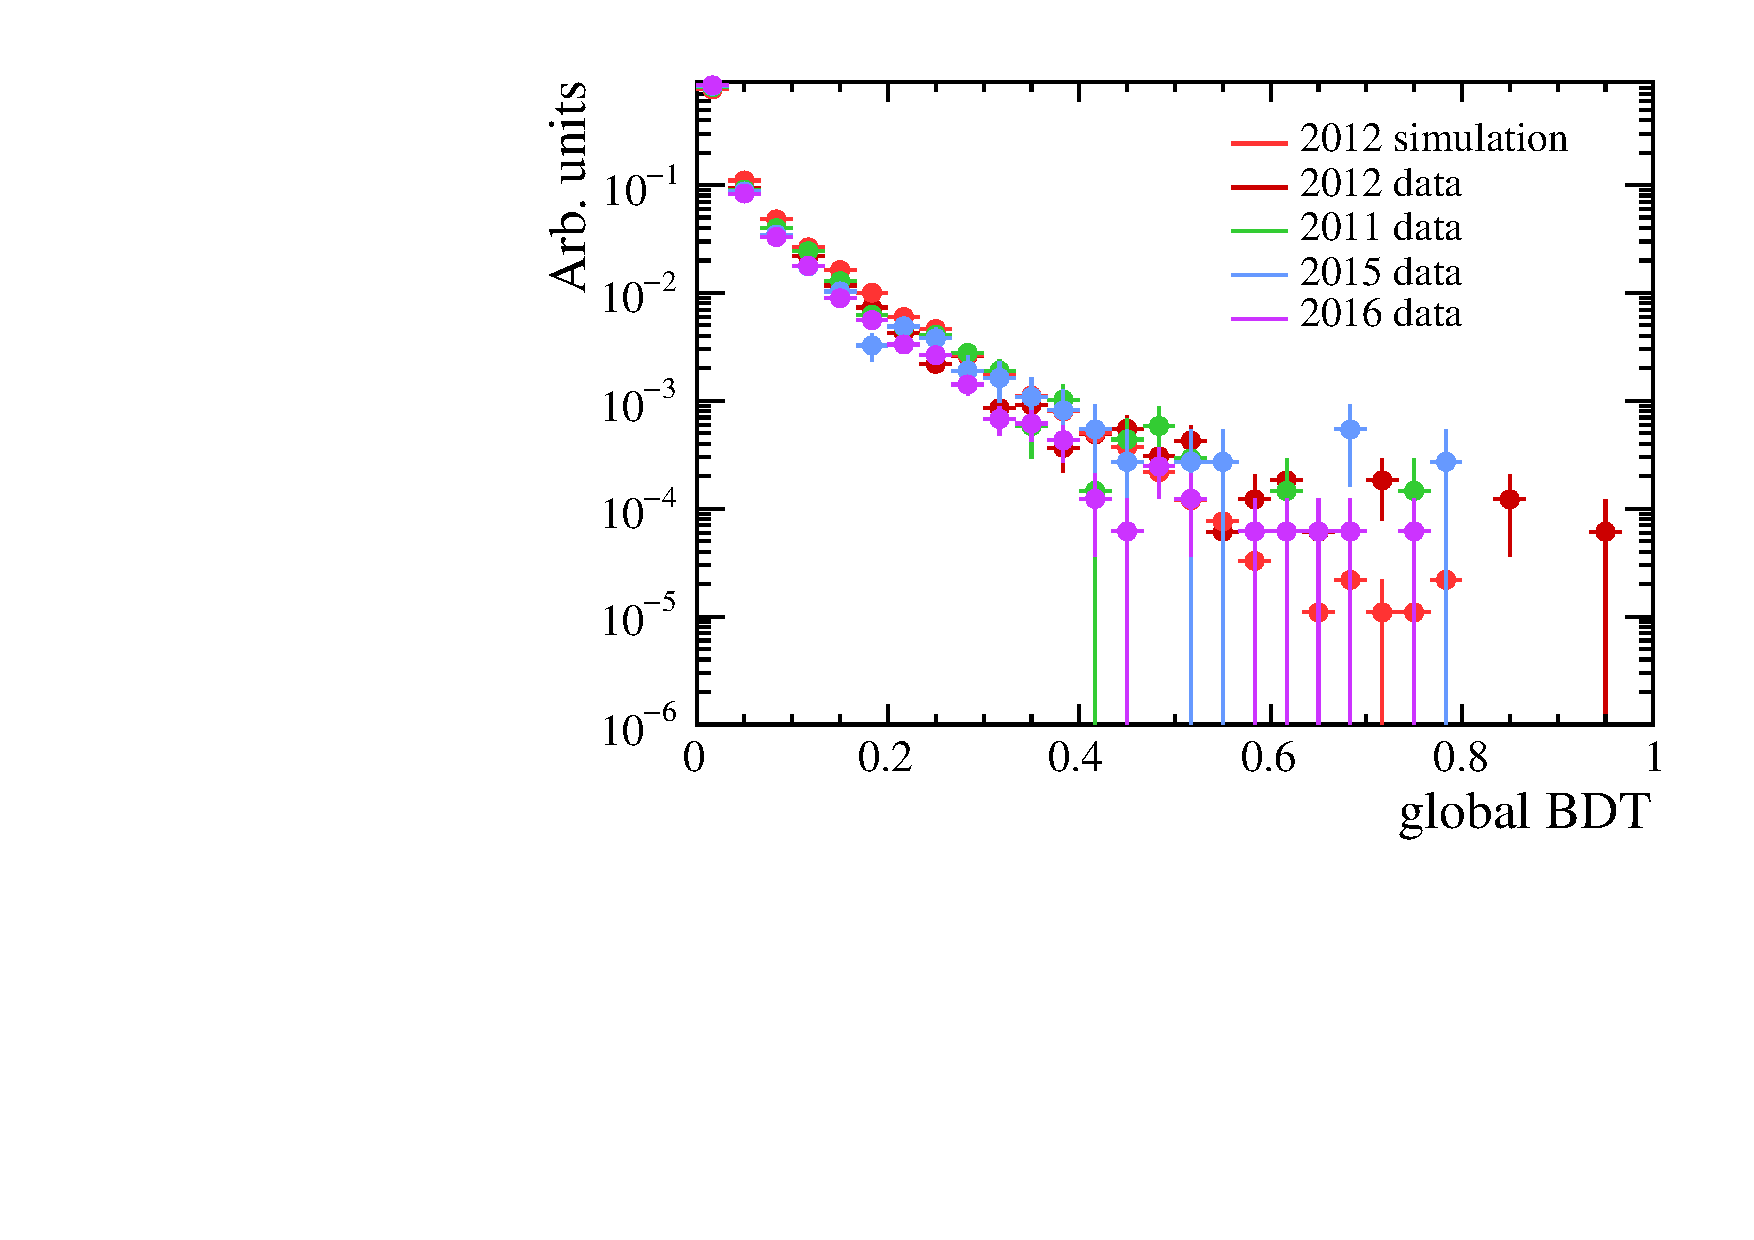
\includegraphics[width=\textwidth]{./Figs/Selection/BDTflat_bkgnd.pdf}
        %\caption{ }
        %\label{fig:BDTbkg}
    \end{subfigure}
    \caption{Global BDT output distributions for \bsmumu simulated decays (left) and \bbbarmumux decays from simulation and data.}
    \label{fig:FlatteningBDT}
\end{figure}


\begin{figure}[htbp]
    \centering
 \begin{subfigure}[b]{0.48\textwidth}
        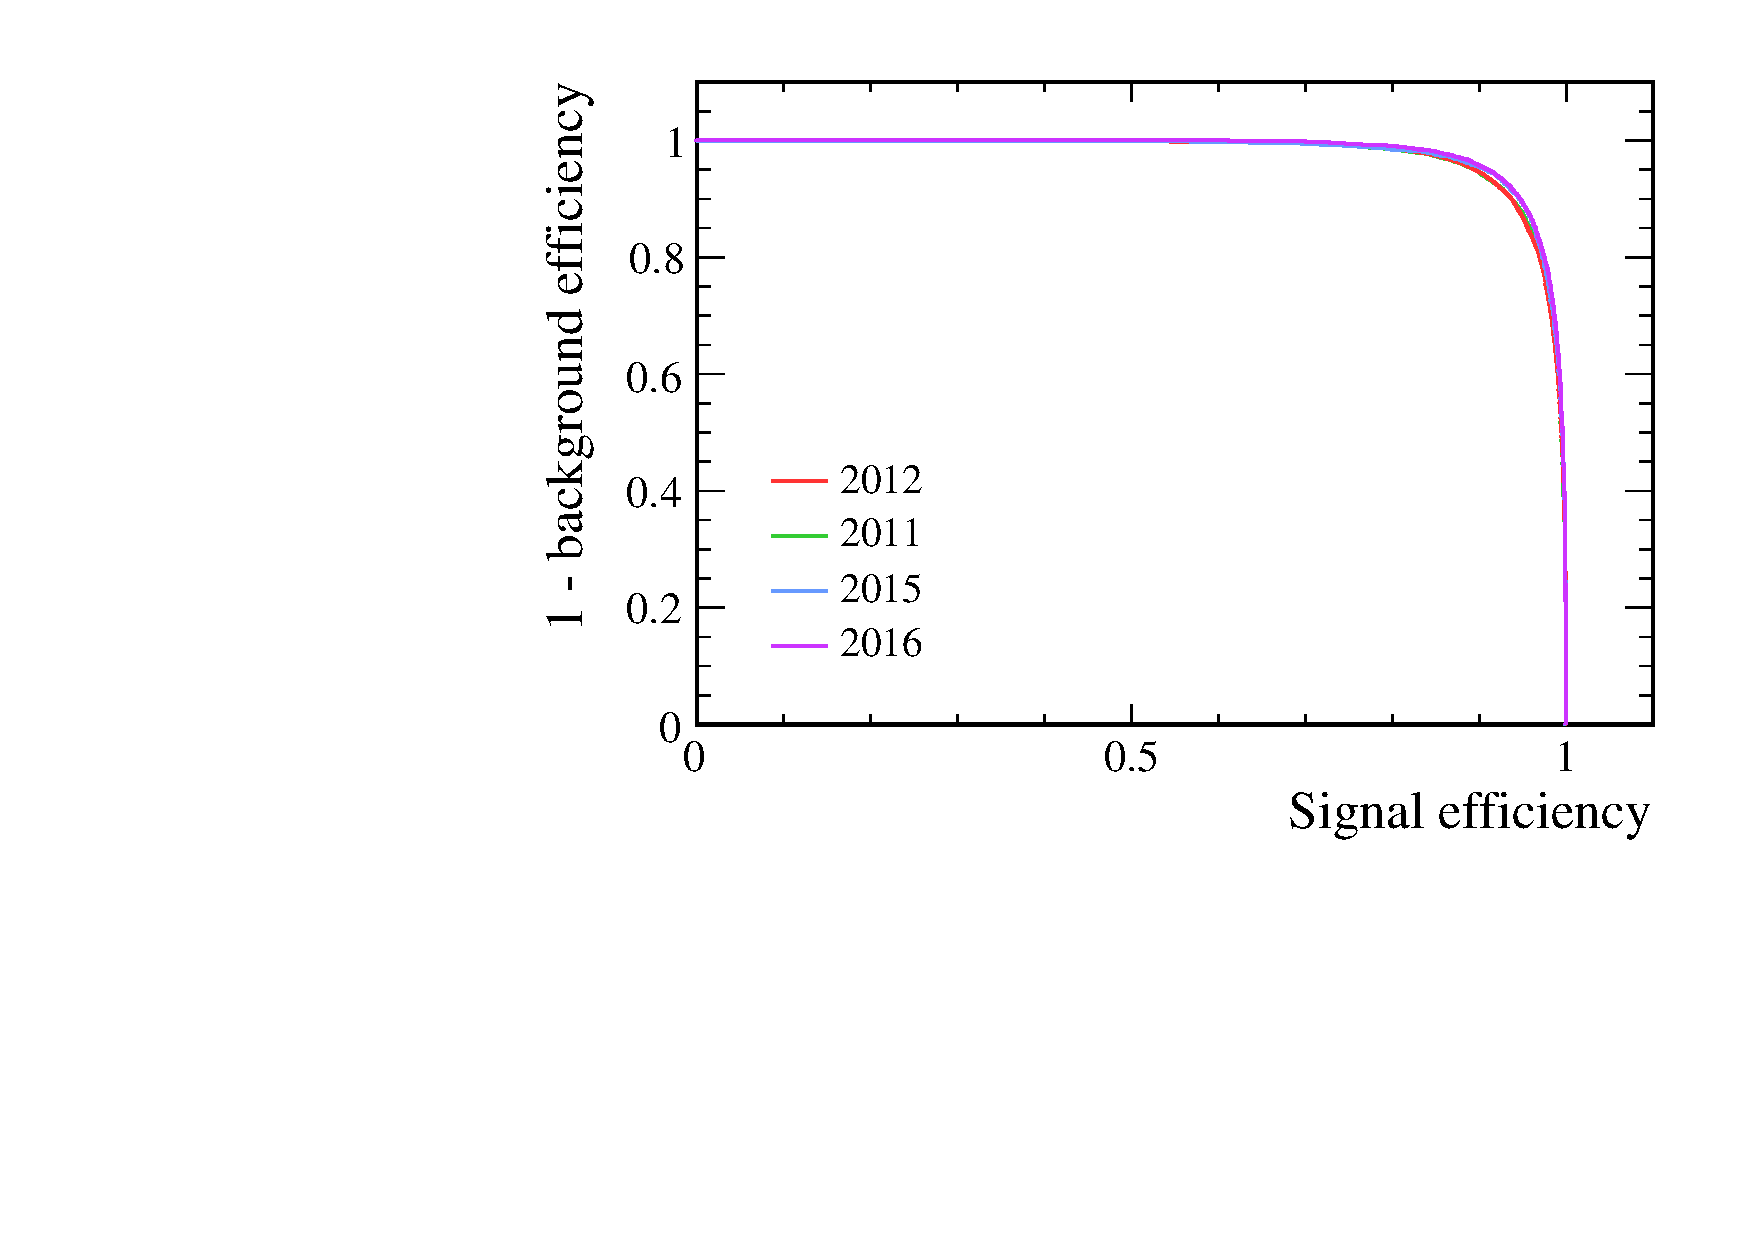
\includegraphics[width=\textwidth]{./Figs/Selection/ROC_full.pdf}
        %\caption{ }
        %\label{fig:ROCfull}
    \end{subfigure}
    ~ %add desired spacing between images, e. g. ~, \quad, \qquad, \hfill etc. 
      %(or a blank line to force the subfigure onto a new line)
    \begin{subfigure}[b]{0.48\textwidth}
       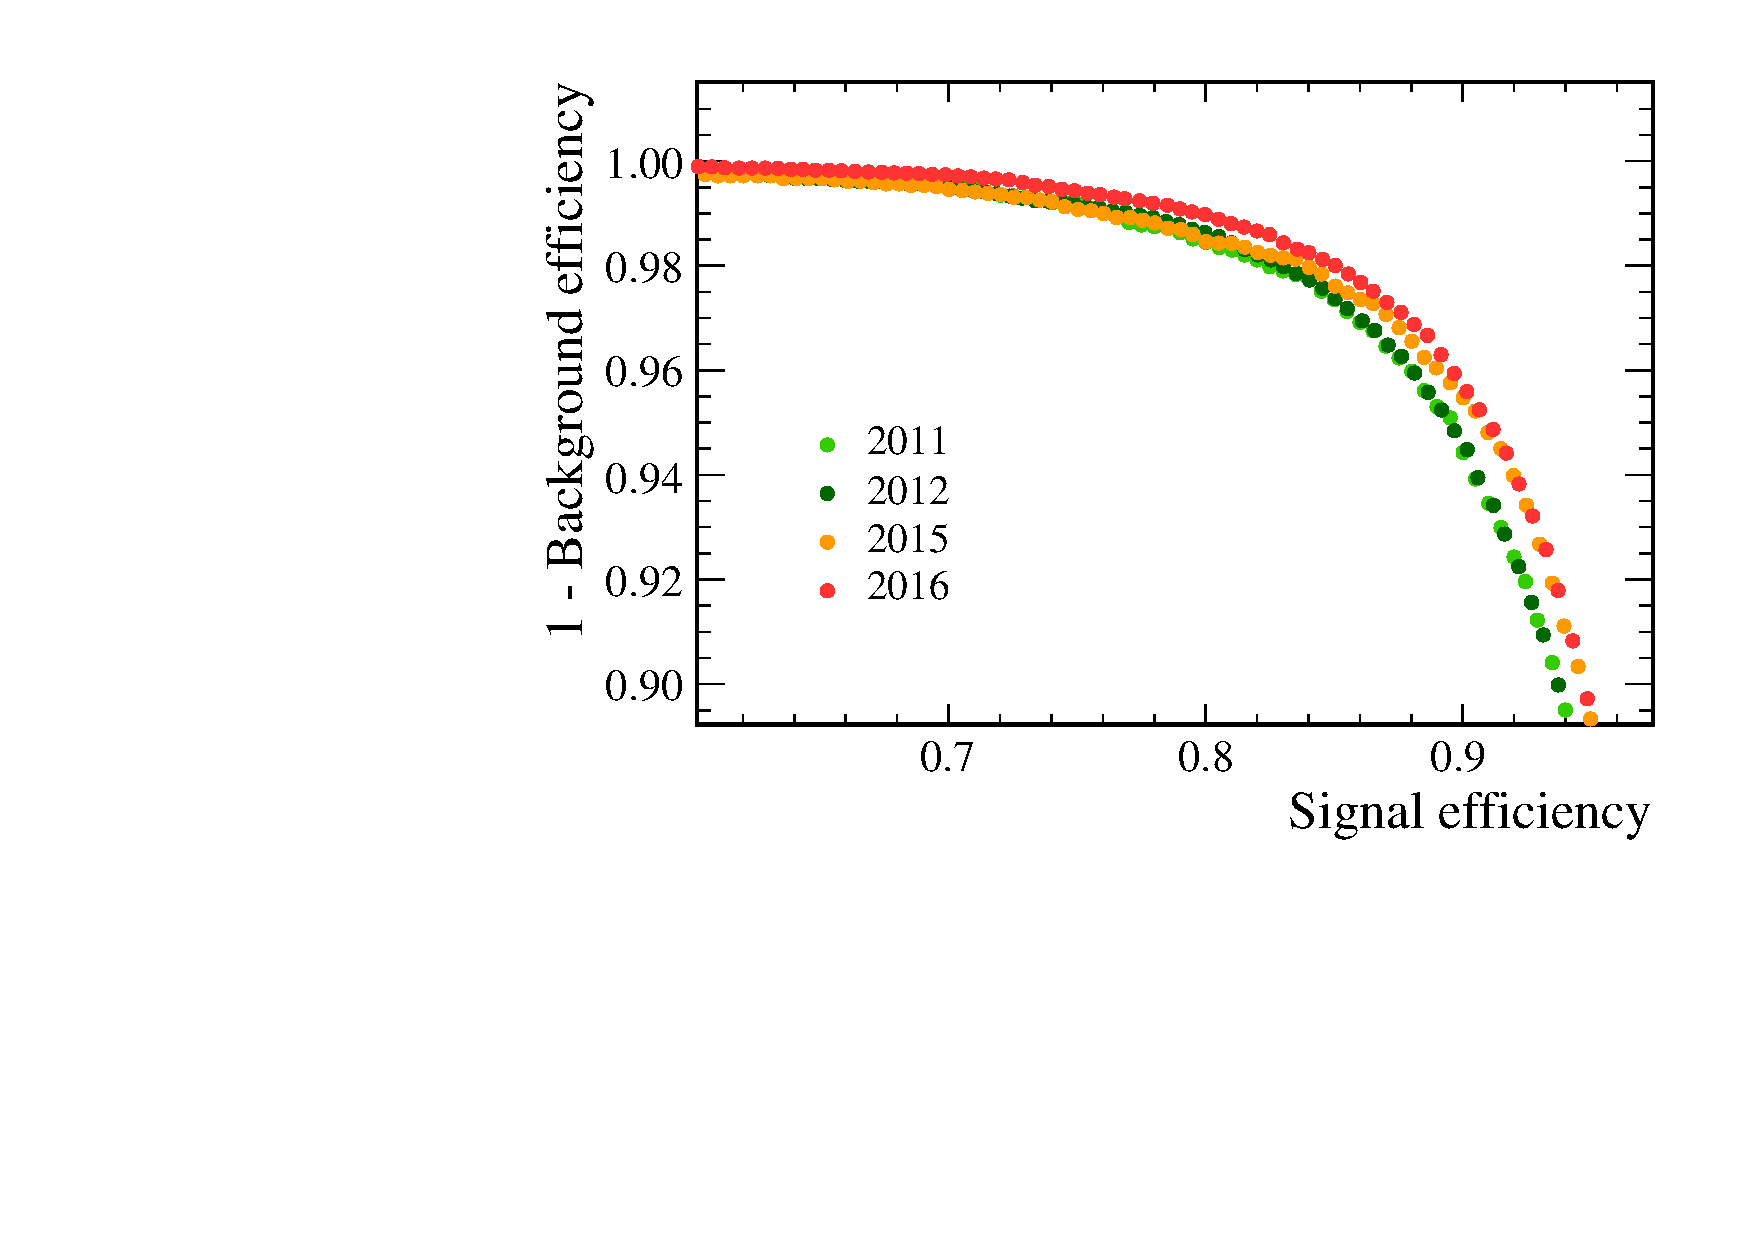
\includegraphics[width=\textwidth]{./Figs/Selection/ROC_zoom.pdf}
        %\caption{ }
        %\label{fig:ROCzoom}
    \end{subfigure}
        \caption{Global BDT performance for 2011, 2012, 2015 and 2016 data taking conditions. Signal efficiency is calculated from \bsmumu simulated decays and background rejection from data passing the \bsmumu selection with $m_{\mu^{+}\mu^{-}} > 5447$ \mevcc. The full BDT range is shown in the left plot and only the most sensitive region is shown in the right.}
    \label{fig:BDTperformance}
\end{figure}


\subsection{Summary}
\label{sec:BFsummary}
The complete set of selection criteria used for identify \bmumu decays in Run~1 and Run~2 data for the mesaurement of the \bmumu \BFs are listed in Tables~\ref{tab:fullpreselection}.% ands~\ref{} alongside the selection for \bhh, \bujpsik and \bsjpsiphi decays.
The selection requirements do not remove all backgrounds decays from the data set but reduce them to a level at whihc the \BFs can be measured. The selection criteria for \bhh and \bujpsik decays is kept as close as possible to that used to identify \bmumu decays in order to reduce systematic uncertainties from selection efficiencies in the noramlisation proceedure described in Section~\ref{sec:Normalisation}. 
%\begin{landscape}
%\vspace*{\fill}
\begin{table}[htbp]
\begin{center}
\begin{tabular}{ll}
\hline
Particle                & \bsmumu                              \\%        & \bhh                                 \\
\hline
\bs or $B^{+}$          & 4900 \mevcc $<$ M $<$ 6000 \mevcc     \\%         & 5000 \mevcc $<$ M $<$ 5800  \mevcc      \\                         
                        & DIRA $>$ 0                         \\%              & DIRA $>$ 0                             \\
                        & FD $\chi^{2}$ $>$ 225              \\%            & FD $\chi^{2}$ $>$ 225                  \\      
                        & IP $\chi^{2}$ $<$ 25             \\%              & IP $\chi^{2}$ $<$ 25                   \\
                        & Vertex $\chi^{2}$/ndof $<$ 9      \\%               & Vertex $\chi^{2}$/ndof $<$ 9              \\      
                        & DOCA $<$ 0.3 mm    \\%                            & DOCA $<$ 0.3 mm                          \\    
                        & $\tau$ $<$ 13.248 \ps  \\%                        & $\tau$ $<$ 13.248 \ps                \\
                        & $p_{T}$ $>$ 500 \mevc  \\%                         & $p_{T}$ $>$ 500 \mevc                \\%%
\hline
Daughter $\mu$ or $h$   & Track $\chi^{2}$/ndof $<$ 3 (4)   \\%               & Track $\chi^{2}$/ndof $<$ 3 (4)         \\                       
                        & Minimum IP $\chi^{2}$ $>$ 25 \\%                   & Minimum IP $\chi^{2}$ $>$ 25           \\             
                        & 0.25 \gevc $<$ $p_{T}$ $<$ 40 \gevc  \\%          & 0.25 \gevc $<$ $p_{T}$ $<$ 40 \gevc    \\
                        & $p$ $<$ 500 \gevc    \\%                            & $p$ $<$ 500 \gevc                       \\
                        & ghost probability $<$ 0.3 (0.4)     \\%           & ghost probability $<$ 0.3 (0.4)   \\    
                    & $|$m_{\mu\mu} - m_{\jpsi}$| $<$ 30$~\mevcc   \\%        &$|$m_{\mu\mu} - m_{\jpsi}$| $<$ 30$~\mevcc    \\
                        & isMuon = True               \\%                   &  -                                \\
                        & PID$_{\mu}$ > 0.4 (0.8)       \\%                  & -                 \\
\hline
                        & BDTS > 0.05             \\%                       &    BDTS > 0.05           \\                   

\hline
\end{tabular}
\vspace{0.7cm}
\caption{Selection cuts applied to select \bsmumu, where selection is different between Run~1 and Run~2 the Run~2 values are shown in parenthesis.}
\label{tab:fullpreselection}
\end{center}
\end{table}
%\vspace*{\fill}
%\end{landscape}

%\begin{landscape}
%\vspace*{\fill}
%\begin{table}[htbp]
%\begin{center}
%\begin{tabular}{lll}
%\hline
%Particle                & \bsmumu                                     & \bhh                                 \\
%\hline
%\bs or $B^{+}$          & 4900 \mevcc $<$ M $<$ 6000 \mevcc           & 5000 \mevcc $<$ M $<$ 5800  \mevcc      \\                         
%                        & DIRA $>$ 0                                    & DIRA $>$ 0                             \\
%                        & FD $\chi^{2}$ $>$ 225                       & FD $\chi^{2}$ $>$ 225                  \\      
%                        & IP $\chi^{2}$ $<$ 25                        & IP $\chi^{2}$ $<$ 25                   \\
%                        & Vertex $\chi^{2}$/ndof $<$ 9                  & Vertex $\chi^{2}$/ndof $<$ 9              \\      
%                        & DOCA $<$ 0.3 mm                             & DOCA $<$ 0.3 mm                          \\    
%                        & $\tau$ $<$ 13.248 \ps                       & $\tau$ $<$ 13.248 \ps                \\
%                        & $p_{T}$ $>$ 500 \mevc                        & $p_{T}$ $>$ 500 \mevc                \\%%
%\hline
%Daughter $\mu$ or $h$   & Track $\chi^{2}$/ndof $<$ 3 (4)               & Track $\chi^{2}$/ndof $<$ 3 (4)         \\                       
%                        & Minimum IP $\chi^{2}$ $>$ 25                 & Minimum IP $\chi^{2}$ $>$ 25           \\             
%                        & 0.25 \gevc $<$ $p_{T}$ $<$ 40 \gevc         & 0.25 \gevc $<$ $p_{T}$ $<$ 40 \gevc    \\
%                        & $p$ $<$ 500 \gevc                             & $p$ $<$ 500 \gevc                       \%\
%                        & ghost probability $<$ 0.3 (0.4)             & ghost probability $<$ 0.3 (0.4)   \\
%                        & $|$m_{\mu\mu} - m_{\jpsi}$| $<$ 30$~\mevcc        &$|$m_{\mu\mu} - m_{\jpsi}$| $<$ 30$~\mevcc    \\
%                        & isMuon = True                               &  -                                \\
%                        & PID$_{\mu}$ > 0.4 (0.8)                      & -                 \\
%\hline
%                        & BDTS > 0.05                                 &    BDTS > 0.05           \\                   

%\hline
%\end{tabular}
%\vspace{0.7cm}
%\caption{Selection cuts applied to select \bsmumu and \bhh decays, where selection is different between Run~1 and Run~2 the Run~2 values are shown in parenthesis.}
%\label{tab:fullpreselection}
%\end{center}
%\end{table}
%\vspace*{\fill}
%\end{landscape}



%\afterpage{
%\begin{landscape}
%\vspace*{\fill}
%\begin{table}[htbp]
%\begin{center}
%\begin{tabular}{l|l|l|l}
%\hline
%  Particle            &\bujpsik                             & Particle   &\bsjpsiphi \\
%\hline             
%$B^{+}$        & |M - M$_{PDG}$| $<$   500 \mevcc           & \bs         & |M - M$_{PDG}$| $<$   500 \mevcc       %      \\          
%                      & Vertex $\chi^{2}$/ndof < 45         &            &  Vertex $\chi^{2}$/ndof < 75         &  %  \\       
%                      & IP $\chi^{2}$ $<$ 25                &            &  IP $\chi^{2}$ $<$ 25               \\ %

%\hline   
%\jpsi                & |M - M$_{PDG}$| $<$   100 \mevcc      & \jpsi      &  |M - M$_{PDG}$| $<$   100 \mevcc     \\
%                    & DIRA > 0                             &           &   DIRA > 0           \\
%                    & FD $\chi^{2}$ $>$ 225                &           & FD $\chi^{2}$ $>$ 225        \\
%                    & Vertex $\chi^{2}$/ndof < 9           &           & Vertex $\chi^{2}$/ndof < 9       \\  
%                    &   DOCA $<$ 0.3 mm                   &            & DOCA $<$ 0.3 mm      \\  
%\hline             
%$\mu^{\pm}$               & Track $\chi^{2}$/ndof < 3           &$\mu$       &  Track $\chi^{2}$/ndof < 3 \\       
%                    & isMuon = True                      &            &isMuon = True    \\ 
%                    & Minimum IP $\chi^{2}$ $>$ 25        &            & Minimum IP $\chi^{2}$ $>$ 25    \\                   
%                    &  0.25 \gevc $<$ $p_{T}$            &            &  0.25 \gevc $<$ $p_{T}$    \\
%\hline
%$K^{+}$             & Track $\chi^{2}$/ndof < 3           & $\phi$           &  |M - M$_{PDG}$| $<$   20 \mevcc  \\
%                    & $p_{T}$ $>$ 0.25 \gevc              &           &  Minimum IP $\chi^{2}$ $>$ 4  \\
%                   & Minimum IP $\chi^{2}$ $>$ 25         & K$^{\pm}$           & Track $\chi^{2}$/ndof < 3  \\
%                  &                                     &                       & $p_{T}$ $>$ 0.25 \gevc     
%                        & BDTS > 0.05                                 &           \\                   
%\hline
%\end{tabular}
%\vspace{0.7cm}
%\caption{Selection requirements applied during the stripping selection for Run~1 data used in the \bmumu Branching Fraction analysis~\cite{CMS:2014xfa, Aaij:2013aka} to select \bujpsik and \sjpsiphi decays. $M_{PDG}$ corresponds to the Particle Data Group~\cite{Olive:2016xmw} mass of each particle.}%The track $\chi^{2}$/ndof and isMuon cut are applied during the reconstruction.}
%\label{tab:PreviousStripping}
%\end{center}
%\end{table}
%\vspace*{\fill}
%\end{landscape}
%}


\section{Candidate selection for the effective lifetime measurement}
\label{sec:ELsel}
The selection used to identify candidates for the measurement of the \bsmumu effective lifetime is based on the selection used to identify candidates for the measurement of the \bmumu \BFs. However several changes are made to account for the different measurement strategies that are descried in Chapeters~\ref{} and ~\ref{} and that only the \bs decay mode is required for the effective lifetime mesaurement. 
\bhh and \bsjpisphi decays are used to developed and validate the effective lifetime analysis strategy. The selection of \bsjpsiphi decays is kept the same as that used for the \BF measurement but there are a few differnces in the selection of \bhh decays for the effective lifetime measurement.

The majority of the selection of \bsmumu and \bhh decays is kept the same as the selection for the \BF measurement, the same cut based selection in Section~\ref{sec:cutbasedsel} is used and the BDTS requirement is applied.   
The differences in the selection are the trigger requirements, the mass ranges, the particle identification requirements and the use of the global BDT. The differences are outlined in the following sections and the full selection criteria are summaries in Section~\ref{sec:ELsummary}.


\subsection{Trigger}
\label{sec:ELtrigger}

The broad trigger lines L0Global, Hlt1Phys and Hlt2Phys, are used to selected \bsmumu candidates however different decisions made by these lines are used. Candidates are required to be TOS or TIS at each level of the trigger. The change in trigger decisions used for the effective lifetime analysis is motivated by the use of simulated decays in the measurement. The selection used to identify candidates is not uniform across the decay time range and the selection efficiency as a function of decay time is needed to measure the lifetime as describe in Section~\ref{}. Simulated \bsmumu decays are used in the determination of this efficency and in simulated data candidates that are triggerd by DEC decisions but are not included in TIS or TOS decisions are not well modelled. This arises due to the underlying event in simulated decays not accuratley describing data. Therefore these candidates are not used in data so to reduce the sysmtematic uncertainties from the evaluation of the selection efficency as a function of decay time. 
Candidates trigged by DEC decisions but not TIS or TOS do not pose the same problem for the \BF analysis because the selection and trigger efficiencies are evaluated using different methods as discussed in Section~\ref{}.

The analysis stragegy used to measure the \bsmumu effective lifetime is verifyied by measuring the lifetimes of \bdkpi and \bskk decays, that have already been accurately measured. Slightly different trigger decisions are used to select \bhh decays but the same trigger lines are used. To be useful as a validation channel the efficiency of the trigger requirements as a function of the decay time needs to be similar to the \bsmumu triggers, this is achieved by requiring \bhh decays to be TIS at each level of the trigger.

The requirements imposed on the trigger to select \bsmumu and \bhh decays is shown \
in Table~\ref{tab:ELtriggers}.

\begin{table}[htbp]
\begin{center}
\begin{tabular}{ll}
\hline
Trigger Line    & Trigger decision \\ \hline
%\multicolumn{2}{c}{{\it set A}} \\ \hline                                          
%L0Global       & Dec\\                                                             
%Hlt1Phys       & Dec \\                                                            
%Hlt2Phys       & Dec \\ \hline                                                     
\multicolumn{2}{c}{{\it Select \bsmumu decays}} \\ \hline
L0Global        & TIS or TOS \\
Hlt1Phys        & TIS or TOS \\
Hlt2Phys        & TIS or TOS \\ \hline
\multicolumn{2}{c}{{\it Select \bhh decays}} \\ \hline
L0Global        & TIS\\
Hlt1Phys        & TIS \\
Hlt2Phys        & TIS \\ \hline
\end{tabular}
\vspace{0.7cm}
\caption{Trigger lines used to select \bsmumu and \bhh decays for the \bsmumu effective lifetime analysis.}
\label{tab:ELtriggers}
\end{center}
\vspace{-1.0cm}
\end{table}


\subsection{Mass cuts}
\label{sec:ELmass}
The mass of \bsmumu candidates is restricted to the range 5320 - 6000 \mevcc, the motivation for the narrow mass window compared to the selection of candidates for the \BF analysis comes from the optimisation of the measurement strategy detailed in Section~\ref{sec:toys}. The lower mass bound now lies on the low edge of the \bs mass window, therefore \bdmumu candidatates and backgrounds from mis-identified \bhh and semi-leptonic decays are almost completely removed. Only background from random combinatations of muon in the events is left in the data set.  

\subsection{Particle identification}
\label{sec:ELpid}
The particle identification requirements used for selecting candidates for the mesurement of the \BF analysis were optimised to give the greatest sensitivity to \bdmumu decays. Backgrounds from \bhh and \lambdab decays pollute the \bd mass window and must be reduced as much as possible to enable good sennsitivity of \bdmumu decays. The requirement placed on the linear combination of ProbNN variables in Section~\ref{} is a comprimise between background rejcetion and signal efficiency. However for the measurement of the \bsmumu effective lifetime, the \bd mode is not relevant and the mass region of selected candidates removes the majority of \bdmumu decays and backgrounds from \bhh and \lambdab decays, therefore looser particle identification requrements can be used leading to a high efficiency to select signal decays.  

The same linear combination of ProbNN variables in Section~\ref{}, PID$_{\mu}$, is used because there is still a small contribution from mis-identified \bhh and \lambdab decays that can be reduced and in addition the particle identification requirements help to reduce the number of combinatorial background decays. Different ProbNN tunes and consequently cut values are used for Run 1 and 2015 data compared to 2016 data. The cuts are chosen to give similar efficiencies for each data set at selecting signal and removing background and are listed in Table~\ref{}. The cut values have not been optimised because there are too few candidates in data after the selection to enable this and simulated decays are not used because particle identification variables are not well modelled in simulation. However the particle identification requirement are still tight enough to make the expected number of mis-identified decays in the data set after the full selection negliable, as shown in Section~\ref{}. 
%Maybe some PID plots?
The validation of the measurement strategy of the \bsmumu effective lifetime is done by measuring the lifetimes of \bdkpi and \bskk decays. The selection of these two \bhh decays is identical until the particle identification requirements, where different decay modes are seperated via DLL$_{K}$ variable. The DLL variables are useful to separate \bhh decays where $h$ is either a pion or kaon because the variables compare different particle hypotheses with the pion hypotheses. The selection requirements used are given in Table~\ref{} and are the same for each year of data taking.


\begin{table}[htbp]
\begin{center}
\begin{tabular}{lll}
\hline
Decay                    & Particle               & PID requirements \\
\hline
\bsmumu  (Run~1 and 2015) & PID$_{\mu}$ > 0.2 \\
\bsmumu  (2016)          & PID$_{\mu}$ > 0.4 \\
\bdkpi and \bskpi       & $K^{+}$                & DLL$_{K\pi}$ $>$ 10 \\
                         & $\pi{-}$              & DLL$_{K\pi}$ $<$ -10 \\
\bskk                    & $K^{+}$ and $K^{-}$    & DLL$_{K\pi}$ $>$ 10 \\
\hline
\end{tabular}
\vspace{0.7cm}
\vspace{0.7cm}
\caption{Particle identification requirements to select \bsmumu decays and to separate the \bhh decays \bdkpi and \bskpi from \bskk. }
\label{tab:PID}
\end{center}
\vspace{-1.0cm}
\end{table}


\subsection{MVA}
\label{sec:ELmva}
The selection of canddiates for the measurements of the \bmumu \BF uses two multivariate classifiers to seperate signal and combinatorial background decays. The BDTS is used first to remove candidates that are very unlikely to be signal and to reduce the size of the data set. The global BDT is then used to classify candidates in to bins of BDT and a simultaneous fit it then applied accorss the BDT bin to measure the \BFs, this proceedure is described in Chapter~\ref{}. 

A different, simpler strategy is use to identify candidates for the measurement of the \bsmumu effective lifetime. Combinatorial backgrounds are reduced by placing a cut on the output of a multivariate classifier, then all candidates passing the selection cut are used to measure the \el. The measurement strategy that motivates this selection proceedure is detailed in Chapter~\ref{}. 

As a consequence of the different selection method, two classifiers may not be necessary for the measurement of the \el. Therefore alternative classifiers were developed in parallel to the development of the global BDT and the performance was compated to detemine the most effective way to select candidates for the \bsmumu \el measurement. 

\subsubsection{Developement of \el multivarite classifiers}

Several different types of multivarite classifiers were investigated for the effective lifetime selection and boosted decision trees gave the best performance at seperating signal and from background. A range of boosting methods for the decision trees were studies and the Adaptive boosting method, once again, yielded the best results. %Do I mention the Grad method? I don't think it adds anything but I did study it quite a lot. 
However a boosting method of particular interest of the effective lifetime measurement was the uBoost technique~\ref{}. The uBoost method produces a classifier output that has a uniform efficiency for a specified variable. The selection used to identify \bsmumu candidates uses variables that are correlated with the decay time of the \bs in the stripping selection and the most effective input variables for BDTs are also correlated with the decay time. Therefore the overall selection efficiency varies as a function of decay time. The final measurement of the \bsmumu \el relies of the efficiency being well understood. This is described in detail in Section~\ref{}. If the output of a BDT is correlated with the \bs decay time the efficiency as a function of decay time may not have a smooth or easily understandable distribution, the uBoost method could provide a way to make modelling the efficiency as a function of decay time easier by requiring the algorithm output has a uniform efficiency across the decay time distribution.

Simulated 2012 \bsmumu decays were used as the signal training sample for the BDTs and two different samples were used for the background training sample. One sample consistented of simulated 2012 \bbbarmumux decays and the other was combinatorial background decays in Run 1 data. At the time of BDT development only Run~1 data was avaliable. The selection requirements listed in Table~\ref{}, except the BDTS requirement, were applied to training samples of simulated decays and combinatorial background decays in data were identified as candidates that pass the selection requirements listed in Table~\ref{}, except the BDTS requirement and with by having a dimuon invaraint mass in the range 5447 - 6500 \mevcc, outside to the \bs mass window. 

The input variables used in the adaptive boosting and uBoost BDTs were chosen seperately starting from a large set of variables including kinematic, geometric and isolation variables. Initially the BDTs were trained using all input variables within the set and variables were removed that had no impact on the performance of the BDT until removing any of the remaining variables had a negative impact on the BDT performance. The final varible sets were different for the two boosting methods; the adaptive boosting BDT (aBDT) uses X input variables and the uBoost BDT (uBDT) uses Y input variables. The full list of input variables used and the definition of those variables are given in Appendix~\ref{}. 

The performance of the BDT with different boosting methods and trained using simulated decays and data as the background decays was evaluated using \bhh decays in data. No particle identification variables were used in the input variables of the BDTs due to the incorrect modelling of particle identification variables in simulated decays, therefore the performance on the BDTs on \bhh decays should be very similar to \bsmumu decays. \bhh decays in data were identified by passing the standard \bhh selection in Table~\ref{} and the trigger requirements used to select \bsmumu decays for the branching fraction analysis, no particle identification requirements were used to seperate different \bhh decays. An unbinned \ml fit was applied to the \bhh mass distribution, where all \bhh decays are reconstructed as \bsmumu, for a range cuts on the BDT outputs and the signal significance $\mathcal{S}$  was evaluated for each cut on the BDT output. In the \ml fit the \bhh mass distribution was modelled with a Gaussian function and the combinatorial background decays with an exponential, an example of the mass fit is given in Figure~\ref{}. The signal signficance is given by
\begin{equation}
\mathcal{S} = \frac{S}{sqrt{S+B}}
\label{eq:SigSigf}
\end{equation} 
where S (B) are the number of signal (background) decays within 3 $\sigma$ of the center of the \bhh mass peak. 
The signal significance as a function of the cut value placed on the BDT output for the different BDTs trained on data and simulated decays for the background samples are shown in Figure~\ref{}. The outputs of the BDTs are not flattened, aBDT gives output values between -1 and +1 and uBDT gives output values between 0 and +1. It is clear from Figure~\ref{} that the performance of BDTs trained on simulated decays is better that that of the BDTs trained on data, this is due to the higher statistics avaliable for simulated decays. The number of decays used in the training samples after the selection requirements are shown in Table~\ref{}. Furthermore the performance of aBDT is better that uBDT which is expected because the adpative BDT is not constrained to have a uniform efficiency across the decay time range. 

Both the adaptive and uBoost BDTs shown in Figure~\ref{} were trained without applying the BDTS cut to the training samples, however the signal significance on \bhh decays has been revaluated with not BDTS cut applied, with the BDTS cut applied after the BDT training and before the BDT training. The improvement in the overall performances of the BDTs is small but appling the BDTS cut to \bhh as well as the BDT given the highest signal significances. 

The training parameters of the adaptive BDT have been optimised by iterating over a large range of different values, whereas the training parameters of the uBoost were not optimised because changing the parameters has a small impact of the overall BDT performance~\cite{}. The values used are given in Appendix~\ref{}. 

The understanding of the selection efficiency as a function of decay time was the main motivation for investigating the uBoost boosting method. The performance of the uBoost boosting method is quite a lot worse than the adaptive BDT method. The selection efficiency as a function of decay time has been evalutated in simulated \bsmumu decays after the all selection requirements and a range of different cut values on the outputs of the adaptive and uBoost BDTs trained on simulated decays. The cut values are chosen to have the same selection efficiencies for each algorithm. The efficiencies are shown in Figure~\ref{}, although the shapes are quite different the unifrom efficiecny of the uBoost BDT is evident. The adaptive BDT removes a greater proportion of decays at low decay time than the uBoost method. Ideally, to reduce systematic uncertainties on the measurement of the effective lifetime, the selection would not bias the decay time distribution, however with the expected statistics of the data set an unbiased selection would not be approtriate. However the efficienciy of the adaptive boost BDT is smooth across the decay time range and therefore using that algorithm would not cause any sever problems. 


\subsubsection{Classifer performance}

The final classifer for the selection of \bsmumu candidates has the greatest seperation powers between signal and combinatorial background decays, it will be the classifier that removes the most combinatorial backgound decays for a given signal efficiency. The performance of the two BDTs developed specifically for the effective lifetime measurement is compared to that of the global BDT used to classify candidates for the branching fraction measurements. Two different approaches are used to evaluate the performances. The output of the two BDTs developed for the effective lifetime selection have been flattened like the global BDT to enable easy comparison.

The signal significance for each BDT is evaluates on \bhh decays in Run 1 data and the maximum signal significance in found. The BDTS cut is applied in the selection process because the global BDT was designed to be used with the BDTS and the performance of the BDTs developed for the effective lifetime is best when the BDTS requirement is used. The results are shown in Figure~\ref{}, the global BDT produces the highest signal significance but is closely followed by the adaptive BDT developed for the effective lifetime measurement. 

However since the purpose of the BDT is to remove combinatorial background decays passing the \bsmumu selection and additional comparsion of the different algorithms is made. The number of combinatorial background decays present in Run 1 data passing the \bsmumu selection in Table~\ref{} but in the mass range 5447 - 6550 \mevcc is found for a range of cuts to the output of the three BDTs. No particle identification requirements are applied. The cut values are chosen seperatly for each algoithm so that the number of background decays is found for cuts with the same efficiency for selecting \bsmumu decays. The results are given in Table~\ref{} and the global BDT is most effective at removing background decays for a given signal efficiency.

\begin{table}[htbp]
\begin{center}
\begin{tabular}{l|cccccccccc}
\hline
BDT & \multicolumn{}{c}{Number events above BDT output value}  \\
   & 0.1 & 0.2 & 0.3 & 0.4 & 0.5 & 0.6 & 0.7 & 0.8 & 0.9 \\
Global BDT & 2618 & 717 & 293 & 116 & 51 & 23 & 8 & 3 & 1 \\
Adaptive BDT & 5445 & 1717 & 647 & 290 &106 & 49 & 21 & 8 & 3 \\
uBoost BDT & 8967 & 3742 & 1718 & 707 & 298 & 104 & 33 & 10 & 1 \\
\hline
\end{tabular}
\vspace{0.7cm}
\vspace{0.7cm}
\caption{Number of candidates in passing the \bsmumu selection in the mass range 5447 - 6000 \mevcc, the selected is loosened so that no particle identification requirements are applied and the loosest trigger requirements are used, requiring DEC at each level of the trigger. }
\label{tab:bkgds}
\end{center}
\vspace{-1.0cm}
\end{table}


\begin{table}[htbp]
\begin{center}
\begin{tabular}{l|cccccccccc}
\hline
BDT & \multicolumn{}{c}{Number events above BDT output value}  \\
   & 0.1 & 0.2 & 0.3 & 0.4 & 0.5 & 0.6 & 0.7 & 0.8 & 0.9 \\
Global BDT & 2618 & 717 & 293 & 116 & 51 & 23 & 8 & 3 & 1 \\
Adaptive BDT & 5445 & 1717 & 647 & 290 &106 & 49 & 21 & 8 & 3 \\
uBoost BDT & 8967 & 3742 & 1718 & 707 & 298 & 104 & 33 & 10 & 1 \\
\hline
\end{tabular}
\vspace{0.7cm}
\vspace{0.7cm}
\caption{Number of candidates in passing the \bsmumu selection in the mass range 5447 - 6000 \mevcc, the selected is loosened so that no particle identification requirements are applied and the effective lifetime triggerers are used. }
\label{tab:bkgdsB}
\end{center}
\vspace{-1.0cm}
\end{table}

\begin{table}[htbp]
\begin{center}
\begin{tabular}{l|cccccccccc}
\hline
BDT & \multicolumn{}{c}{Number events above BDT output value}  \\
   & 0.1 & 0.2 & 0.3 & 0.4 & 0.5 & 0.6 & 0.7 & 0.8 & 0.9 \\
Global BDT & 
Adaptive BDT &
uBoost BDT & 
\hline
\end{tabular}
\vspace{0.7cm}
\vspace{0.7cm}
\caption{Number of candidates in passing the \bsmumu selection in the mass range 5447 - 6000 \mevcc, the selected is loosened so that particle identification requirements are applied and the effective lifetime triggerers are used. }
\label{tab:bkgdsC}
\end{center}
\vspace{-1.0cm}
\end{table}


Although the global BDT combined with the BDTS performs best at seperating signal from background decays, the efficiency as a function of decay time must also be evalutes for these alorithms to ensure it does not exhibit any strange behaviour. The decay time efficiency is shown in Figure~\ref{} for several BDT cut values and gives a smooth distribution as a function of decay time. For the data set used to measure the \bsmumu effective lifetime the expected number of \bsmumu decays is very low, therefore the benefits of using the uBoost method are outweighting by its poor performance. Therefore the global BDT developed for the the \BF is the best BDT to use for the selection of events for the \bsmumu effective lifetime. 

\subsubsection{Global BDT choice}
\label{sec:globalBDToptimisation}

A cut is place on the output of the global BDT to select \bsmumu decays. The cut value has been optimised to give the smallest expected uncertainty on the measurement of the \bsmumu effective lifetime, \tmumu, and its inverse, \invtmumu. This is done by using toy experiments for the expected number of \bsmumu combinatorial background decays for different cut on the global BDT output. The same global BDT cut is used to select \bhh decays to verify the analysis stragegy to measure \tmumu.

The fit procedure to extract \tmumu from the data is described in depth in Chapter X along with a discussion of whether it is best to fit for \tmumu or \invtmumu. The toy experiment used to optimise the global BDT cut value are preformed following the steps;
\begin{itemize}
\item the mass and decay time distribution for number of expected \bsmumu and combinatorial background events are generated using the expected mass and decay time probability density functions
\item an unbinned maximum likelihood fit is performed to the dimuon invariant mass spectrum, where the \bsmumu and combinatorial background yields are free to float in the fit along with the slope of the combinatorial background mass distribution c
\item the mass fit is used to compute sWeights using the sPlot method \cite{Pivk:2004ty}
\item a maximum likelihood fit is performed to the sWeighted decay time distribution to extract \tmumu and \invtmumu. 
\end{itemize}
Full details of the toy experiment set up and the probability density functions used are given in Appendix X. 

The number of expected \bsmumu and combinatorial background events for different BDT cut values is derived from the expected number of decays passing in the all the selection cuts and BDT $>$ 0.55 for Run~1 and Run~2 data but in the mass range 4900 $<$ $m_{\mu^{+}\mu^{-}$ $<$ 6000 \mevcc. These predictions assume the SM branching fraction for \bsmumu and are given in Table~\ref{tab:expectednumbers}. Since the output of the global BDT is flattened the number of \bsmumu decays is evenly distributed across the BDT range, therefore the expected number of \bsmumu decays is straight forward to calculated for each BDT cut value. The number of combinatorial background decays expected after each BDT is is computed from simulated \bbbarmumux decays using the ratio
\begin{equation}
R = \frac{\epsilon(BDT > X)}{\epsilon(BDT > 0.55)}
\end{equation}
where $\epsilon(BDT > X)$ is the efficiency of the cuts BDT $>$ X. The \bsmumu selection requirements are applied to the simulated decays before taking the efficiency. The ratios for the different cuts values are shown in Table~\ref{tab:EfficiencyRatioCombBG}. Simulated decays had to be used to compute the efficiencies rather than data because there were too few candidates left after the higher BDT cuts were applied to data to enable meaningful studies. 




\begin{table}[htbp]
\begin{center}
\begin{tabular}{lc}
\hline
Decay & Expected number of candidates \\ \hline
\bsmumu & 30.94 \\
Combinatorial background & 66.23\\
\hline
Total & 97.17\\
\hline
\end{tabular}
\vspace{0.7cm}
\caption{Expected number of \bsmumu and combinatorial background candidates after the \bsmumu selection requirement and with a global BDT value greater than 0.55 in the mass range 4900 $< m_{\mu^{+}\mu^{-}} <$ 6000 \mevcc. }
\label{tab:expectednumbers}
\end{center}
\vspace{-1.0cm}
\end{table}

\begin{table}[htbp]
\begin{center}
\begin{tabular}{lc}
\hline
Global BDT cut & $R_{\epsilon}$ \\ \hline 
0.40 & 8.69 \\
0.45 & 3.91 \\
0.50 & 1.91 \\
0.55 & 1.00 \\
0.60 & 0.55 \\
0.65 & 0.32 \\ \hline
\end{tabular}
\vspace{0.7cm}

\caption{The ratio of efficiencies of cuts on the global BDT to select \bbbarmumux decays relative to a cut of 0.55 on the global BDT. }
\label{tab:EfficiencyRatioCombBG}
\end{center}
\vspace{-1.0cm}
\end{table}


The mass distribution of the combinatorial background is a decaying exponential, it was observed from the simulated \bbbarmumux decays that the slope of the mass distribution changed with the BDT cut value as illustrated in Figure~\ref{fig:BDTmasses}. The change in slope is accounted for when generating events for the toy experiment by changing the slope parameter ($\lambda$) for each BDT cut. Table~\ref{tab:CBGSlopeBDT} shows the slope of the mass distribution for different BDT cuts values evaluated from \bbbarmumux simulated decays.

\begin{figure}[htbp]
    \centering
    \begin{subfigure}[b]{0.7\textwidth}
        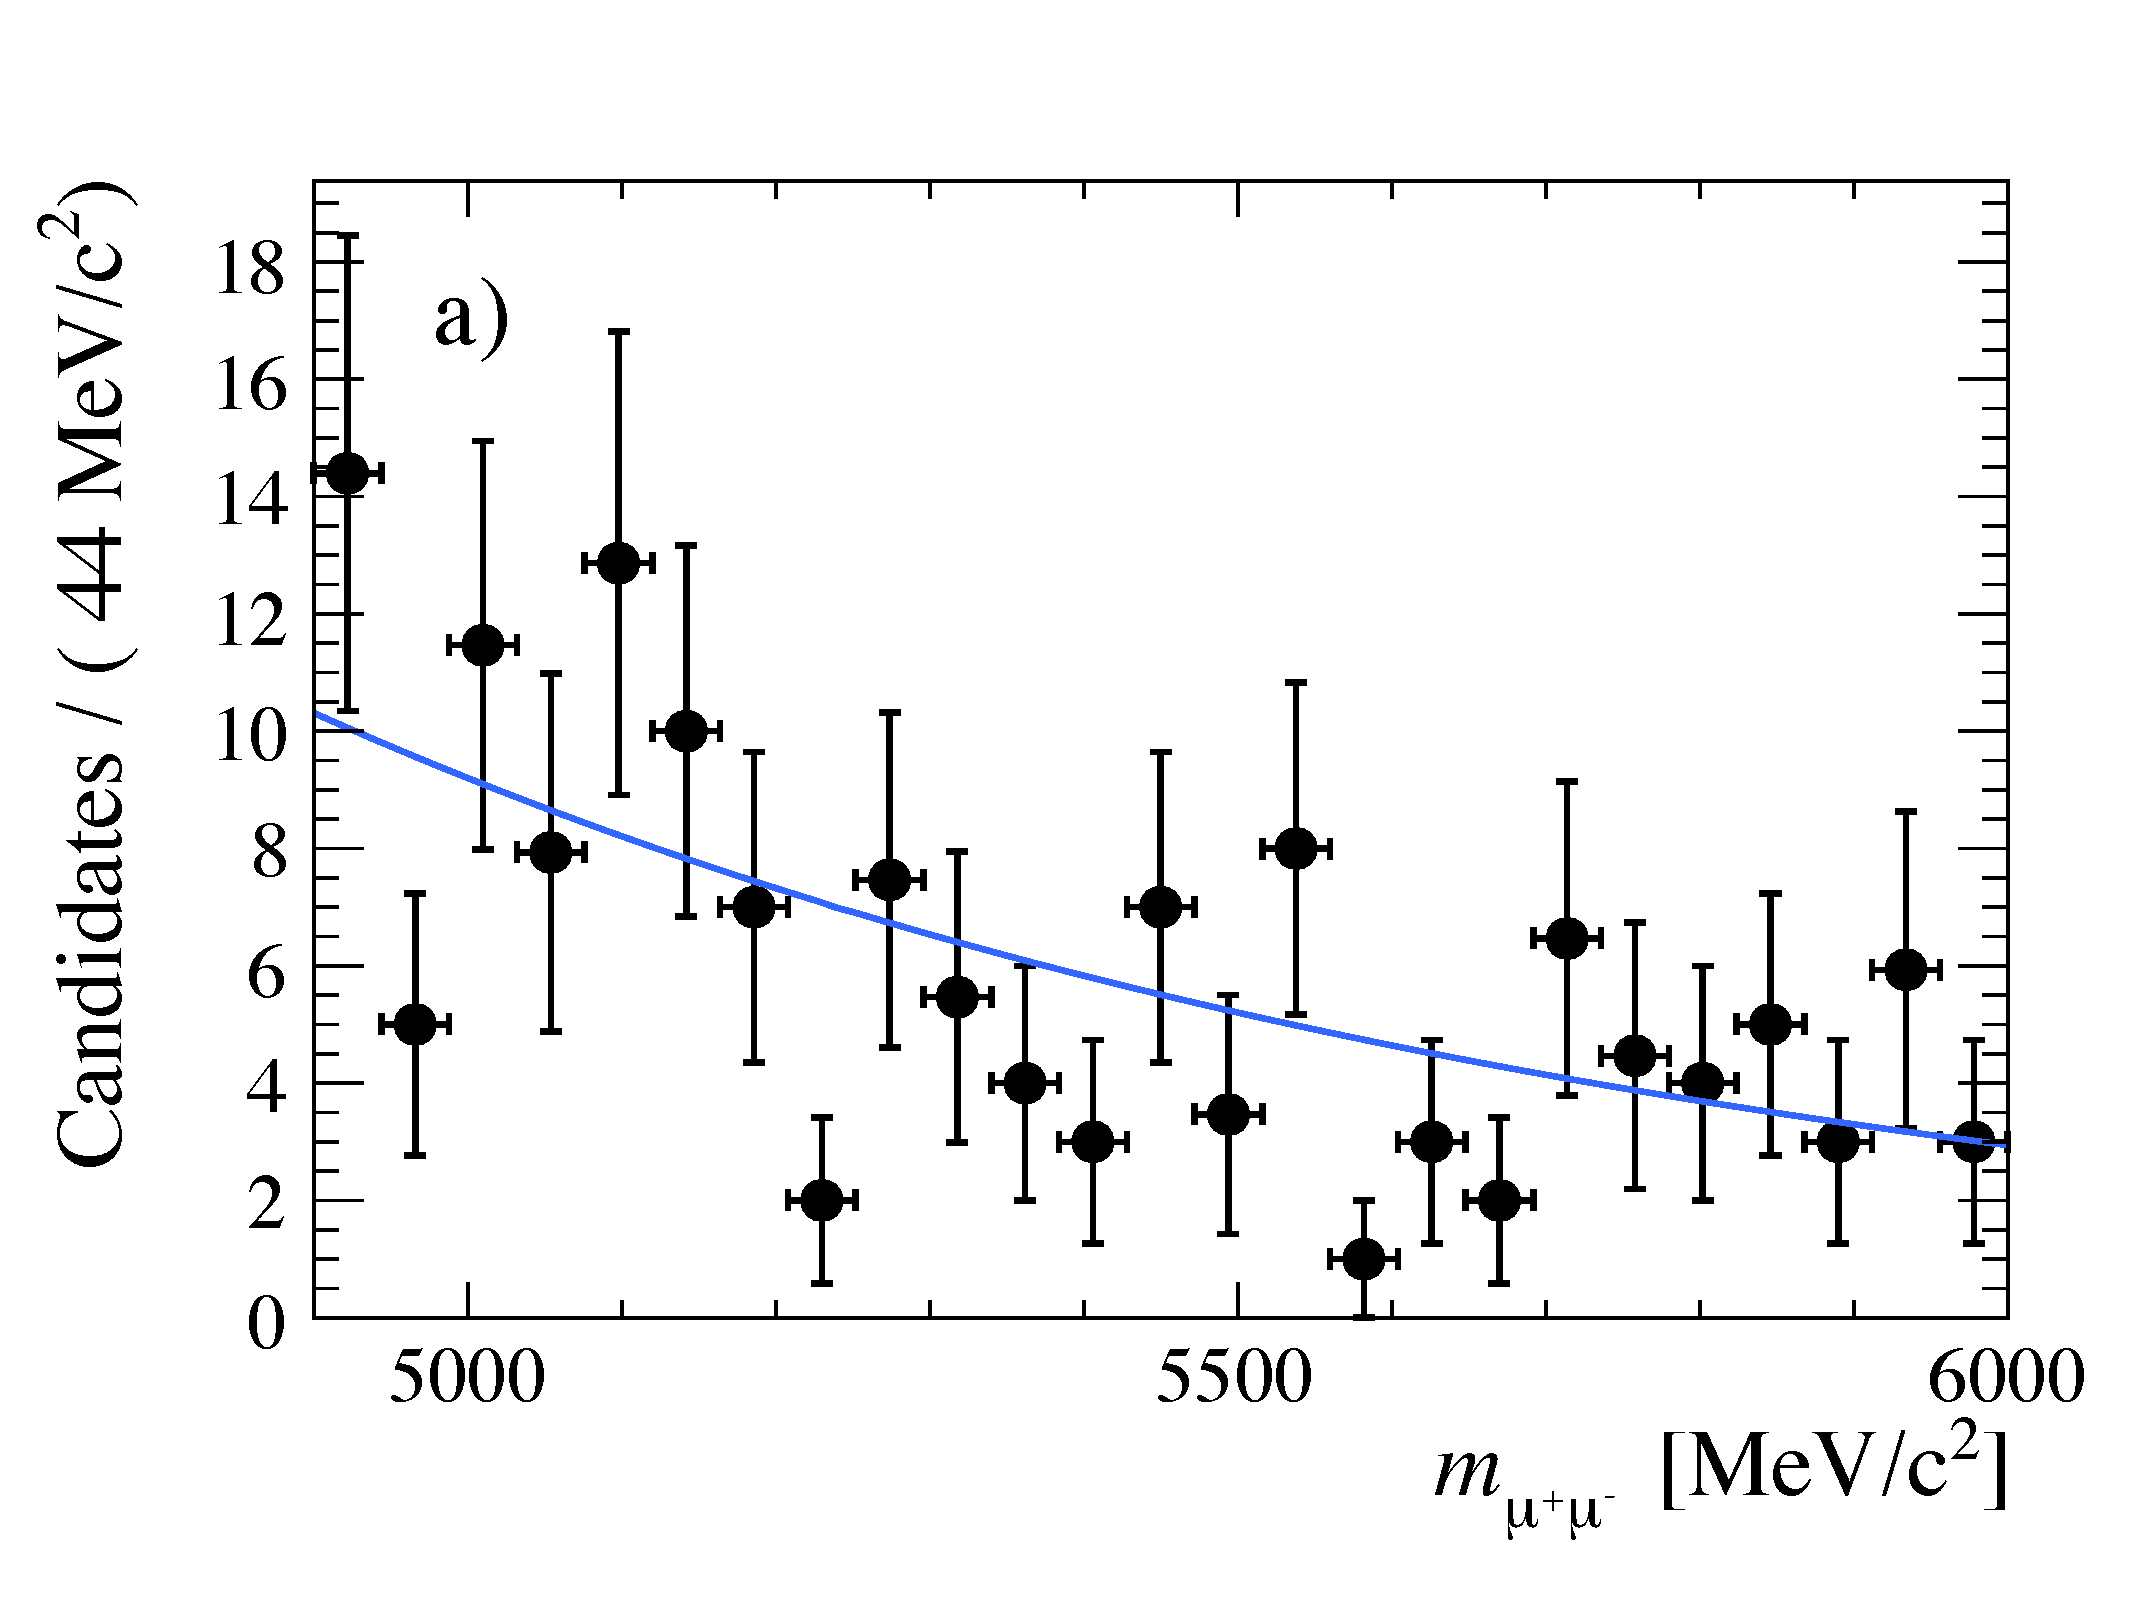
\includegraphics[width=\textwidth]{./Figs/Selection/BDT0p4.pdf}
        \caption{ }
        \label{fig:BDT0p4}
    \end{subfigure}
    ~ %add desired spacing between images, e. g. ~, \quad, \qquad, \hfill etc. 
      %(or a blank line to force the subfigure onto a new line)
    \begin{subfigure}[b]{0.7\textwidth}
       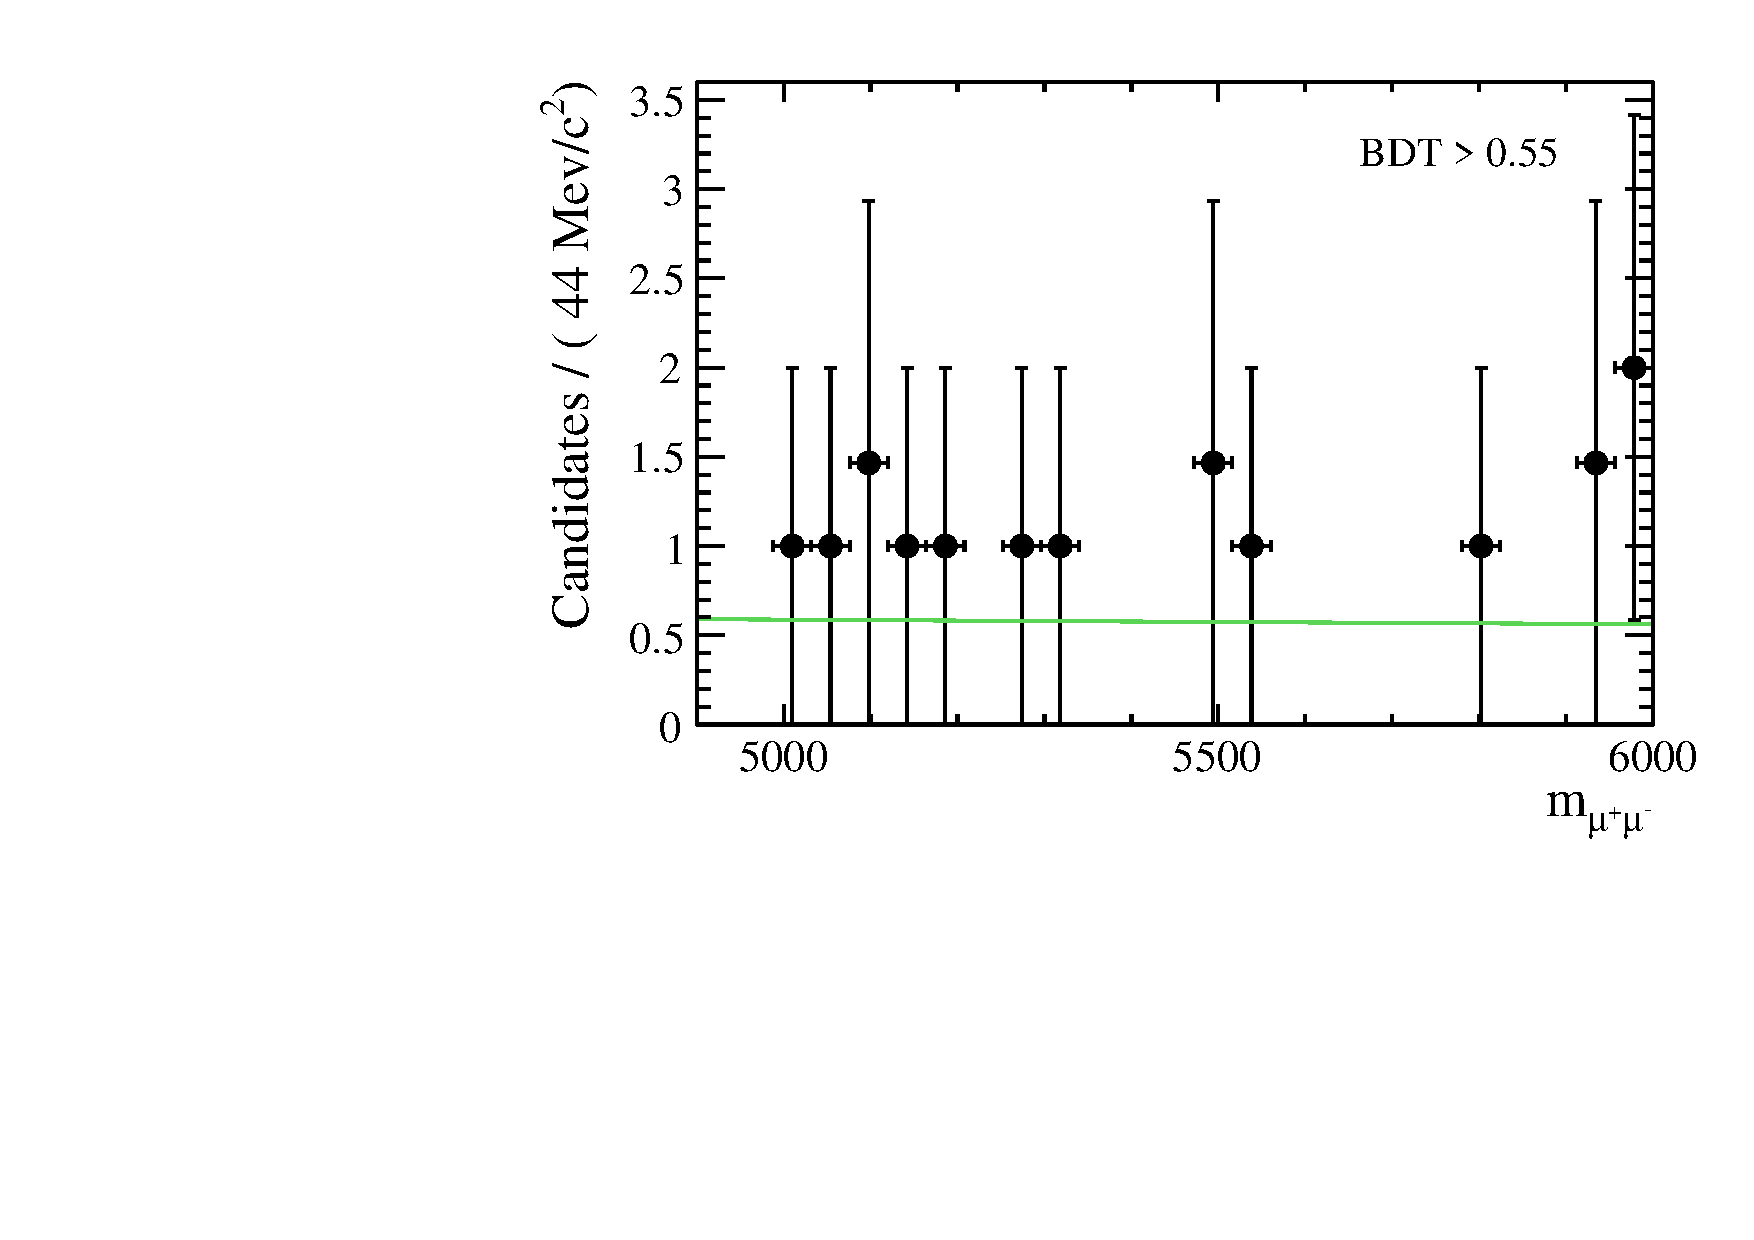
\includegraphics[width=\textwidth]{./Figs/Selection/BDT0p55.pdf}
        \caption{ }
        \label{fig:BDT0p5}
    \end{subfigure}
    \caption{Mass distribution of \bbarmumux simulated decays after global BDT cuts of 0.4 and 0.55 and the \bsmumu selection.}
    \label{fig:BDTmasses}
\end{figure}



\begin{table}[htbp]
\begin{center}
\begin{tabular}{lc}
\hline
BDT cut & $\lambda$ /c$^{2}$MeV$^{-1}$\\ \hline
0.40 & -0.00114 $\pm$ 0.00028 \\
0.45 & -0.00129 $\pm$ 0.00041 \\
0.50 & -0.00132 $\pm$ 0.00060 \\
0.55 & -0.00004 $\pm$ 0.00089 \\
0.60 & -0.00000 $\pm$ 0.00114 \\
0.65 & -0.00024 $\pm$ 0.00122 \\ \hline
\end{tabular}
\vspace{0.7cm}
\caption{The slope of the combinatorial background mass distribution for different cut value on the global BDT evaluated from \bbbarmumux simulated decays.}
\label{tab:CBGSlopeBDT}
\end{center}
\vspace{-1.0cm}
\end{table}



The results from 10,000 toy experiments for BDT cut values every 0.05 in the range 0.4 - 0.65 are shown in Table~\ref{tab:selOptimisation} along with the expected number of \bsmumu and combinatorial background decays for each BDT cut value. The median uncertainty of the fit for \tmumu and \invtmumu are given along with the signal significance ($\mathcal{S} = S/\sqrt{S+B}$) for each BDT cut. The highest signal significance and lowest expected uncertainties occur for a BDT cut of 0.55, therefore this cut value is used to select \bsmumu decays. The same cut is applied to the global BDT to select \bhh decays. 


\begin{table}[htbp]
\begin{center}
\begin{tabular}{lccc}
\hline
Global BDT cut & $\frac{S}{\sqrt{S+B}}$&  $\sigma \left(\tau_{\mu\mu} \right)$   / \ps & $\sigma \left(\tau^{-}_{\mu\mu} \right)$ / \ps$^{-1}$ \\   
\hline
0.40           & 3.87 & 0.345 & 0.128 \\ %& $-0.01 \pm 0.01$ & $1.020 \pm 0.007$ \\
0.45        & 4.51 & 0.309 & 0.114 \\ %& $-0.02 \pm 0.01$ & $1.014 \pm 0.007$ \\
0.50        & 4.85 & 0.291 & 0.108 \\ %& $-0.01 \pm 0.01$ & $1.029 \pm 0.007$ \\
0.55       & 4.94 & 0.285 & 0.106 \\ %& $0.00 \pm 0.01$ & $1.010 \pm 0.007$ \\
0.60           & 4.86 & 0.297 & 0.109 \\ %& $-0.02 \pm 0.01$ & $0.996 \pm 0.007$ \\
0.65            & 4.65 & 0.309 & 0.115 \\  \hline%&  $-0.01 \pm 0.01$  & $1.000 \pm 0.007$ \\ \hline
\end{tabular} 
\vspace{0.7cm}
\caption{ The signal significance for each cut value in the global BDT and the \tmumu and \invtmumu results from 10,000 toy experiment for the expected number of events. }
\label{tab:selOptimisation}
\end{center}
\vspace{-1.0cm}
\end{table}

\subsection{Summary}
\label{sec:ELsummary}

